%% ----------------------------------------------------------------
%% Thesis.tex -- MAIN FILE (the one that you compile with LaTeX)
%% ----------------------------------------------------------------
% !TEX root = Thesis_main.tex
% Set up the document
\documentclass[a4paper, 11pt, oneside]{Thesis}  % Use the "Thesis" style, based on the ECS Thesis style by Steve Gunn
\graphicspath{Figures/}  % Location of the graphics files (set up for graphics to be in PDF format)


\usepackage[table,xcdraw]{xcolor}
\usepackage{fancyvrb}
% Include any extra LaTeX packages required
\usepackage[square, authoryear, comma]{natbib}  % 
%Use the "Natbib" style for the references in the Bibliography
%\usepackage[backend=biber,style=alphabetic,sorting=nyt]{biblatex}
\usepackage{verbatim}  % Needed for the "comment" environment to make LaTeX comments
\usepackage{vector}  % Allows "\bvec{}" and "\buvec{}" for "blackboard" style bold vectors in maths
\hypersetup{urlcolor=blue, colorlinks=true}  % Colours hyperlinks in blue, but this can be distracting if there are many links.

\newcommand{\fig}[1]{Figure~\ref{fig:#1}}
\newcommand{\pr}[1]{Problem~\ref{pr:#1}}
\newcommand{\sect}[1]{Section~\ref{sect:#1}}
\newcommand{\chapt}[1]{Chapter~\ref{chapt:#1}}
\newcommand{\tab}[1]{Table~\ref{tab:#1}}
\newcommand{\alg}[1]{Algorithm~\ref{alg:#1}}
\newcommand{\eq}[1]{(\ref{eq:#1})}
\newcommand*{\tran}{^{\mkern-1.5mu\mathsf{T}}}
\usepackage{verbatimbox}
\usepackage{todonotes}
\usepackage{gensymb}
% \usepackage{enumitem}

%\usepackage{subfigure}
\usepackage{graphicx}
%\usepackage{caption}
% \usepackage{subcaption}
\newcommand{\ie}{\textit{i}.\textit{e}.,}
\newcommand{\eg}{\textit{e}.\textit{g}.,}
%\newcommand{\todo}[1][]{\@latex@warning{TODO #1}\fbox{TODO\dots}}


\usepackage{tabularx,lipsum,environ,amsmath,amssymb}
\newcounter{problemcounter}
\renewcommand{\theproblemcounter}{\arabic{problemcounter}}
\makeatletter
\newcommand{\problemtitle}[1]{\gdef\@problemtitle{#1}}% Store problem title
\newcommand{\probleminput}[1]{\gdef\@probleminput{#1}}% Store problem input
\newcommand{\problemquestion}[1]{\gdef\@problemquestion{#1}}% Store problem question
% \NewEnviron{problem}{
% \refstepcounter{problemcounter}
% \label{#1}%

%    \problemtitle{}
%    \probleminput{}\problemquestion{}% Default input is empty
%   \BODY% Parse input
%   \par\addvspace{.5\baselineskip}
%   \noindent
%   \begin{tabularx}{\textwidth}{@{\hspace{\parindent}} l X c}
%     \multicolumn{2}{@{\hspace{\parindent}}l}{Problem~\theproblemcounter. \textit{\@problemtitle}} \\% Title
%     \hline
%     \textbf{Input:} & \@probleminput \\% Input
%     \textbf{Task:} & \@problemquestion% Question
%     \\\hline
%   \end{tabularx}
%   \par\addvspace{.5\baselineskip}
% }

%\usepackage{amsmath,amssymb} % define this before the line numbering.
%\usepackage{placeins}
%\usepackage{color}
%\usepackage[width=122mm,left=12mm,paperwidth=146mm,height=193mm,top=12mm,paperheight=217mm]{geometry}
%\usepackage{subfigure}
%\usepackage{subcaption}
%\usepackage{xr-hyper}
%\usepackage[colorlinks=true]{hyperref}
%\usepackage{textcomp}

% Tikz-related stuff.
\usepackage{tikz}
\usetikzlibrary{arrows.meta}
\usetikzlibrary{backgrounds}
\usetikzlibrary{calc}
\usetikzlibrary{decorations.markings}
\usetikzlibrary{decorations.text}
\usetikzlibrary{fit}
\usetikzlibrary{positioning}
\usetikzlibrary{shapes.geometric}
\usetikzlibrary{3d}

% PGF-plots-related stuff.
\usepackage{pgfplots}
\usepgfplotslibrary{groupplots}
\pgfplotsset{compat=newest}

% \usepgfplotslibrary{external}
% \tikzexternalize

\usepackage{nomencl}
\makenomenclature
\renewcommand{\nomname}{List of Abbreviations}

\newcommand{\Sp}{{\mathcal S}^{+}}
\newcommand{\Sgen}{{\mathcal S}}
\newcommand{\Sm}{{\mathcal S}^{-}}
\newcommand{\spr}[2]{{\langle{}#1,#2\rangle}}
\newcommand{\prp}{p^{+}}
\newcommand{\prm}{p^{-}}
\newcommand{\Hp}{H^{+}}
\newcommand{\Hm}{H^{-}}
\newcommand{\hp}{h^{+}}
\newcommand{\hm}{h^{-}}

%%%%%%%%GRADREV HEADER

\usepackage{subfig}
\usepackage{algorithm}
\usepackage{algorithmic}
\usepackage{amsmath}
\usepackage{amssymb}
\usepackage{amsfonts}
\usepackage{dsfont}
\usepackage{xspace}
\usepackage{xr}
\usepackage{multirow}
\usepackage{multicol}
\usepackage{siunitx}
\usepackage{afterpage}
\usepackage{bbm}
\usepackage{enumerate}
\usepackage{booktabs}
\usepackage{natbib}
\usepackage{soul}
\usepackage{mathtools}
\usepackage{bm}
\usepackage{wrapfig}
\usepackage{xfrac}
%\usepackage[colorlinks=false,allbordercolors={1 1 1}]{hyperref}
%\usepackage[hidelinks]{hyperref}

% Moscow header
%  \newcommand{\theHalgorithm}{\arabic{algorithm}}
\newcommand{\dataset}{{\cal D}}
\newcommand{\fracpartial}[2]{\frac{\partial #1}{\partial  #2}}

 
\def\x{{\mathbf x}}
\def\f{{\mathbf f}}

\def\S{{\cal S}}
\def\T{{\cal T}}

\def\R{{\mathds R}}

\def\tf{{\theta_f}}
\def\td{{\theta_d}}
\def\ty{{\theta_y}}
\def\htf{{\hat\theta_f}}
\def\htd{{\hat\theta_d}}
\def\hty{{\hat\theta_y}}
\newcommand{\ys}{y}
\newcommand{\yt}{y}

% uncertainty is separated with a "plus-minus" symbol
\sisetup{separate-uncertainty=true}

\usepackage{tikz}
\usetikzlibrary{positioning}
\usetikzlibrary{calc}

\usepackage{pgfplots}
\pgfplotsset{compat=newest} 
\pgfplotsset{plot coordinates/math parser=false}

% This is needed for plots.
\newlength\figureheight
\newlength\figurewidth


%\newcommand{\subfig}[1]{{\em(#1)}}

%\renewcommand{\topfraction}{0.85}
%\renewcommand{\textfraction}{0.1}
%\renewcommand{\floatpagefraction}{0.85}
%\parskip 0pt

\makeatletter
\makeatother


% Quebec's header


\newcommand{\phib}{{\pmb \phi}}
\newcommand{\uu}{{\mathbf{u}}}
%\renewcommand{\ww}{\uu}

\newcommand{\redplus}{``\red{$\boldsymbol{{+}}$}''}
\newcommand{\greenminus}{``\green{$\boldsymbol{{\pmb{-}}}$}''}

% To harmonize the transatlantic notation! 
% \renewcommand{\eqdef}{=}
\newcommand{\Acal}{{\mathcal{A}}}
\newcommand{\Xcal}{{\mathcal{X}}}
\newcommand{\Ycal}{{\mathcal{Y}}}
\newcommand{\Lcal}{{\mathcal{L}}}
\newcommand{\Dcal}{{\mathcal{D}}}
\newcommand{\Hcal}{{\mathcal{H}}}
\renewcommand{\Xcal}{X}
\renewcommand{\Ycal}{Y}
\newcommand{\dsum}{\displaystyle\sum}
\newcommand{\dprod}{\displaystyle\prod}


\DeclareMathOperator*{\argmax}{\mathrm{argmax}}
\DeclareMathOperator*{\argmin}{\mathrm{argmin}}

\newcommand{\DS}{{\Dcal_\textsc{S}}}
\newcommand{\DT}{{\Dcal_\textsc{T}}}
\newcommand{\DSX}{{\Dcal_\textsc{S}^{_\Xcal}}}
\newcommand{\DTX}{{\Dcal_\textsc{T}^{_\Xcal}}}

\newcommand{\RDS}{R_{\DS}}
\newcommand{\RDT}{R_{\DT}}
\newcommand{\RS}{R_{S}}
\newcommand{\RD}{R_{D}}
\renewcommand{\S}{\DSX}
\renewcommand{\T}{\DTX}
\newcommand{\xb}{{\mathbf x}}
\newcommand{\yb}{{\mathbf y}}



\usepackage{nomencl}
\makenomenclature
 
\renewcommand{\nomname}{List of abbreviations}

%%%%%%%%
\def\mystrut{\rule[-.3\baselineskip]{0pt}{0.5\baselineskip}}

\definecolor{inodefill}{HTML}{D9EAD3}
\definecolor{inodedraw}{HTML}{B6D7A8}
\definecolor{pnodefill}{HTML}{CFE2F3}
\definecolor{pnodedraw}{HTML}{9FC5E8}
\definecolor{onodefill}{HTML}{E6B8AF}
\definecolor{onodedraw}{HTML}{CC4125}
\definecolor{mnodefill}{HTML}{EAD1DC}
\definecolor{mnodedraw}{HTML}{D5A6BD}
\definecolor{goldfill}{HTML}{EAD7AC}
\definecolor{golddraw}{HTML}{D1AC71}
\definecolor{bluefill}{HTML}{5AB1F2}
\definecolor{bluedraw}{HTML}{0083E5}


%% ----------------------------------------------------------------
\begin{document}

\begin{titlepage}
 \begin{center}
 \phantom{a}\vspace{3.2cm}
 

\includegraphics[width=6cm]{sk.png}
  
  \large% SKOLKOVO INSTITUTE OF SCIENCE AND TECHNOLOGY
  \vspace{3.2cm}
  
  {\LARGE\bf Deep learning systems for 3D Reconstruction problems}
  \vspace{3cm}
  
  { \sl Doctoral Thesis\medskip
  
  by}\medskip
  
  Alexandr Notchenko
  \vspace{2cm}

  
  
  
 \end{center}

\end{titlepage}


\frontmatter      % Begin Roman style (i, ii, iii, iv...) page numbering

% Set up the Title Page
\title  {Deep learning systems for 3D Reconstruction problems}
\authors  {Alexandr Notchenko}
\addresses  {\groupname\\\deptname\\\univname}  % Do not change this here, instead these must be set in the "Thesis.cls" file, please look through it instead
\date       {\today}
\subject    {}
\keywords   {}

\maketitle
%% ----------------------------------------------------------------

\setstretch{1.3}  % It is better to have smaller font and larger line spacing than the other way round

% Define the page headers using the FancyHdr package and set up for one-sided printing
\fancyhead{}  % Clears all page headers and footers
\rhead{\thepage}  % Sets the right side header to show the page number
\lhead{}  % Clears the left side page header

\pagestyle{fancy}  % Finally, use the "fancy" page style to implement the FancyHdr headers

%% ----------------------------------------------------------------
% Declaration Page required for the Thesis, your institution may give you a different text to place here
%\Declaration{

%\addtocontents{toc}{\vspace{1em}}  % Add a gap in the Contents, for aesthetics

%I, AUTHOR NAME, declare that this thesis titled, `THESIS TITLE' and the work presented in it are my own. I confirm that:

%\begin{itemize}
%\item[\tiny{$\blacksquare$}] This work was done wholly or mainly while in candidature for a research degree at this University.

%\item[\tiny{$\blacksquare$}] Where any part of this thesis has previously been submitted for a degree or any other qualification at this University or any other institution, this has been clearly stated.

%\item[\tiny{$\blacksquare$}] Where I have consulted the published work of others, this is always clearly attributed.

%\item[\tiny{$\blacksquare$}] Where I have quoted from the work of others, the source is always given. With the exception of such quotations, this thesis is entirely my own work.

%\item[\tiny{$\blacksquare$}] I have acknowledged all main sources of help.

%\item[\tiny{$\blacksquare$}] Where the thesis is based on work done by myself jointly with others, I have made clear exactly what was done by others and what I have contributed myself.
%\\
%\end{itemize}


%Signed:\\
%\rule[1em]{25em}{0.5pt}  % This prints a line for the signature

%Date:\\
%\rule[1em]{25em}{0.5pt}  % This prints a line to write the date
%}
%\clearpage  % Declaration ended, now start a new page

%% ----------------------------------------------------------------
% The "Funny Quote Page"
%\pagestyle{empty}  % No headers or footers for the following pages

%\null\vfill
% Now comes the "Funny Quote", written in italics
%\textit{``You're just too good to be true \\
%Can't take my eyes off you.''}

%\begin{flushright}
%Bob Crewe, Bob Gaudio
%\end{flushright}

%\vfill\vfill\vfill\vfill\vfill\vfill\null
%\clearpage  % Funny Quote page ended, start a new page
%% ----------------------------------------------------------------

% The Abstract Page
\addtotoc{Abstract}  % Add the "Abstract" page entry to the Contents
\abstract{
\addtocontents{toc}{\vspace{1em}}  % Add a gap in the Contents, for aesthetics


This work considers 3D reconstruction problems, mainly the task of recreating a scene with many scene elements of different nature, such as architectural components of buildings, everyday household objects, and shapes of human bodies. Current state-of-the-art systems are highly specialised for processing a specific subset of objects very similar in their  visual properties. Because of that, they do not generalize well outside of their domain.

Computing relevant spatial features for sensor data is a crucial problem for the Deep-Learning-based 3D reconstruction pipelines. The choice of scene representation for predictions and reconstructions also immensely important. This work argues for mixed representation space for scenes, which opens a new level of quality, accuracy, and applicability. This work proposes a pipeline that unifies 3D reconstruction models and provides ways to improve these models to solve their respective tasks.


While deep learning has approached super-human performance in 2D image recognition task, it did not translate to 3D reconstruction in recent years. This work presents multiple improvements to 3D reconstruction methods: 1)An approach to effectively learn embeddings used for retrieval of shapes in a large-scale database. 2) A method for solving the problem of fidelity for depth images using geometrically plausible prior. 3) An improvement to the DensePose reconstruction model makes it possible to run on embedded and mobile devices. 4) A 3D reconstruction problem from parts addressed by introducing a new dataset and a methodology to infer objects from scans of real-world scenes using part labels that allow the model to learn inductive bias.


}

\clearpage  % Abstract ended, start a new page
%% ----------------------------------------------------------------

{\large
 List of publications:}


\begin{itemize}
    \item
    % A. Notchenko, E. Kapushev, \& E. Burnaev. Large-Scale Shape Retrieval with Sparse 3D Convolutional Neural Networks // AIST-2017, Lecture Notes in Computer Science, Springer
    Alexandr Notchenko, Yermek Kapushev, and Evgeny Burnaev. "Large-scale shape retrieval with sparse 3d convolutional neural networks." In International Conference on Analysis of Images, Social Networks and Texts, pp. 245-254. Springer, Cham, 2017.
    \textit{Personal contribution: developing the variant of the method for shape retrieval, designing and conducting the experiments for feature learning, text writing}

    \item
    % Voinov, O., Artemov, A., Egiazarian, V., Notchenko, A., Bobrovskikh, G., Zorin, D., \& Burnaev, E. Perceptual Deep Depth Super-Resolution. Proceedings of the IEEE international conference on computer vision. 2019.
    Oleg Voynov, Alexey Artemov, Vage Egiazarian, Alexander Notchenko, Gleb Bobrovskikh, Evgeny Burnaev, and Denis Zorin. "Perceptual deep depth super-resolution." In Proceedings of the IEEE International Conference on Computer Vision, pp. 5653-5663. 2019.
    \textit{Personal contribution: existing approaches analysis, conducting the experiments, text writing.}
    
    \item
    Rakhimov, R, Bogomolov, E, Notchenko, A, Mao, F, Artemov, A, Zorin, D, Burnaev, E. Making DensePose fast and light. Proceedings of the IEEE Winter Conference on Applications of Computer Vision 2021.
    \textit{Personal contribution: existing approaches analysis, method development, designing the experiments, text writing.}

    \item 
    Alexander Notchenko, Vladislav Ishimtzev, Alexey Bokhovkin, Alexey Artemov, Denis Zorin, and Evgeny Burnaev. Part Segmentation of the real-world 3D Scenes. (re-submission) 2021.
    \textit{Personal contribution: existing approaches analysis, method development, designing and conducting the experiments, text writing.}
\end{itemize}


\clearpage
\setstretch{1.3}  % Reset the line-spacing to 1.3 for body text (if it has changed)

% The Acknowledgements page, for thanking everyone
%\acknowledgements{
%\addtocontents{toc}{\vspace{1em}}  % Add a gap in the Contents, for aesthetics

%The acknowledgements and the people to thank go here, don't forget to include your project advisor\ldots

%}
%\clearpage  % End of the Acknowledgements
%% ----------------------------------------------------------------

\pagestyle{fancy}  %The page style headers have been "empty" all this time, now use the "fancy" headers as defined before to bring them back


%% ----------------------------------------------------------------
%\lhead{\emph{Contents}}  % Set the left side page header to "Contents"
\tableofcontents  % Write out the Table of Contents

%% ----------------------------------------------------------------
%\lhead{\emph{List of Figures}}  % Set the left side page header to "List if Figures"
%\listoffigures  % Write out the List of Figures

%% ----------------------------------------------------------------
%\lhead{\emph{List of Tables}}  % Set the left side page header to "List of Tables"
%\listoftables  % Write out the List of Tables

%% ----------------------------------------------------------------
\setstretch{1.5}  % Set the line spacing to 1.5, this makes the following tables easier to read

%\clearpage  % Start a new page
%\lhead{\emph{Abbreviations}}  % Set the left side page header to "Abbreviations"
%\listofsymbols{ll}  % Include a list of Abbreviations (a table of two columns)
%{
% \textbf{Acronym} & \textbf{W}hat (it) \textbf{S}tands \textbf{F}or \\
%\textbf{LAH} & \textbf{L}ist \textbf{A}bbreviations \textbf{H}ere \\
%
%}

%% ----------------------------------------------------------------
%\clearpage  % Start a new page
%\lhead{\emph{Physical Constants}}  % Set the left side page header to "Physical Constants"
%\listofconstants{lrcl}  % Include a list of Physical Constants (a four column table)
%{
% Constant Name & Symbol & = & Constant Value (with units) \\
%Speed of Light & $c$ & $=$ & $2.997\ 924\ 58\times10^{8}\ \mbox{ms}^{-\mbox{s}}$ (exact)\\

%}

%% ----------------------------------------------------------------
%\clearpage  %Start a new page
%\lhead{\emph{Symbols}}  % Set the left side page header to "Symbols"
%\listofnomenclature{lll}  % Include a list of Symbols (a three column table)
%{
% symbol & name & unit \\
%$a$ & distance & m \\
%$P$ & power & W (Js$^{-1}$) \\
%& & \\ % Gap to separate the Roman symbols from the Greek
%$\omega$ & angular frequency & rads$^{-1}$ \\
%}
%% ----------------------------------------------------------------
% End of the pre-able, contents and lists of things
% Begin the Dedication page

\setstretch{1.3}  % Return the line spacing back to 1.3

%\pagestyle{empty}  % Page style needs to be empty for this page
%\dedicatory{For/Dedicated to/To my\ldots}

\addtocontents{toc}{\vspace{2em}}  % Add a gap in the Contents, for aesthetics


%% ----------------------------------------------------------------
\mainmatter	  % Begin normal, numeric (1,2,3...) page numbering
\pagestyle{fancy}  % Return the page headers back to the "fancy" style

% Include the chapters of the thesis, as separate files
% Just uncomment the lines as you write the chapters




\nomenclature{CNN}{Convolutional Neural Network}
\nomenclature{t-SNE}{t-distributed Stochastic Neighbor Embedding}
\nomenclature{SGD}{Stochastic Gradient Descent}
\nomenclature{ReLU}{Rectified Linear Unit}
\nomenclature{DML}{Deep Metric Learning}
 
 
\printnomenclature


% !TEX root = ../../Thesis_main.tex
\chapter{Introduction}

\input Chapters/intro/context.tex

\input Chapters/intro/objectives.tex

\input Chapters/intro/inverse_graphics.tex

\input Chapters/intro/datasets.tex

\section{Contributions}


\chapt{retrieval}


\chapt{scan2part}

% , \chapt{bilinear} and \chapt{gradrev} use  person re-identification architecture of \citep{Yi14} as a baseline method (it is also  described in \sect{intro_architectures}).

% \chapt{bilinear} is based on the results of \chapt{hist}: the loss function introduced in \chapt{hist} is used for 
% all the experiments in \chapt{bilinear} as it was demonstrated to show the best performance for person re-identification. 
The results of \chapt{retrieval} were chronologically the earliest among all the results described in this work, therefore methods from \chapt{depth_superresolution} and \chapt{densepose} were not used there.

Although the contributions of each of the chapters are mostly independent, they are all elements of building a holistic scene understanding pipeline and some can be applied in parallel. 
\chapt{scan2cad} considers alternative models for encoder of segmentation architecture and uses sparse 3D CNN models very similar to ones described in \chapt{retrieval}.
\newpage 
\chapter{Related work}

\section{Shape Retrieval}
\label{sec:shape_retrieval}

Many papers about how to take a codified shape of an object or scanned data and find record in a shape database. Many aspects related to completeness of database and other retrieval problems.

\input Chapters/related/depth_sr.tex


\section{Geometric Reconstruction}
\label{sec:geometric_reconstruction}

About SLAM methods or bundle adjustment problems where the semantic properties or nature of objects is not known.

\section{Human Body Shape Reconstruction}
\label{sec:body_reconstruction}

About body shape regression and dense pose estimation.

\section{Retrieval-based Reconstruction}
\label{sec:retrieval_reconstruction}

Scan2Cad and simmilar methods which use retrival as way to "explain" registered signals.

\section{Uncertainty in Reconstruction}
\label{sec:uncertainty_reconstruction}

About role of prior knowledge and how it's represented in various models. a tie-in with deep depth-image prior.

\section{Part-aware Reconstruction}
\label{sec:part_reconstruction}

About inductive bias and an ability to construct complicated objects from parts, adding hierarchy to scene ontology.
\newpage 
% \documentclass{llncs}

% % if you need to pass options to natbib, use, e.g.:
% % \PassOptionsToPackage{numbers, compress}{natbib}
% % before loading nips_2016
% %
% % to avoid loading the natbib package, add option nonatbib:
% % \usepackage[nonatbib]{nips_2016}

% % \usepackage[final]{nips_2016}
% % \usepackage[final]{3ddl}

% % to compile a camera-ready version, add the [final] option, e.g.:
% % \usepackage[final]{nips_2016}

% \usepackage[utf8]{inputenc} % allow utf-8 input
% \usepackage[T1]{fontenc}    % use 8-bit T1 fonts
% \usepackage{hyperref}       % hyperlinks
% \usepackage{url}            % simple URL typesetting
% \usepackage{booktabs}       % professional-quality tables
% \usepackage{amsfonts}       % blackboard math symbols
% \usepackage{amsmath}       % blackboard math symbols
% \usepackage{nicefrac}       % compact symbols for 1/2, etc.
% \usepackage{microtype}      % microtypography
% \usepackage{graphicx}
% % \usepackage{caption}
% % \usepackage[justification=centering]{caption}
% % \usepackage{subcaption}
% \usepackage{wrapfig}

% \title{Large-Scale Shape Retrieval with Sparse 3D Convolutional Neural Networks}

% % The \author macro works with any number of authors. There are two
% % commands used to separate the names and addresses of multiple
% % authors: \And and \AND.
% %
% % Using \And between authors leaves it to LaTeX to determine where to
% % break the lines. Using \AND forces a line break at that point. So,
% % if LaTeX puts 3 of 4 authors names on the first line, and the last
% % on the second line, try using \AND instead of \And before the third
% % author name.


% \author{Alexandr Notchenko\inst{1}\inst{2} \and Yermek Kapushev\inst{1}\inst{2}
% \and Evgeny Burnaev\inst{1}
% }

% \institute{
% Skolkovo Institute of Science and Technology,\\
% \email{\{alexandr.notchenko, yermek.kapushev\}@skolkovotech.ru} \\
% % \email{ermek.kapushev@skolkovotech.ru}
% \email{e.burnaev@skoltech.ru}
% \and
% Institute of Information Transmission Problems}

% % \maketitle

% \begin{document}
% % \nipsfinalcopy is no longer used

% \maketitle

% \begin{abstract}
%   In this paper we present results of performance evaluation of S3DCNN --- a Sparse 3D Convolutional Neural Network --- on a large-scale 3D Shape benchmark ModelNet40, and measure how it is impacted by voxel resolution of input shape. We demonstrate comparable classification and retrieval performance to state-of-the-art models, but with much less computational costs in training and inference phases. We also notice that benefits of higher input resolution can be limited by an ability of a neural network to generalize high level features.
% \end{abstract}

\chapter{Large-Scale Shape Retrieval with Sparse 3D Convolutional Neural Networks}

% \section{Introduction}

For computer vision systems a precise and robust operations in real environments is only possible by harnessing information from 3D data. To achieve this we need to overcome some challenges of this kind of problems.

Data, received from such devices as $2.5D$ scanners, is often given in the form of noisy meshes or point clouds, which is not the best fit for new kinds of models such as Convolutional Neural Networks (CNN's) \cite{lecun1995convolutional}.

In the current state-of-the-art systems Convolutional Neural Networks are widely used, their effectiveness at processing 2D images is also suggestive of their efficacy to process 3D objects if presented in the form of several rendered views of the object. For example on one ModelNet40 \cite{wu20153d} benchmark three recent papers, based on this idea, showed incremental improvements in recognition performance \cite{su15mvcnn,johns2016pairwise,hegde2016fusionnet}. However, it can be argued that high performance is predicated by the usage of CNNs pre-trained on ImageNet \cite{deng2009imagenet}.

Voxel representation of 3D shapes (i.e. a shape is represented as a three-dimensional grid, where occupied cells are binary values) are compatible with ConvNets input layers but create a number of difficulties.
Adding a third spatial dimension in the input grid correspondingly increases computational costs. Number of cells scales as a power of three w.r.t. the resolution of the voxel grid. Low resolution grids make it difficult to differentiate between similar shapes, and lose some of the fine details available in 2D renderings of equivalent resolution.

Some 3D Dense Convolutional Networks have been evaluated on the ModelNet40 benchmark \cite{maturana2015voxnet,sedaghat2016orientation,wu20153d,brock2016generative}, but they still not perform as well as their multi-rendering 2D counterparts.

At the same time using Modified Spatially Sparse Neural Networks algorithms \cite{graham2014spatially} to process data we are able to have reasonable training and inference time even with input resolution up to $100^3$ voxels.

In this work, we present Sparse 3D Deep Convolutional Neural Networks and explore their ability to perform large-scale shape retrieval on the popular benchmark ModelNet40 \cite{wu20153d} depending on an input resolution and a network architecture.
% and ShapeNetCore55 \cite{chang2015shapenet},

Sparse 3D CNNs are able to generate relevant features for retrieval analogously to 2D extractors. To have a system that uses many 2D rendered projections for inference is computationally very costly, especially for the task of Large Scale 3D Shape Retrieval. In this paper we present some preliminary results of our attempt to find out if the resolution of an object Voxelization impacts on descriptive feature extraction as measured by the retrieval performance on a sufficiently big dataset. Also we demonstrate ability of Sparse 3D CNNs to perform metric learning in the triplet loss setup. Lastly we train our model to perform classification on the ModelNet40 benchmark.

In Section~\ref{sec:2} we formulate the problem in more detail and discuss latest relevant methods.
In Section~\ref{sec:3} we describe our approach to neural networks that helps us to solve the problem posed in Section~\ref{sec:2}.
In Section~\ref{sec:4} we document conditions of computational experiments we performed.
In Section~\ref{sec:5} we discuss results and make conclusions about our approach to the problem.

% Performing triplet metric learning with 3D CNNs was done for ranking architectural 3D models by style\cite{Lim:2016:StyleLearning}.

\section{3D Large-Scale Retrieval}
\label{sec:2}
\subsection{Large-Scale 3D Shape datasets}

As can be seen the great improvements in recent years for the problem of 2D large-scale image recognition, are not just the result of wide-spread adoption of Deep Learning techniques, but also it is due to the availability of large datasets that capture sufficient variety of features at different scales to be representative of some domain.
However, only recently in the 3D recognition and retrieval such datasets started being published.

The recent competition ModelNet evaluated several models utilizing Neural Networks for 3D retrieval. ModelNet40 is a subset of this dataset, and it is going to be our main benchmark for the retrieval task.
The approach for creating descriptors from multiple projections of a 3D shape with a transfer learning from ImageNet showed the best performance \cite{su15mvcnn}. No full 3D algorithms that process voxels directy have been described up to now.

\subsection{Shape descriptors}

To make inferences about 3D objects for purposes of computer vision or computer graphics, researchers developed a big amount of shape descriptors\cite{kazhdan2003rotation,knopp2010hough,bronstein2011shape,kokkinos2012intrinsic}.

Shape descriptors usually fit into two categories: one where shape descriptors are computed using 3D representations of objects, e.g. voxel discretizations, meshes, point clouds, or implicit surfaces, and the second one that describes a shape of a 3D object by a collection of 2D projections, often from multiple viewpoints.

Before large-scale 3D shape datasets such as ModelNet \cite{wu20153d} and 3dShapeNet model which learns shape descriptors from voxel representation of a mesh object through 3D convolutional nets, 3D shape descriptors were mostly special functions capturing specific geometric properties of the shape surface or volume, for example: spherical functions computed on volumetric grids \cite{kazhdan2003rotation}, generalization of SIFT and SURF feature descriptors for voxel grids \cite{knopp2010hough}, or for non-rigid bodies and deformable shapes heat kernel signatures on meshes \cite{bronstein2011shape,kokkinos2012intrinsic}. Developing classifiers and other supervised machine learning algorithms on top of such 3D shape descriptors poses a number of challenges. The success of CNNs image descriptors allows us to hope that descriptors based on 3D convolutional nets can be also beneficial compared to classic descriptors.

\subsection{Triplet learning}
Recent work in \cite{hoffer2015deep} shows that learning representations with triplets of examples
gives much better results than learning with pairs using the same network. Inspired by this, we
focus on learning feature descriptors based on triplets of patches.

Learning with triplets involves training from samples of the form $(a, p, n)$, where 
\begin{itemize}
\item  $a$ is an anchor object,
\item $p$ denotes a positive object, which is a sample we want to be closer to $a$ and usually being a different sample of the same class as $p$, and
\item $n$ is a negative sample belonging to a different class than $a$ and $p$.
\end{itemize}
Optimizing parameters of the network brings $a$ and $p$ close in the feature space, and pushes apart $a$ and $n$.

Finally, let us introduce this triplet loss, also known as the ranking loss. It was first proposed for learning embedding using CNNs in \cite{wang2014learning} and can be defined as follows:
\begin{itemize}
\item Let us define $\delta_+ = \mathrm{cosine}(f(a), f(p))$ and $\delta_- = \mathrm{cosine}(f(a), f(n))$, i.e. this is a cosine distance between some feature representations $f(\cdot)$ for different objects,
\item Then for a particular triplet we calculate the triplet loss using the formula
\[
\lambda ( \delta_+, \delta_- ) = \max (0, \mu + \delta_+ - \delta_- ) \,,
\]
where $\mu$ is a margin parameter. The correct order should be $\delta_- > \delta_+ + \mu$,
\item If order of objects, provided by their corresponding descriptors are incorrect w.r.t. the triplet loss, then the network adjusts its weights through back-propagation signal to reduce the error.
\end{itemize}


\section{Sparse Neural Networks}
\label{sec:3}
Using sparsity to make a neural network computations more efficient is pioneered by Benjamin Graham \cite{graham2014spatially}, who developed a low-level C++/CUDA library SparseConvNet\footnote{\url{https://github.com/btgraham/SparseConvNet}} that implements strided convolutions and max-pooling operations on a $D$-dimensional sparse tensors using GPU. Due to this inherited sparsity we are able to process data in reasonable training and inference time even with input resolution up to hundreds of voxels.
More precisely an information about voxels in a given layer is not stored in a 3-dimensional array, but in a sparse vector with active cells as elements.

Transformation of data between layers (e.g. convolutions, pooling, nonlinear activation functions), are performed on those sparse vectors. Data in areas with inactive voxels, which are most of them, does not depend on a voxel relative position, therefore it can be replaced by vectors of a smaller size without explicit spatial dimensions.

It's well known that, operating with a sparse data structures is more efficient than working with dense data.
Another useful property is that we need to store much less data for each object.
We have computed sparsity for all classes of ModelNet40 train dataset at voxel resolution equal to 40, and it's only 5.5\%.

Paper \cite{wu20153d} describes using 3D convolutions for their deep model.
Voxel labeled as active when it's intersects with a mesh object, and inactive otherwise.
This binary representation of 3D shape given as input to a 3D CNN, which has a structure similar to a 2D one.
The main problem of this approach is ineffectiveness with which data is represented and processed.
Mentioned model uses $30^3$ cells, which is approximately the number of pixels in 2D applications of CNN.
If we take into account linear dimensions it's obviously not a lot, as can be seen from Figure~\ref{fig:voxels-examples}.
That resolution was primarily chosen because of computational resource limitation.
Besides that, --- convolution is very computationally expensive operation, complexity of which rises very fast with input scale.
Computational complexity of 3D convolution for image with dimensions of $N \times M \times K$ with filters sizes of $n \times m \times k$ is equal to $\mathcal{O}(NMKnmk)$.
If we use Fast Fourier Transform (FFT), complexity can be reduced to  $\mathcal{O}((N + n)(M + m)(K + k)\log((N + n)(M + m)(K + k)))$
in exchange for more memory cost \cite{mathieu2013fast}.
But even in that case, complexity of convolutions makes it impossible to work with objects in big voxel resolutions.

\subsection{PySparseConvNet}

The SparseConvNet Library is written in C++ programming language, and utilizes a lot of CUDA capabilities for speed and efficiency. But it is very limited when it comes to 
\begin{itemize}
\item extending functionality --- class structure and CUDA kernels are very complex, and require re-compilation on every modification,
\item changing loss functions --- the only learning configuration was SoftMax with log-likelihood loss function,
\item fine grained access to layer activations --- there was no way to extract activations and therefore features from hidden layers,
\item interactivity for models exploration --- every experiment had to be a compiled binary with no way to perform operations step by step, to explore properties of models.
\end{itemize}

Because of all these problems we developed PySparseConvNet\footnote{\url{https://github.com/gangiman/PySparseConvNet}}.
On implementation level it's a python compiled module that can be used by Python interpreter, and harness all of it's powerful features. Most of modern Deep Learning tools, such as \cite{2016arXiv160502688short,tensorflow2015-whitepaper,tokui2015chainer}, use Python as a way to perform interactive computing.

Interface of PySparseConvNet is much simpler, and consist's of 4 classes:

\begin{itemize}
\item \textbf{SparseNetwork} --- Network object class, it has all the methods to change it's structure, manipulate weights and activations,
\item \textbf{SparseDataset} --- Container class for sparse samples and their labels,
\item \textbf{SparseBatch} --- Gives access to data in dataset when processing separate mini-batches,
\item \textbf{Off3DPicture} --- Wrapper class for 3D models in OFF (Object File Format), used to voxelize samples to be processed by SparseNetwork.
\end{itemize}

\begin{table}
\centering{}
\begin{tabular}{|c|c|c|c|c|c|c|}
\hline
layer \#  & layer type & size  & stride & channels & spatial size & sparsity (\%)\footnotemark \tabularnewline
\hline
0 & Data input & - & - & 1 & 126 & 0.18 \tabularnewline
1 & Sparse Convolution & 2 & 1 & 8 & 125 & - \tabularnewline
2 & Leaky ReLU ($\alpha$ = 0.33) & - & - & 32 & 125 & 0.35 \tabularnewline
3 & Sparse MaxPool & 3 & 2 & 32 & 62 & 0.69 \tabularnewline
4 & Sparse Convolution & 2 & 1 & 256 & 61 & - \tabularnewline
5 & Leaky ReLU ($\alpha$ = 0.33) & - & - & 64 & 61 & 1.07 \tabularnewline
6 & Sparse MaxPool & 3 & 2 & 64 & 30 & 1.93 \tabularnewline
7 & Sparse Convolution & 2 & 1 & 512 & 29 & - \tabularnewline
8 & Leaky ReLU ($\alpha$ = 0.33) & - & - & 96 & 29 & 3.26 \tabularnewline
9 & Sparse MaxPool & 3 & 2 & 96 & 14 & 7.32 \tabularnewline
10 & Sparse Convolution & 2 & 1 & 768 & 13 & - \tabularnewline
11 & Leaky ReLU ($\alpha$ = 0.33) & - & - & 128 & 13 & 15.14 \tabularnewline
12 & Sparse MaxPool & 3 & 2 & 128 & 6 & 46.30 \tabularnewline
13 & Sparse Convolution & 2 & 1 & 1024 & 5 & - \tabularnewline
14 & Leaky ReLU ($\alpha$ = 0.33) & - & - & 160 & 5 & 97.54 \tabularnewline
15 & Sparse MaxPool & 3 & 2 & 160 & 2 & 100.00 \tabularnewline
16 & Sparse Convolution & 2 & 1 & 1280 & 1 & - \tabularnewline
17 & Leaky ReLU ($\alpha$ = 0.33) & - & - & 192 & 1 & 100.00 \tabularnewline
\hline
\end{tabular}
\caption{S3DCNN Network architecture.}
\label{tab:net-architecture}
\end{table}

\footnotetext{Last column ``sparsity'' is computed for render size = $40$ and averaged for all samples}


\section{Experiments}
\label{sec:4}
\subsection{ModelNet40 dataset}
In our experiments we used well known data set of 3D objects ModelNet40.
It is a subset of 40 classes of larger data set called ModelNet \cite{wu20153d} that contains different 3D CAD models in OFF format.

The total size of ModelNet40 data set $12311$.
The data set is split into training and test subsets, their sizes are $9843$ and $2468$ correspondingly.
The data set is not balanced.
Number of samples per class vary: from 64 to 889, see Figure \ref{fig:modelnet_classes}.

\begin{figure}
	\centering
    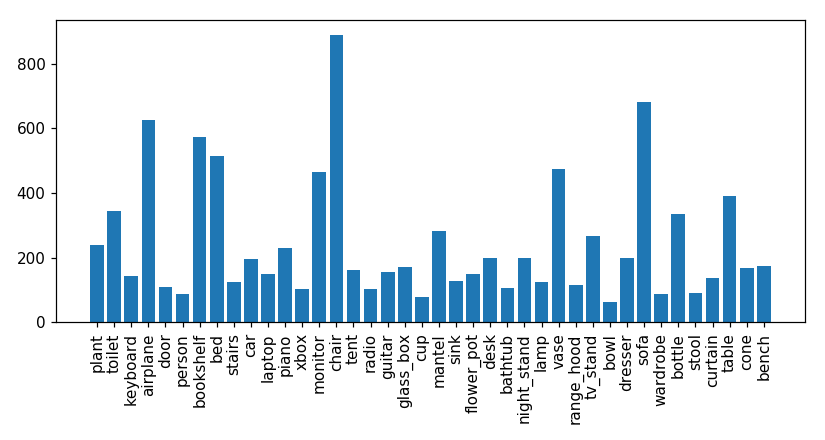
\includegraphics[width=\textwidth]{Figures/shape_retrieval/modelnet_classes.png}
    \caption{ModelNet40 data set: distribution of samples per class.}
    \label{fig:modelnet_classes}
\end{figure}

\subsection{Implementation details}
To demonstrate the impact that the triplet based training has on the performance of CNN descriptors
we use a deep network architecture shown in a Table~\ref{tab:net-architecture}. This network was implemented in PySparseConvNet, which is our modification of the SparseConvNet library \cite{graham2014spatially}. Besides new loss functions PySparseConvNet can be accessed from Python for a more interactive usage.

When forming a triplet for training we choose uniformly randomly a positive pair of objects from one class
and select a negative sample uniformly randomly from one of other classes.

For the optimization we use the SGD \cite{bottou-tricks-2012}, and the training is done
\begin{itemize}
\item in batches of size from $45$ to $90$ depending on a GPU video memory,
\item with a learning rate of $0.002$,
\item and a momentum equal to $0.99$.
\end{itemize}
Training can take up to a week on a server with advanced GPU, such as NVIDIA Titan X or GTX980ti.

\begin{figure}
\centering
\begin{tabular}{ccccc}
  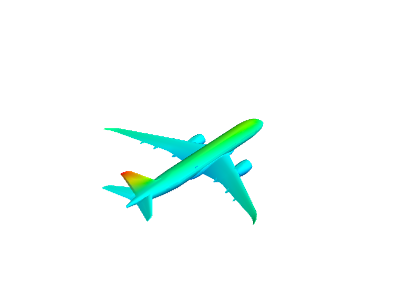
\includegraphics[width=0.19\columnwidth]{Figures/shape_retrieval/pic_airplane_solid.png} &
  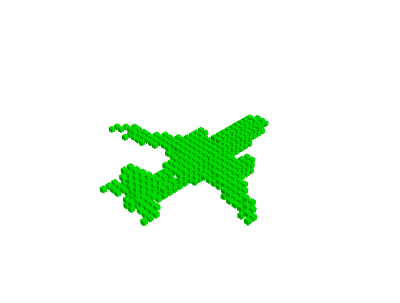
\includegraphics[width=0.19\columnwidth]{Figures/shape_retrieval/pic_airplane_30_solid.png} &
  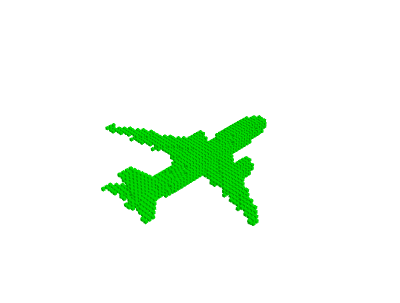
\includegraphics[width=0.19\columnwidth]{Figures/shape_retrieval/pic_airplane_50_solid.png} &
  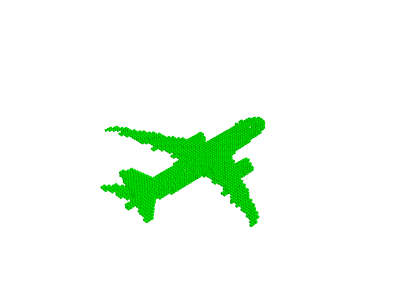
\includegraphics[width=0.19\columnwidth]{Figures/shape_retrieval/pic_airplane_70_solid.png} &
  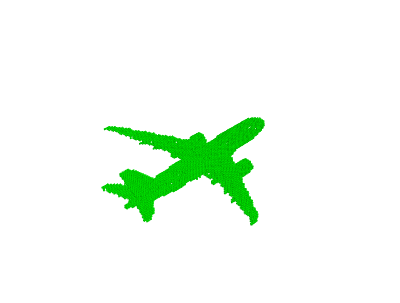
\includegraphics[width=0.19\columnwidth]{Figures/shape_retrieval/pic_airplane_100_solid.png} \\
% (a) first & (b) second \\
 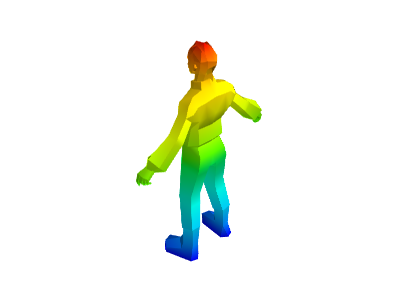
\includegraphics[width=0.19\columnwidth]{Figures/shape_retrieval/pic_person_solid.png} &
 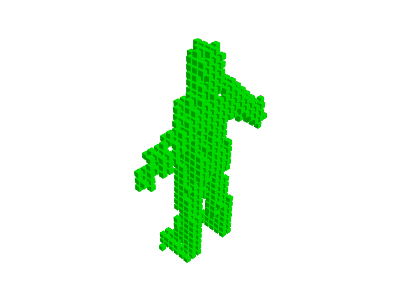
\includegraphics[width=0.19\columnwidth]{Figures/shape_retrieval/pic_person_30_solid.png} &
 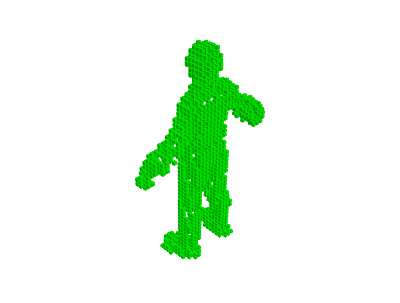
\includegraphics[width=0.19\columnwidth]{Figures/shape_retrieval/pic_person_50_solid.png} &
 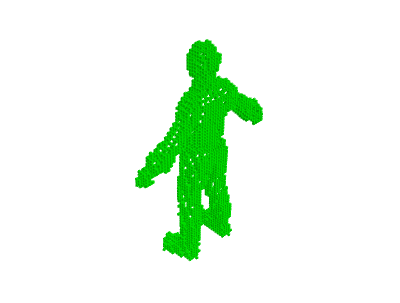
\includegraphics[width=0.19\columnwidth]{Figures/shape_retrieval/pic_person_70_solid.png} &
 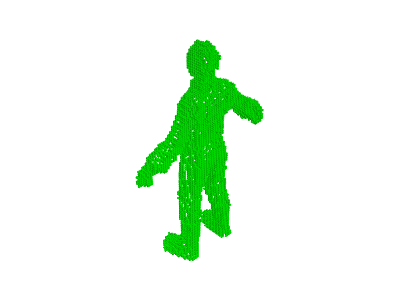
\includegraphics[width=0.19\columnwidth]{Figures/shape_retrieval/pic_person_100_solid.png} \\

 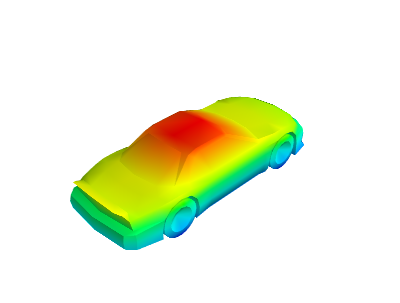
\includegraphics[width=0.19\columnwidth]{Figures/shape_retrieval/pic_car_solid.png} &
 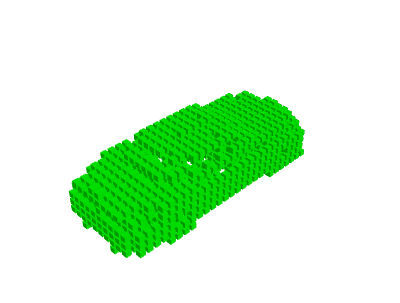
\includegraphics[width=0.19\columnwidth]{Figures/shape_retrieval/pic_car_30_solid.png} &
 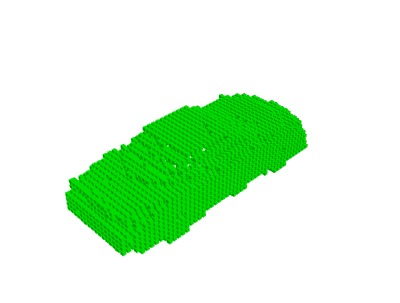
\includegraphics[width=0.19\columnwidth]{Figures/shape_retrieval/pic_car_50_solid.png} &
 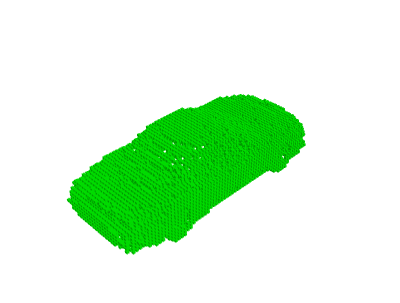
\includegraphics[width=0.19\columnwidth]{Figures/shape_retrieval/pic_car_70_solid.png} &
 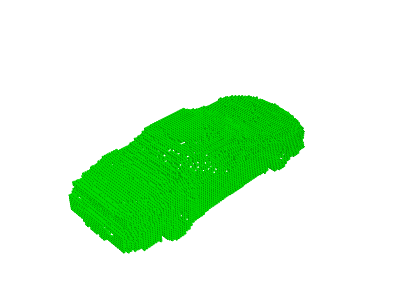
\includegraphics[width=0.19\columnwidth]{Figures/shape_retrieval/pic_car_100_solid.png} \\
\end{tabular}
\caption{Examples of some objects voxelizations at different resolutions $30$, $50$, $70$, $100$ (from left to right), left-most objects are depicted using original meshes}
\label{fig:voxels-examples}
\end{figure}


We train Sparse 3D Convolutional Neural Network (S3DCNN) on the 3D shape classification dataset by splitting it into  training and validation subsets, adding augmentation of data to achieve rotational and translational invariance. After training a model on a dataset of pairs, we use it to embed voxel representations of 3D meshes into $192$-dimensional space. The retrieval consist of ranking search objects by a cosine distance of vectors from a query vector.

The most popular metrics for evaluating retrieval performance are
\begin{itemize}
\item Precision-Recall Curve shows a trade-off between these two measures and how quickly the precision drops with the recall increase,
\item Mean average precision (mAP). Given a query, its average precision is the average of all precision values computed on all relevant objects in the retrieved list. Given several queries, the mean average precision (mAP) is the mean of average precisions for these queries. 
\end{itemize}
We evaluated mAP for different voxel rendering sizes of 3D shapes both at train and test times, see also Figure~\ref{fig:voxels-examples}.

To check if our model is comparable with other architectures, we consider a classification task. So, we trained our model for the classification task using the ModelNet40 train subset with 
\begin{itemize}
\item SoftMax last layer for $200$ epochs,
\item with exponentially discounting learning rate,
\item and performed retrieval evaluation on the test subset,
\item taking $20$ images from every class, and ranking them w.r.t their $L2$-norm by activations taken from the $17$-th layer.
\end{itemize}

Results of these experiments are provided in Table~\ref{tab:classification}. We can see that in case of classification task setup our model is comparable in terms of the classification accuracy, but mAP values are worse. But in case of metric learning performace of S3DCNN on mAP metric is much better.
Superior performance of retrieval task with MVCNN is not a surprising result, since MVCNN uses neural nets, pre-trained on ImageNet. On the other hand our model only requires 3D Shape dataset to learn.

In Figure~\ref{fig:map_for_rs} we provide the dependence of mAP on the input spatial resolution. We can see that the retrieval performance improves with increase in the input spatial resolution up to around $45-50$, after that it drops slightly and goes to plateau. It can be attributed to the insufficient amount of layers for the same scale of features, that can be separated in higher layers. Light blue color shows range of mAP on validation for top $30$ trained architectures.


\begin{figure}[!tbp]
\vspace{-20pt}
\centering
\begin{minipage}[b]{0.45\textwidth}
  \centering
  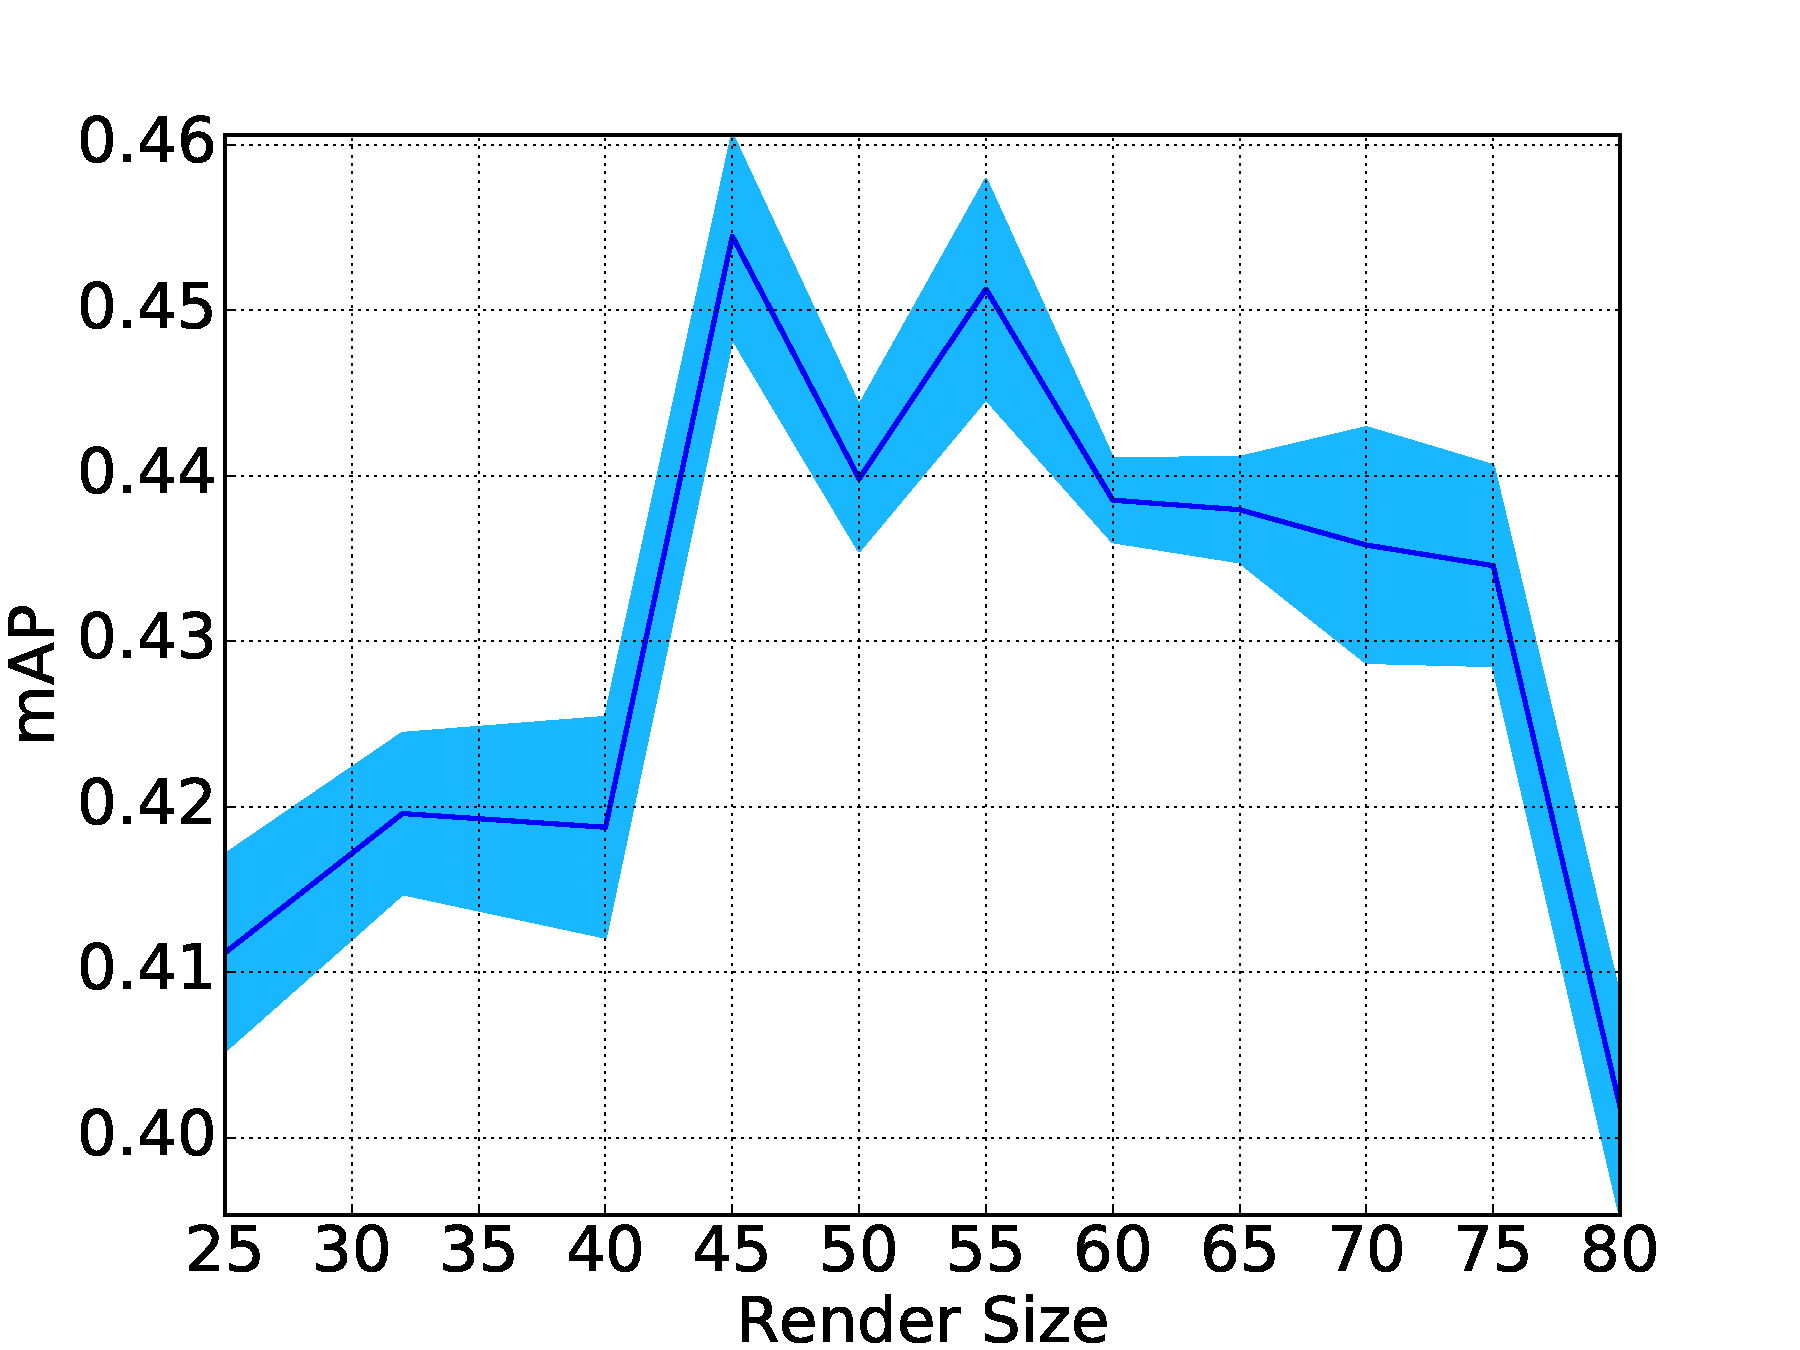
\includegraphics[width=\columnwidth]{Figures/shape_retrieval/new_map_to_rs.pdf}
  \caption{Dependence of the retrieval performance on the input spatial resolution}
  \label{fig:map_for_rs}
\end{minipage}
\begin{minipage}[b]{0.45\textwidth}
  \centering
  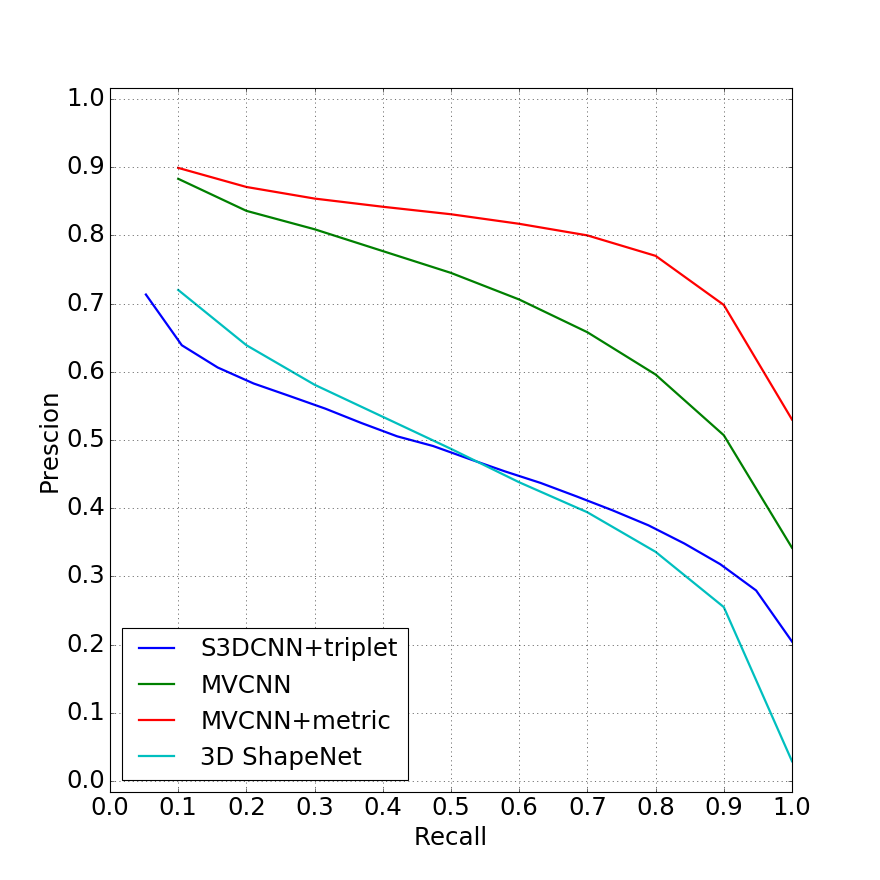
\includegraphics[width=\columnwidth]{Figures/shape_retrieval/pr_curves_comp}
  \caption{Precision-Recall curve for our method}
  \label{fig:pr_curve}
\end{minipage}
\end{figure}


We would like to note that in Figure~\ref{fig:map_for_rs} mAP values provided for different validation epochs and variability of best model can be explained by difference in total learning time.

% \begin{itemize}
% \item In Table~\ref{tab:classification} for the retrieval we used features from the last but one layer of the network,
% \item In Figure~\ref{fig:map_for_rs} we used learning with the triplet loss, for which we still have to better adjust the architecture and learning rate schedule.
% \end{itemize}


\section{Results}
\label{sec:5}

\begin{figure}
  \centering
    \includegraphics[width=\textwidth]{Figures/shape_retrieval/cnn_embed_2k.jpg}
    \caption{t-SNE plot of ModelNet40 validation set}
    \label{fig:modelnet_tsne}
\end{figure}

We found that the retrieval performance improves with increase in the input spatial resolution. However, such an effect is difficult to check experimentally and to use in practice, as e.g. for usual 3D dense CNNs the computational time is prohibitively large. In our case, data sparsity helps us to process data in reasonable time even with input resolution up to $100^3$ voxels, therefore we can benefit from the increase of the input spatial resolution when performing retrieval.
In Figure~\ref{fig:pr_curve} we can see that our method is comparable to \cite{wu20153d} in low recall, and better at higher recall values, that indicates better scalability of our method.
In Table~\ref{tab:classification} for the retrieval we used features from the one before last layer of the network of size 192, which in  comparison to 4000 in 3DShapeNet model \cite{wu20153d} is 20 times smaller but achieves almost the same retrieval metrics.


We evaluated our network architecture described in Table~\ref{tab:net-architecture} on popular state-of-the-art frameworks for Deep Learning, such as Tensorflow~\cite{tensorflow2015-whitepaper} on GPU and \cite{2016arXiv160502688short} on CPU.
Using Keras \cite{chollet2015keras} 2.0.2 with Tensorflow~\cite{tensorflow2015-whitepaper} 1.2.1 backend on Nvidia Titan X GPU with 12Gb of GPU memory, we were able to exhaust all of it with batch size equal to 12, and performed forward passes on average 0.0301 seconds/sample, which is comparable to processing speed of our implementation with render size of about 60-70.
Other setup was an implementation of our network architecture on Keras with Theano backend using Intel i7-5820K 6-core CPU processor, took 1.53 seconds/sample, which is significantly slower.
% We provide training code for all experiments in our repository\footnote{\url{https://github.com/gangiman/PySparseConvNet}}.


\begin{table}[t]
  \caption{Evaluation on Modelnet40}
  \label{tab:classification}
  \centering
  \begin{tabular}{llll}
    \toprule
    method & Classification & Retrieval AUC & Retrieval mAP \\
    \midrule
    3DShapeNet \cite{wu20153d} & 77.32\% & 49.94\% & 49.23\% \\
    MVCNN \cite{su15mvcnn} & 90.10\% & --- & 80.20\% \\
    VoxNet \cite{maturana2015voxnet} & 83.00\% & --- & --- \\
    VRN \cite{brock2016generative} & 91.33\% & --- & --- \\
    \textbf{S3DCNN (proposed)} & \textbf{90.30}\% & \textbf{36.05}\% & \textbf{33.67}\% \\
    \textbf{S3DCNN + triplet (proposed)} & --- & \textbf{48.81}\% & \textbf{46.71}\% \\
    \bottomrule
  \end{tabular}
\end{table}

\subsubsection*{Acknowledgments}
We are very grateful to Dmitry Yarotsky for his contribution to this research project. Big Thanks to Benjamin Graham for some useful comments and ideas. Thanks to Rasim Akhunzyanov for his help in debugging the PySparseConvNet code.

The research was partially supported by the Russian Science Foundation grant (project 14-50-00150).

% \clearpage
% \bibliographystyle{abbrv}
% \bibliography{bibliography}

% \end{document}

\newpage 
% \documentclass[10pt,twocolumn,letterpaper]{article}

% \usepackage[dvipsnames]{xcolor}
% \usepackage{cvpr}
% \usepackage{times}
% \usepackage{epsfig}
% \usepackage{graphicx}[draft]
% \usepackage{amsmath}
% \usepackage{amssymb}
% \usepackage{array,colortbl,multirow,multicol,booktabs,ctable}
% \usepackage{bm}
% \usepackage{subfig}
% % The LaTeX graphics/graphicx package uses the first 
% % dot to find the extension. Package grffile changes 
% % the algorithm to check for known extensions (option multidot, enabled by default):
% \usepackage{grffile} 
% \usepackage{dblfloatfix}

% % Include other packages here, before hyperref.

% % If you comment hyperref and then uncomment it, you should delete
% % egpaper.aux before re-running latex.  (Or just hit 'q' on the first latex
% % run, let it finish, and you should be clear).
% \usepackage[pagebackref=true,breaklinks=true,letterpaper=true,colorlinks,bookmarks=false]{hyperref}

% % \cvprfinalcopy % *** Uncomment this line for the final submission

% \def\cvprPaperID{4968} % *** Enter the CVPR Paper ID here
% \def\httilde{\mbox{\tt\raisebox{-.5ex}{\symbol{126}}}}

% % Pages are numbered in submission mode, and unnumbered in camera-ready
% \ifcvprfinal\pagestyle{empty}\fi

% \renewcommand{\floatpagefraction}{.9}
% \renewcommand{\textfraction}{.1}

% \renewcommand{\baselinestretch}{0.955}
% \renewcommand{\paragraph}[1]{\noindent{\bf #1}}

% \begin{document}

% %%%%%%%%% TITLE
% \title{Perceptually-Based Single-Image Depth Super-Resolution}
\chapter{Perceptually-Based Single-Image Depth Super-Resolution}

% \author{First Author\\
% Institution1\\
% Institution1 address\\
% {\tt\small firstauthor
% @i1.org}
% % For a paper whose authors are all at the same institution,
% % omit the following lines up until the closing ``}''.
% % Additional authors and addresses can be added with ``\and'',
% % just like the second author.
% % To save space, use either the email address or home page, not both
% \and
% Second Author\\
% Institution2\\
% First line of institution2 address\\
% {\tt\small secondauthor@i2.org}
% }

% \maketitle
% %\thispagestyle{empty}
\input Chapters/depth_superresolution/00-pre.tex

% %%%%%%%%% ABSTRACT
% \begin{abstract}
% RGBD images, combining high-resolution color and lower-resolution depth from various types of depth sensors, are increasingly common. One can significantly improve the resolution of depth images by taking advantage of color information; deep learning methods make combining color and depth information particularly easy. 
% However, fusing these two sources of data may lead to a variety of artifacts.  If depth maps are used to reconstruct 3D shapes, e.g., for virtual reality applications, the visual quality of upsampled images is particularly important.  To achieve high-quality results, visual metric need to be taken into account. 
% The main idea of our approach is to measure the quality of depth map upsampling using renderings of
% resulting 3D surfaces.  We demonstrate that a simple visual appearance-based loss, when used with either a trained CNN or simply a deep prior, yields significantly improved 3D shapes, as measured by a number of existing perceptual metrics. We compare this approach with a number of existing optimization and learning-based techniques.
% \end{abstract}

%%%%%%%%% BODY TEXT
\input Chapters/depth_superresolution/01-motivation.tex
% \input Chapters/depth_superresolution/02-related.tex
\input Chapters/depth_superresolution/03-visual.tex
\input Chapters/depth_superresolution/04-methods.tex
\input Chapters/depth_superresolution/05-exper.tex
\input Chapters/depth_superresolution/06-concl.tex





% Please follow the steps outlined below when submitting your manuscript to
% the IEEE Computer Society Press.  This style guide now has several
% important modifications (for example, you are no longer warned against the
% use of sticky tape to attach your artwork to the paper), so all authors
% should read this new version.

% %-------------------------------------------------------------------------
% \subsection{Language}

% All manuscripts must be in English.

% \subsection{Dual submission}

% Please refer to the author guidelines on the CVPR 2018 web page for a
% discussion of the policy on dual submissions.

% \subsection{Paper length}
% Papers, excluding the references section,
% must be no longer than eight pages in length. The references section
% will not be included in the page count, and there is no limit on the
% length of the references section. For example, a paper of eight pages
% with two pages of references would have a total length of 10 pages.
% {\bf There will be no extra page charges for CVPR 2018.}

% Overlength papers will simply not be reviewed.  This includes papers
% where the margins and formatting are deemed to have been significantly
% altered from those laid down by this style guide.  Note that this
% \LaTeX\ guide already sets figure captions and references in a smaller font.
% The reason such papers will not be reviewed is that there is no provision for
% supervised revisions of manuscripts.  The reviewing process cannot determine
% the suitability of the paper for presentation in eight pages if it is
% reviewed in eleven.  

% %-------------------------------------------------------------------------
% \subsection{The ruler}
% The \LaTeX\ style defines a printed ruler which should be present in the
% version submitted for review.  The ruler is provided in order that
% reviewers may comment on particular lines in the paper without
% circumlocution.  If you are preparing a document using a non-\LaTeX\
% document preparation system, please arrange for an equivalent ruler to
% appear on the final output pages.  The presence or absence of the ruler
% should not change the appearance of any other content on the page.  The
% camera ready copy should not contain a ruler. (\LaTeX\ users may uncomment
% the \verb'\cvprfinalcopy' command in the document preamble.)  Reviewers:
% note that the ruler measurements do not align well with lines in the paper
% --- this turns out to be very difficult to do well when the paper contains
% many figures and equations, and, when done, looks ugly.  Just use fractional
% references (e.g.\ this line is $095.5$), although in most cases one would
% expect that the approximate location will be adequate.

% \subsection{Mathematics}

% Please number all of your sections and displayed equations.  It is
% important for readers to be able to refer to any particular equation.  Just
% because you didn't refer to it in the text doesn't mean some future reader
% might not need to refer to it.  It is cumbersome to have to use
% circumlocutions like ``the equation second from the top of page 3 column
% 1''.  (Note that the ruler will not be present in the final copy, so is not
% an alternative to equation numbers).  All authors will benefit from reading
% Mermin's description of how to write mathematics:
% \url{http://www.pamitc.org/documents/mermin.pdf}.


% \subsection{Blind review}

% Many authors misunderstand the concept of anonymizing for blind
% review.  Blind review does not mean that one must remove
% citations to one's own work---in fact it is often impossible to
% review a paper unless the previous citations are known and
% available.

% Blind review means that you do not use the words ``my'' or ``our''
% when citing previous work.  That is all.  (But see below for
% techreports.)

% Saying ``this builds on the work of Lucy Smith [1]'' does not say
% that you are Lucy Smith; it says that you are building on her
% work.  If you are Smith and Jones, do not say ``as we show in
% [7]'', say ``as Smith and Jones show in [7]'' and at the end of the
% paper, include reference 7 as you would any other cited work.

% An example of a bad paper just asking to be rejected:
% \begin{quote}
% \begin{center}
%     An analysis of the frobnicatable foo filter.
% \end{center}

%   In this paper we present a performance analysis of our
%   previous paper [1], and show it to be inferior to all
%   previously known methods.  Why the previous paper was
%   accepted without this analysis is beyond me.

%   [1] Removed for blind review
% \end{quote}


% An example of an acceptable paper:

% \begin{quote}
% \begin{center}
%      An analysis of the frobnicatable foo filter.
% \end{center}

%   In this paper we present a performance analysis of the
%   paper of Smith \etal [1], and show it to be inferior to
%   all previously known methods.  Why the previous paper
%   was accepted without this analysis is beyond me.

%   [1] Smith, L and Jones, C. ``The frobnicatable foo
%   filter, a fundamental contribution to human knowledge''.
%   Nature 381(12), 1-213.
% \end{quote}

% If you are making a submission to another conference at the same time,
% which covers similar or overlapping material, you may need to refer to that
% submission in order to explain the differences, just as you would if you
% had previously published related work.  In such cases, include the
% anonymized parallel submission~\cite{Authors14} as additional material and
% cite it as
% \begin{quote}
% [1] Authors. ``The frobnicatable foo filter'', F\&G 2014 Submission ID 324,
% Supplied as additional material {\tt fg324.pdf}.
% \end{quote}

% Finally, you may feel you need to tell the reader that more details can be
% found elsewhere, and refer them to a technical report.  For conference
% submissions, the paper must stand on its own, and not {\em require} the
% reviewer to go to a techreport for further details.  Thus, you may say in
% the body of the paper ``further details may be found
% in~\cite{Authors14b}''.  Then submit the techreport as additional material.
% Again, you may not assume the reviewers will read this material.

% Sometimes your paper is about a problem which you tested using a tool which
% is widely known to be restricted to a single institution.  For example,
% let's say it's 1969, you have solved a key problem on the Apollo lander,
% and you believe that the CVPR70 audience would like to hear about your
% solution.  The work is a development of your celebrated 1968 paper entitled
% ``Zero-g frobnication: How being the only people in the world with access to
% the Apollo lander source code makes us a wow at parties'', by Zeus \etal.

% You can handle this paper like any other.  Don't write ``We show how to
% improve our previous work [Anonymous, 1968].  This time we tested the
% algorithm on a lunar lander [name of lander removed for blind review]''.
% That would be silly, and would immediately identify the authors. Instead
% write the following:
% \begin{quotation}
% \noindent
%   We describe a system for zero-g frobnication.  This
%   system is new because it handles the following cases:
%   A, B.  Previous systems [Zeus et al. 1968] didn't
%   handle case B properly.  Ours handles it by including
%   a foo term in the bar integral.

%   ...

%   The proposed system was integrated with the Apollo
%   lunar lander, and went all the way to the moon, don't
%   you know.  It displayed the following behaviours
%   which show how well we solved cases A and B: ...
% \end{quotation}
% As you can see, the above text follows standard scientific convention,
% reads better than the first version, and does not explicitly name you as
% the authors.  A reviewer might think it likely that the new paper was
% written by Zeus \etal, but cannot make any decision based on that guess.
% He or she would have to be sure that no other authors could have been
% contracted to solve problem B.
% \medskip

% \noindent
% FAQ\medskip\\
% {\bf Q:} Are acknowledgements OK?\\
% {\bf A:} No.  Leave them for the final copy.\medskip\\
% {\bf Q:} How do I cite my results reported in open challenges?
% {\bf A:} To conform with the double blind review policy, you can report results of other challenge participants together with your results in your paper. For your results, however, you should not identify yourself and should not mention your participation in the challenge. Instead present your results referring to the method proposed in your paper and draw conclusions based on the experimental comparison to other results.\medskip\\

% \begin{figure}[t]
% \begin{center}
% \fbox{\rule{0pt}{2in} \rule{0.9\linewidth}{0pt}}
%   %\includegraphics[width=0.8\linewidth]{egfigure.eps}
% \end{center}
%   \caption{Example of caption.  It is set in Roman so that mathematics
%   (always set in Roman: $B \sin A = A \sin B$) may be included without an
%   ugly clash.}
% \label{fig:long}
% \label{fig:onecol}
% \end{figure}

% \subsection{Miscellaneous}

% \noindent
% Compare the following:\\
% \begin{tabular}{ll}
%  \verb'$conf_a$' &  $conf_a$ \\
%  \verb'$\mathit{conf}_a$' & $\mathit{conf}_a$
% \end{tabular}\\
% See The \TeX book, p165.

% The space after \eg, meaning ``for example'', should not be a
% sentence-ending space. So \eg is correct, {\em e.g.} is not.  The provided
% \verb'\eg' macro takes care of this.

% When citing a multi-author paper, you may save space by using ``et alia'',
% shortened to ``\etal'' (not ``{\em et.\ al.}'' as ``{\em et}'' is a complete word.)
% However, use it only when there are three or more authors.  Thus, the
% following is correct: ``
%   Frobnication has been trendy lately.
%   It was introduced by Alpher~\cite{Alpher02}, and subsequently developed by
%   Alpher and Fotheringham-Smythe~\cite{Alpher03}, and Alpher \etal~\cite{Alpher04}.''

% This is incorrect: ``... subsequently developed by Alpher \etal~\cite{Alpher03} ...''
% because reference~\cite{Alpher03} has just two authors.  If you use the
% \verb'\etal' macro provided, then you need not worry about double periods
% when used at the end of a sentence as in Alpher \etal.

% For this citation style, keep multiple citations in numerical (not
% chronological) order, so prefer \cite{Alpher03,Alpher02,Authors14} to
% \cite{Alpher02,Alpher03,Authors14}.


% \begin{figure*}
% \begin{center}
% \fbox{\rule{0pt}{2in} \rule{.9\linewidth}{0pt}}
% \end{center}
%   \caption{Example of a short caption, which should be centered.}
% \label{fig:short}
% \end{figure*}

% %------------------------------------------------------------------------
% \section{Formatting your paper}

% All text must be in a two-column format. The total allowable width of the
% text area is $6\frac78$ inches (17.5 cm) wide by $8\frac78$ inches (22.54
% cm) high. Columns are to be $3\frac14$ inches (8.25 cm) wide, with a
% $\frac{5}{16}$ inch (0.8 cm) space between them. The main title (on the
% first page) should begin 1.0 inch (2.54 cm) from the top edge of the
% page. The second and following pages should begin 1.0 inch (2.54 cm) from
% the top edge. On all pages, the bottom margin should be 1-1/8 inches (2.86
% cm) from the bottom edge of the page for $8.5 \times 11$-inch paper; for A4
% paper, approximately 1-5/8 inches (4.13 cm) from the bottom edge of the
% page.

% %-------------------------------------------------------------------------
% \subsection{Margins and page numbering}

% All printed material, including text, illustrations, and charts, must be kept
% within a print area 6-7/8 inches (17.5 cm) wide by 8-7/8 inches (22.54 cm)
% high.



% %-------------------------------------------------------------------------
% \subsection{Type-style and fonts}

% Wherever Times is specified, Times Roman may also be used. If neither is
% available on your word processor, please use the font closest in
% appearance to Times to which you have access.

% MAIN TITLE. Center the title 1-3/8 inches (3.49 cm) from the top edge of
% the first page. The title should be in Times 14-point, boldface type.
% Capitalize the first letter of nouns, pronouns, verbs, adjectives, and
% adverbs; do not capitalize articles, coordinate conjunctions, or
% prepositions (unless the title begins with such a word). Leave two blank
% lines after the title.

% AUTHOR NAME(s) and AFFILIATION(s) are to be centered beneath the title
% and printed in Times 12-point, non-boldface type. This information is to
% be followed by two blank lines.

% The ABSTRACT and MAIN TEXT are to be in a two-column format.

% MAIN TEXT. Type main text in 10-point Times, single-spaced. Do NOT use
% double-spacing. All paragraphs should be indented 1 pica (approx. 1/6
% inch or 0.422 cm). Make sure your text is fully justified---that is,
% flush left and flush right. Please do not place any additional blank
% lines between paragraphs.

% Figure and table captions should be 9-point Roman type as in
% Figures~\ref{fig:onecol} and~\ref{fig:short}.  Short captions should be centred.

% \noindent Callouts should be 9-point Helvetica, non-boldface type.
% Initially capitalize only the first word of section titles and first-,
% second-, and third-order headings.

% FIRST-ORDER HEADINGS. (For example, {\large \bf 1. Introduction})
% should be Times 12-point boldface, initially capitalized, flush left,
% with one blank line before, and one blank line after.

% SECOND-ORDER HEADINGS. (For example, { \bf 1.1. Database elements})
% should be Times 11-point boldface, initially capitalized, flush left,
% with one blank line before, and one after. If you require a third-order
% heading (we discourage it), use 10-point Times, boldface, initially
% capitalized, flush left, preceded by one blank line, followed by a period
% and your text on the same line.

% %-------------------------------------------------------------------------
% \subsection{Footnotes}

% Please use footnotes\footnote {This is what a footnote looks like.  It
% often distracts the reader from the main flow of the argument.} sparingly.
% Indeed, try to avoid footnotes altogether and include necessary peripheral
% observations in
% the text (within parentheses, if you prefer, as in this sentence).  If you
% wish to use a footnote, place it at the bottom of the column on the page on
% which it is referenced. Use Times 8-point type, single-spaced.


% %-------------------------------------------------------------------------
% \subsection{References}

% List and number all bibliographical references in 9-point Times,
% single-spaced, at the end of your paper. When referenced in the text,
% enclose the citation number in square brackets, for
% example~\cite{Authors14}.  Where appropriate, include the name(s) of
% editors of referenced books.

% \begin{table}
% \begin{center}
% \begin{tabular}{|l|c|}
% \hline
% Method & Frobnability \\
% \hline\hline
% Theirs & Frumpy \\
% Yours & Frobbly \\
% Ours & Makes one's heart Frob\\
% \hline
% \end{tabular}
% \end{center}
% \caption{Results.   Ours is better.}
% \end{table}

% %-------------------------------------------------------------------------
% \subsection{Illustrations, graphs, and photographs}

% All graphics should be centered.  Please ensure that any point you wish to
% make is resolvable in a printed copy of the paper.  Resize fonts in figures
% to match the font in the body text, and choose line widths which render
% effectively in print.  Many readers (and reviewers), even of an electronic
% copy, will choose to print your paper in order to read it.  You cannot
% insist that they do otherwise, and therefore must not assume that they can
% zoom in to see tiny details on a graphic.

% When placing figures in \LaTeX, it's almost always best to use
% \verb+\includegraphics+, and to specify the  figure width as a multiple of
% the line width as in the example below
% {\small\begin{verbatim}
%   \usepackage[dvips]{graphicx} ...
%   \includegraphics[width=0.8\linewidth]
%                   {myfile.eps}
% \end{verbatim}
% }


% %-------------------------------------------------------------------------
% \subsection{Color}

% Please refer to the author guidelines on the CVPR 2018 web page for a discussion
% of the use of color in your document.

% %------------------------------------------------------------------------
% \section{Final copy}

% You must include your signed IEEE copyright release form when you submit
% your finished paper. We MUST have this form before your paper can be
% published in the proceedings.

% Please direct any questions to the production editor in charge of these
% proceedings at the IEEE Computer Society Press: Phone (714) 821-8380, or
% Fax (714) 761-1784.


% \clearpage
% \newpage

% {\small
% \bibliographystyle{ieee}
% \bibliography{egbib}
% }

% \clearpage
% \newpage
% \input 07-supp.tex

% \end{document}

\newpage 
% \documentclass[10pt,twocolumn,letterpaper]{article}

% \usepackage{wacv}
% \usepackage{times}
% \usepackage{epsfig}
% \usepackage{graphicx}
% \usepackage{amsmath}
% \usepackage{amssymb}
% \usepackage{placeins}
% % \usepackage{authblk}

% % Include other packages here, before hyperref.



% %%%%%%%%%%%%%%%%%%%%%%%%%%%%%%%%%%%%%%%%%%%%%%%%%%%%%%%%%%%%%%%%%%%%%%%%%%%%%%%%
% %
% %%% IMPORTANT - These next three lines are crucial.
% %               (1) PLEASE enter your paper ID (given by CMT) replacing the
% %                   '****' right below here with the ID from CMT.
% %               (2) Leave the \wacvfinacopy commented out for the submission
% %                   version, but UNCOMMENT it for your CAMERA-READY upload.
% %               (3) For the camera-ready version, you may be asked to set a
% %                   starting page number.  If so, replace the '9876' below with
% %                   the starting page number assigned by the publication chair.
 
% %(1)
% \def\wacvPaperID{410} % Enter the WACV Paper ID here

% %(2)
% \wacvfinalcopy % *** Uncomment this line for the final submission

% %(3)
% \ifwacvfinal
% \def\assignedStartPage{1} % *** Enter the assigned starting page number (instead of 9876)
% \fi

% %%%%%%%%%%%%%%%%%%%%%%%%%%%%%%%%%%%%%%%%%%%%%%%%%%%%%%%%%%%%%%%%%%%%%%%%%%%%%%%%

% % If you comment hyperref and then uncomment it, you should delete
% % egpaper.aux before re-running latex.  (Or just hit 'q' on the first latex
% % run, let it finish, and you should be clear).
% % \usepackage{hyperref}
% \ifwacvfinal
% \usepackage{hyperref}
% \hypersetup{breaklinks=true,bookmarks=false}
% \else
% \usepackage{hyperref}
% \hypersetup{pagebackref=true,breaklinks=true,colorlinks,bookmarks=false}
% \fi

% % Pages are numbered in submission mode, and unnumbered in camera-ready
% \ifwacvfinal
% \setcounter{page}{\assignedStartPage}
% \else
% \pagestyle{empty}
% \fi

% \def\httilde{\mbox{\tt\raisebox{-.5ex}{\symbol{126}}}}

% \begin{document}

%%%%%%%%% TITLE
% \title{Making DensePose fast and light}
\chapter{Making DensePose fast and light}

% \author{
%     Ruslan Rakhimov\textsuperscript{1}\thanks{Equal contribution}\space, 
%     Emil Bogomolov\textsuperscript{1}$^*$, 
%     Alexandr Notchenko\textsuperscript{1},\\
%     Fung Mao\textsuperscript{2}, 
%     Alexey Artemov\textsuperscript{1}, 
%     Denis Zorin\textsuperscript{1,3}, 
%     Evgeny Burnaev\textsuperscript{1}\\
%     \textsuperscript{1}{\small Skolkovo Institute of Science and Technology}\\
%     \textsuperscript{2}{\small Huawei Moscow Research Center (Russia)}\\
%     \textsuperscript{3}{\small New York University}\\
%     {\tt\small\{ruslan.rakhimov, e.bogomolov, alexandr.notchenko\}@skoltech.ru,}\\
%     {\tt\small fung.mao@huawei.com, a.artemov@skoltech.ru, dzorin@cs.nyu.edu, e.burnaev@skoltech.ru}\\
% }

% \author{%
%     Ruslan Rakhimov\textsuperscript{1}\thanks{Equal contribution} \\
%     {\tt\small ruslan.rakhimov@skoltech.ru}
%     \and
%     Emil Bogomolov\textsuperscript{1}$^*$ \\
%     {\tt\small e.bogomolov@skoltech.ru}
%     \and
%     Alexandr Notchenko\textsuperscript{1} \\
%     {\tt\small alexandr.notchenko@skolkovotech.ru}
%     \and
%     Fung Mao\textsuperscript{2} \\
%     {\tt\small fung.mao@huawei.com}
%     \and
%     Alexey Artemov\textsuperscript{1} \\
%     {\tt\small a.artemov@skoltech.ru}
%     \and\and\and
%     Denis Zorin\textsuperscript{1,3} \\
%     {\tt\small dzorin@cs.nyu.edu}
%     \and\and\and
%     Evgeny Burnaev\textsuperscript{1} \\
%     {\tt\small e.burnaev@skoltech.ru}
%     \and\and\and
%     \textsuperscript{1}{\small Skolkovo Institute of Science and Technology}\\
%     \textsuperscript{2}{\small Huawei Moscow Research Center (Russia)}\\
%     \textsuperscript{3}{\small New York University}
% }

% \author[1]{Ruslan Rakhimov\thanks{Equal contribution}}
% \author[1]{Emil Bogomolov$^*$}
% \author[1]{Alexandr Notchenko}
% \author[2]{Fung Mao}
% \author[1]{Alexey Artemov}
% \author[1,3]{Denis Zorin}
% \author[1]{Evgeny Burnaev}

% \affil[1]{Skolkovo Institute of Science and Technology,\{ruslan.rakhimov,e.bogomolov,alexandr.notchenko,a.artemov,e.burnaev\}}
% \affil[2]{Huawei Moscow Research Center (Russia)}
% \affil[3]{New York University}


% \affil[1]{University of Southern California, Los Angeles, CA \authorcr Email: {\tt \{uid1, uid2\}@usc.edu}\vspace{1.5ex}}
% \affil[2]{NASA Jet Propulsion Laboratory, Pasadena, CA \authorcr Email: {\tt uid3@jpl.nasa.gov} \vspace{-2ex}} 

% \author[1]{Ruslan Rakhimov\thanks{Equal contribution}\\ ruslan.rakhimov@skoltech.ru}
% \author[2]{Emil Bogomolov$^*$\\{\tt\small e.bogomolov@skoltech.ru}}
% \affil[1]{Department of Mathematics, University X}
% \affil[2]{Department of Biology, University Y}

% \maketitle
%\thispagestyle{empty}

%%%%%%%%% ABSTRACT

% \begin{abstract}
DensePose estimation task is a significant step forward for enhancing user experience computer vision applications ranging from augmented reality to cloth fitting. Existing neural network models capable of solving this task are heavily parameterized and a long way from being transferred to an embedded or mobile device. To enable Dense Pose inference on the end device with current models, one needs to support an expensive server-side infrastructure and have a stable internet connection. To make things worse, mobile and embedded devices do not always have a powerful GPU inside.
In this work, we target the problem of redesigning the DensePose R-CNN model's architecture so that the final network retains most of its accuracy but becomes more light-weight and fast. To achieve that, we tested and incorporated many deep learning innovations from recent years, specifically performing an ablation study on 23 efficient backbone architectures, multiple two-stage detection pipeline modifications, and custom model quantization methods. 
As a result, we achieved $17\times$ model size reduction and $2\times$ latency improvement compared to the baseline model.\ifwacvfinal\footnote{Code is available at \url{https://github.com/zetyquickly/DensePoseFnL}}\fi
\end{abstract}
% \section{Introduction}

This work is dedicated to developing an architecture for solving DensePose \cite{densepose} estimation task with a particular requirement: the model should be light-weight and run in real-time on a mobile device.

The task of understanding humans in an image may involve different formulations of the problem: 2d landmarks localization, human part segmentation, 3d reconstruction, dense image-to-surface correspondences (DensePose). In this work, we target the multi-person formulation of DensePose task: given a single RGB image solve the regression task: for each pixel, find its surface points (UV coordinates) on a deformable surface model (the Skinned Multi-Person Linear (SMPL) model \cite{smpl}).

Finding surface correspondence is a step forward to a general 3d human representation. Possible applications lie in such fields, like augmented reality, virtual fitting rooms. Densepose output may serve as input to another model. For instance, it was used as an input in video-to-video translation tasks \cite{vid2vid}.

Besides the original pioneering work \cite{densepose}, which introduces a carefully annotated COCO-DensePose dataset with sparse image-to-surface ground-truth correspondences and DensePose R-CNN baseline model, other works target different formulations. Parsing R-CNN \cite{parsing}, the winner solution of the COCO 2018 Challenge DensePose Estimation task, achieves state-of-the-art performance by scrutinizing different blocks in the original DensePose R-CNN architecture. Slim DensePose \cite{denseposeslim} explores the weakly-supervised and self-supervised learning problem setting, by leveraging motion cues from videos. \cite{uncertainty} improves the performance of the model by incorporating the uncertainty estimation into the model. \cite{monkeys} shows the ability to transfer the dense pose recognition from humans to proximal animal classes such as chimpanzees without a time-consuming collection of a new dataset with new classes.

However, none of the works target the task of making the network fast and light-weight, and current solutions such as baseline DensePose R-CNN and state-of-the-art Parsing R-CNN introduce heavily parametrized models.

Make the network perform near to a real-time mode is a particularly important step if we want to apply these models in the mobile or embedded devices. In this work, we explore the subtle trade-off between the performance of the model and its latency.

The contributions are the following:
\begin{itemize}
    \item we created a pipeline to test neural network architectures viability for mobile deployment,
    \item we developed an architecture based on existing techniques, achieving a finally good balance between real-time speed and average precision of our model,
    \item we performed an ablation study on many different efficient backbones, particularly applied for DensePose task.
\end{itemize} 
% \section{Related work}

\noindent 
\textbf{DensePose task.} DensePose-COCO dataset contains a large set of images of people collected ``in the wild'' together with different annotations: (i) bounding boxes, (ii) foreground-background masks, (iii) dense correspondences --- points $p \in S$ of a reference 3D model $S\in\mathbb{R}^3$ of the object associated with triplets $(c, u, v) \in\{1, \ldots, C\} \times[0,1]^{2}$, where $c$ indicates which one of $C$ body parts contains the pixel and $(u,v)$ represents the corresponding location (UV coordinates) in the chart of the part \cite{smpl}.
The DensePose task is then to predict such triplets $(c, u, v)$ for each foreground pixel and every person in the image.
\newline

\noindent \textbf{DensePose R-CNN.} The baseline dense pose prediction model, and all the subsequent works \cite{parsing, uncertainty, monkeys} follow the architecture design of Mask R-CNN \cite{maskrcnn}.

The model is a two-stage: first, it generates class-independent region proposals (boxes), then classifies and refines them using the box/class head. Finally, the DensePose head predicts the body part and UV coordinates for each pixel inside the box. Particularly, the model consists of many different blocks (see Fig.~\ref{fig:scheme}):
\begin{itemize}
    \item \textit{Backbone} to extract features from the image,
    \item \textit{Neck} to integrate features from different feature levels of the backbone to effectively perform multi-scale detection,
    \item \textit{Region proposal network (RPN)} to propose a sparse set of box candidates potentially containing objects,
    \item \textit{Heads} take the features pooled from the bounding box on the corresponding feature level, where the detection occurred, and produce output. The first head is a box/class head, which finally predicts whether the object is present in the box and refines the box coordinates. The second head is the DensePose head that predicts either the pixel belongs to the background or assigns it to one of the 24 DensePose charts, and regresses UV coordinates to each foreground pixel inside the bounding box.
\end{itemize}

\noindent \textbf{Model architecture optimisation.}
In recent years the neural architecture search (NAS) techniques gained popularity \cite{automl}. The main aim of NAS is to find the optimal architecture under specific hardware requirements. Usually, these techniques are applied in simple setups, e.g., classification networks, or in the case of two-stage object detection models, NAS is usually applied to individual parts of the model \cite{nasfpn}. In this paper, instead of creating one more design for a particular part of the model, we try to test different existing approaches and see what works best for the DensePose estimation task. Particularly, we evaluate several backbones that were a result of NAS optimization and try to test them out with other components.

\begin{figure}[!hbtp]
\centering
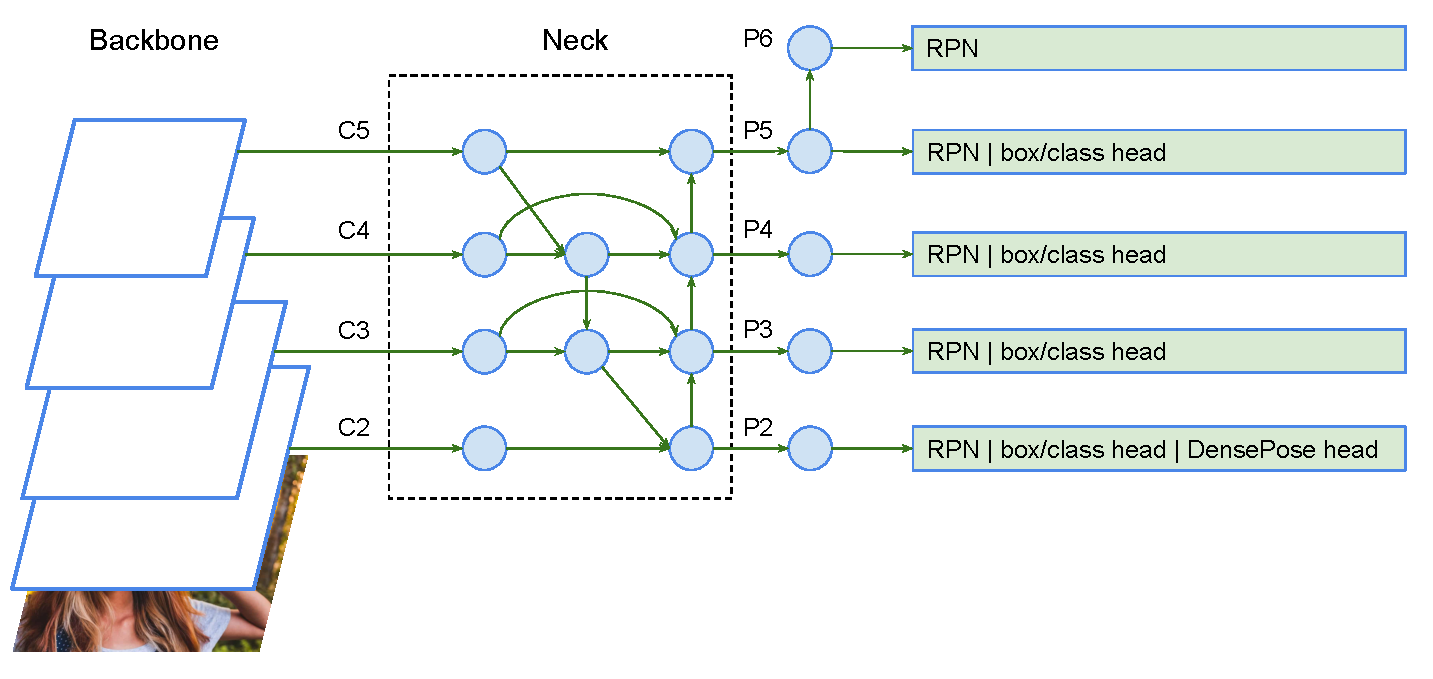
\includegraphics[width=0.4\textwidth]{images/scheme.pdf}
\caption{The high level structure of the Mobile Parsing R-CNN model. $C_i$, $P_i$ represent feature levels with a resolution of $1/2^i$ of the input image. $P_6$ is obtained via stride-2 pooling on $P_5$.}
\label{fig:scheme}
\end{figure}
\section{Mobile Parsing R-CNN}
\label{section3}

In this section, we address the design choice of different parts inside our model, which we call Mobile Parsing R-CNN. In general, the model's design follows the Parsing R-CNN model, the winner solution of the COCO 2018 Challenge DensePose Estimation task, but with different modifications in different parts.

\subsection{Backbone}

While there are many different possible designs of a backbone network, we target efficient models with a block structure as that in MobileNetV1 and V2 \cite{mobilenetv1, mobilenetv2} (depth-wise separable convolutions and inverted residuals with linear bottlenecks). This base block is the foundation for most efficient backbones used today, which were selected for evaluation as the backbone of the improved model. 
Let us list various architectures we use in our experiments:
\begin{itemize}
    \item \textbf{MobileNetV3}.  \cite{mobilenetv3} applies neural architecture search (NAS) and improves MobileNetV2 by adopting Squeeze and excitation block for channel-wise attention and non-linearities like h-sigmoid and h-swish;
    \item \textbf{MixNet}. \cite{mixnet} develops a multi-kernel variant of MobileNetV2, i.e., depth-wise convolutions consisting of convolutions with different kernel sizes;
    \item \textbf{Differentiable NAS} considers the problem of finding neural architecture in a differentiable way by carefully designing search space. We consider the following models, obtained using the differentiable NAS procedure: MnasNet \cite{mnasnet}, FBNet \cite{fbnet}, Single-Path\cite{spnasnet};
    \item \textbf{EfficientNets} from \cite{efficientnetb} appear to be one of the first architectures, obtained using AutoML approaches for image classification, and achieve a good compromise between the accuracy on a classification task and the number of the parameters of the network. \cite{efficientnetb} shows that one can apply a power-law scaling of width as a function of depth. Later EfficientNets were customized for Google's Edge TPUs \cite{efficientnete} using MNAS framework \cite{mnasnet};
    \item \textbf{CondConv}. Traditional convolutional layers have the kernel weights fixed once they are trained. CondConv \cite{condconv} applies a linear combination of several kernels (a mixture of experts) with weights generated dynamically by another network based on the input. While the original work is devoted to the classification task, we explore this \textit{``dynamic''} approach combined with EfficientNets on the DensePose task.
\end{itemize}

\subsection{Neck}

The main challenge in the object detection pipeline is to be able to detect objects of different scales. Earlier detectors predict objects based on features extracted from different levels of the backbone. Later, feature pyramid network (FPN \cite{fpn}) proposes to integrate features in a top-down manner to enrich fine-grained features from the lowest level of feature pyramid with semantically rich information from deeper layers. While the original work \cite{fpn} considers only the top-down pathway for information aggregation, later works also add cross-scale connections between the feature levels. In this work, we make use of bidirectional FPN (BiFPN \cite{bifpn}) for multi-scale feature fusion, which outperforms its recent counterparts in object detection tasks (see \cite{bifpn}), while remaining light-weight and fast. It is partly achieved by using separable convolutions inside.

\subsection{Densepose head}

We increase the region of interest (RoI) resolution for the DensePose head from $14\times14$ to $32\times32$, as it was suggested in \cite{parsing}.

While the original network uses 8 convolutions layers in the DensePose head, we, instead, similar to \cite{parsing}, use the atrous spatial pyramid pooling (ASPP) \cite{aspp} module, followed by 4 convolutional layers. Also, we omit the non-local convolutional layer \cite{nonlocal} between ASPP and convolutional layers in order not to increase the latency of the network because it performs pixel to pixel comparisons resulting in $O(n^2)$ operations, where $n$ is the number of pixels.

Finally, the DensePose predictions happen on the finest level from the feature pyramid as in \cite{parsing}, while box/class predictions happen on all levels.

\subsection{Quantization of backbone layers}
\label{quant}

We proposed the quantization procedure for Parsing R-CNN based on quantization aware training tools provided by PyTorch. 
First of all, it is necessary to patch the existing network architecture. Considering the whole network operates with quantized tensors, we should find intermediate parts where floating-point tensors are crucial to obtain satisfactory results.
\begin{enumerate}
    \item RPN classification and regression heads use a $3\times3$ convolutional layer to produce a shared hidden state from which one $1\times1$ convolutional layer predicts objectness logits for each anchor, and another one predicts bounding-box deltas specifying how to refine the anchor coordinates to get a final object proposal. These layers work with quantized feature tensors, but for correct calculation of RPN proposals, predicted objectness logits and anchor deltas are dequantized after inference of bounding box predictor.
    \item To perform accurate RoI pooling, it is necessary first to dequantize input features, apply pooling, and then quantize features back.
    % \item To perform accurate box pooling, it is necessary to dequantize input features. In that case, RoI pooling would work with floating-point features and RPN proposals. After this operation, we quantize cropped feature tensors before passing them to the following layers.
\end{enumerate}

The second step is fusion. We fuse each convolutional and linear layer, followed by batch normalization and activation to one atomic layer. That is needed to save on memory access while also improving the operations' numerical accuracy.
The third step is to run the quantization aware training of the patched and fused model.
% The last step is to perform an evaluation of the resulted model.

During the second and third steps, we run into design obstacles that are described below.

In BiFPN architecture, we collect features before point-wise linear convolutions using pre-forward hooks. This allows us to link to this layer's input rather than to the output of the input provider. But quantization tools implemented in the PyTorch framework at this stage do not allow this to be done. We proposed a mechanism that preserves pre- and post- forward hooks during fusion and preparation for quantization and does not harm the quality of the quantization process itself. The diagram of the proposed mechanism is in Fig.~\ref{fig:preserve_hooks}.

\begin{figure}[!hbtp]
\centering
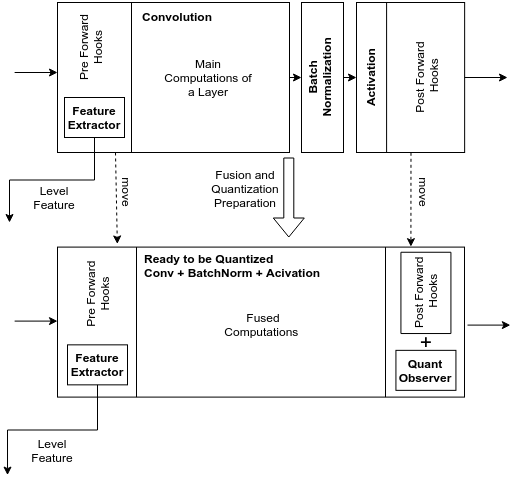
\includegraphics[width=0.4\textwidth]{Figures/densepose/diagram.png}
\caption{The feature collection scheme for quantized models.}
\label{fig:preserve_hooks}
\end{figure}
\section{Experiments}

In this section, we provide the experimental results on design choices for different parts of the model. The majority of experiments are done on the cluster, and finally, we transfer the model to a mobile device to check the performance there.

\subsection{Implementation details}

The models were implemented in PyTorch using Detectron2 \cite{detectron2} platform.

We choose hyper-parameters matching to those in Parsing R-CNN\cite{parsing}, i.e., we use a batch of 16 images (2 images per GPU), therefore we apply synchronous batch normalization \cite{syncbn} instead of usual batch normalization wherever it is used inside the backbone and neck. We use no normalization in box/class and dense pose heads. We sample 512 RoIs for box/class head and 32 RoIs for dense pose head. By default, we train models for 130k iterations with initial learning rate 0.002, decreasing it by 10 at 100k and 120k iterations. Under such a schedule, training of one model takes approximately 1 day on 8 NVIDIA Tesla V100 GPUs. Since all models are quite small, the memory consumption during training allows to decrease the number of GPUs for parallel training. Unless specified otherwise, by default, we scale images in a way that shortest image size equals 800 pixels during the inference stage. Each model's backbone is initialized with weights of the corresponding network trained on the ImageNet classification task. We train models on a combination of \textit{train} and \textit{valminusminival} partitions of Densepose-COCO dataset \cite{densepose} and test them on a \textit{minival} partition.


\subsection{Metrics}
Following the original work, we use as evaluation metric the Average Precision (AP) at a number of \textit{geodesic point similarity} (GPS) thresholds ranging from 0.5 to 0.95. We also report box average precision.

As we are interested in deploying a DensePose model on a mobile device, we report the number of parameters of each model and FPS measured on CPU and GPU. In particular, we measure the inference performance of all models on the same NVIDIA GeForce GTX 1080 Ti. It is worth mentioning that the DensePose model is a two-stage model, so the FPS of the model is directly conditioned on the performance of the first stage of the model. There is a subtle trade-off between the quality and latency; as for example, the network that does not predict any instances will never run dense pose head, and vice versa, the network that produces many false-positive results would redundantly run the model heads. As the latency of the network is data-dependent, we average latency time across DensePose-COCO minival dataset and finally convert it to FPS.

\subsection{Ablation on components}

\begin{table*}[t!]
\centering
\resizebox{\textwidth}{!}{
\begin{tabular}{cllll}
 &  DensePose R-CNN (baseline) \cite{densepose} & Parsing R-CNN \cite{parsing} & Mobile Parsing R-CNN (A) & Mobile Parsing R-CNN (B) \\\hline
Backbone & ResNet-50 \cite{resnet} & ResNet-50 \cite{resnet} & Single-Path \cite{spnasnet} & Single-Path \cite{spnasnet} \\
Neck & FPN\cite{fpn} & FPN\cite{fpn} & FPN\cite{fpn} & BiFPN  \\
RoI resolution & $14\times14$ & $32\times32$ & $32\times32$ & $32\times32$ \\
Pooling Type & RoIPool & RoIPool & RoIAlign & RoIAlign \\
Box/class head & 2 linear layers & 2 linear layers & 2 conv layers & 2 conv layers \\
% test time shortest image size & 800px & 800px & 800px & 800 px\\
Feature level for prediction & $P_2$,$P_3$,$P_4$,$P_5$ & $P_2$ & $P_2$ & $P_2$ \\
DensePose head & 8 conv layers & ASPP\cite{aspp}+NL\cite{nonlocal}+4 conv layers & ASPP\cite{aspp}+4 conv layers & ASPP\cite{aspp}+4 conv layers \\
\#Channels & 512 & 512 & 256 & 64 \\
\hline
\#Params & 59.73M & 54.36M & 11.35M & 3.35M \\
GPU FPS & $13.16$ & $10.15$ & $12.03$ & $22.77$ (3x LR: $\mathbf{23.55}$) \\
CPU FPS & $1.62$ & $1.39$ & $1.42$ & $2.02$  (3x LR: $\mathbf{2.10}$) \\
box AP & $57.8$ & $59.609$ & $56.370$ & $55.39$ (3x LR: $56.83$)\\
densepose AP & $49.8$ & $54.676$ & $49.512$ & $46.79$ (3x LR: $51.08$)\\
\hline
\end{tabular}}
\caption{The main differences between the models presented. Results on DensePose-COCO minival. 3x LR refers to 3 times longer training compared to the default setting. $P_i$ represents a feature level with a resolution of $1/2^i$ of the input images. \#Channels represent the number channels inside \textit{neck} and \textit{heads}.}
\label{table:configs}
\end{table*}

% TODO describe testing pipeline

% In this section we show how we accelerated Parsing R-CNN architecture for dense pose estimation task.

% TODO highlight the differences 
\begin{table*}[t!]
\centering
\resizebox{\textwidth}{!}{
\begin{tabular}{lcccccc}
\hline
Backbone & Top-1 Accuracy (\%) & \#Params & box AP & dp. AP & GPU FPS & CPU FPS \\ \hline
ResNet-50 \cite{resnet} & $77.15$ & $33.61$M & $60.0$ & $\mathbf{54.7}$ & $11.05$ & $1.34$ \\
EfficientNet-B3 \cite{efficientnetb} & $81.636$ & $16.03$M & $59.027$ & $53.084$ & $8.31$ & $1.37$ \\
EfficientNet-EdgeTPU-L \cite{efficientnete} & $80.534$ & $17.89$M & $60.069$ & $53.378$ & $8.11$  & $1.34$ \\
MixNet-XL \cite{mixnet} & $80.120$ & $19.10$M & $58.444$ & $51.475$ & $8.54$  & $1.32$ \\
EfficientNet-B2 \cite{efficientnetb} & $79.688$ & $13.68$M & $58.041$ & $51.800$ & $9.33$ & $1.38$ \\
MixNet-L \cite{mixnet} & $78.976$ & $14.62$M & $57.481$ & $50.649$ & $8.52$ & $1.34$ \\
EfficientNet-EdgeTPU-M \cite{efficientnete} & $78.742$ & $14.57$M & $58.825$ & $52.302$ & $9.21$ & $1.37$ \\
EfficientNet-B1 \cite{efficientnetb} & $78.692$ & $13.03$M & $57.654$ & $51.053$ & $9.49$ & $1.39$ \\
CondConv-EfficientNet-B0 \cite{efficientnete, condconv} & $77.304$ & $18.32$M & $56.779$ & $49.231$ & $10.63$ & $1.40$ \\
EfficientNet-EdgeTPU-S \cite{efficientnete} & $77.264$ & $13.12$M & $58.296$ & $51.606$ & $10.03$ & $1.39$ \\
MixNet-M \cite{mixnet} & $77.256$ & $12.39$M & $56.834$ & $48.371$ & $9.39$ & $1.35$ \\
EfficientNet-B0 \cite{efficientnetb} & $76.912$ & $12.10$M & $56.271$ & $49.647$ & $10.53$ & $1.39$ \\
MixNet-S \cite{mixnet} & $75.988$ & $11.52$M & $55.132$ & $46.685$ & $10.34$ & $1.37$ \\
MobileNetV3-Large-1.0 \cite{mobilenetv3} & $75.516$ & $12.04$M & $54.537$ & $47.195$ & $11.54$ & $1.40$ \\
MnasNet-A1 \cite{mixnet} & $75.448$ & $10.94$M & $54.648$ & $47.036$ & $11.21$ & $1.38$ \\
FBNet-C \cite{fbnet} & $75.124$ & $11.49$M & $55.399$ & $47.983$ & $10.97$ & $1.37$ \\
MnasNet-B1 \cite{mnasnet} & $74.658$ & $11.31$M & $52.280$ & $47.658$ & $11.24$ & $1.37$ \\
Single-Path \cite{spnasnet} & $74.084$ & $11.35$M & $56.370$ & $49.512$ & $\mathbf{12.03}$ & $\mathbf{1.42}$ \\
MobileNetV3-Large-0.75 \cite{mobilenetv3} & $73.442$ & $10.92$M & $52.763$ & $44.736$ & $11.02$ & $1.36$ \\
MobileNetV3-Large-1.0 (minimal) \cite{mobilenetv3} & $72.244$ & $10.48$M & $52.464$ & $44.632$ & $11.33$ & $1.36$ \\
MobileNetV3-Small-1.0 \cite{mobilenetv3} & $67.918$ & $10.07$M & $49.614$ & $35.808$ & $10.62$ & $1.35$ \\
MobileNetV3-Small-0.75 \cite{mobilenetv3} & $65.718$ & $9.74$M & $44.224$ & $32.650$ & $10.16$ & $1.33$ \\
MobileNetV3-Small-1.0 (minimal) \cite{mobilenetv3} & $62.898$ & $9.58$M & $45.989$ & $36.522$ & $10.34$ & $1.34$ \\\hline
\end{tabular}}
\caption{Ablation on the backbone network used in Mobile Parsing R-CNN (A). The backbones are sorted by top-1 accuracy. Results on DensePose-COCO \textit{minival}}
\label{table:backbones}
\end{table*}

First, we implemented the Parsing R-CNN \cite{parsing} in Detectron2 following the original implementation. Then we modify the architecture exploiting the techniques presented in the Section~\ref{section3} and present two versions of a new model: Mobile Parsing R-CNN (A) and Mobile Parsing R-CNN (B). See the main architecture differences and obtained results in Table~\ref{table:configs}. Parsing R-CNN outperforms the baseline DensePose R-CNN model by $4.9$ AP, while the Mobile Parsing R-CNN (A) becomes more light-weight with the densepose AP similar to that achieved by the baseline model. The qualitative comparison can be seen in Fig.~\ref{fig:fconfigs}.

Specifically, Mobile Parsing R-CNN (A) is evolved from Parsing R-CNN by careful choice of a backbone, removing non-local block \cite{nonlocal}, decreasing the number of channels in FPN and all heads. Finally, we replace linear layers with convolutional ones in a box/class head. The results of a backbone comparison for Mobile Parsing R-CNN (A) can be seen in Table~\ref{table:backbones}. We use the backbones pretrained on ImageNet from \cite{geffnet}. First, we see that ResNet-50 provides a solid baseline both in terms of AP and FPS. The good FPS can be explained by the fact that the ResNet-50 is one of the first widespread popular deep networks, and GPU manufacturers constantly include this model for bench-marking. In the meantime, other networks contain specific new custom layers and are mainly designed for mobile or embedded devices. Nevertheless, by analyzing results in the Table~\ref{table:backbones}, we pick the Single-Path \cite{spnasnet} backbone as a network providing a good balance between FPS and the dense pose AP.

We move on from Mobile Parsing R-CNN (A) to Mobile Parsing R-CNN (B), by introducing a  new feature aggregation module (BiFPN \cite{bifpn} instead of FPN \cite{fpn}) and further decreasing the number of channels in the dense pose head by a factor of 4, thus 8 times lower than in the baseline architecture. The individual effects of each change can be found in Table~\ref{table:channels}. The transfer from FPN to BiFPN results in a reduced number of parameters,  better box, and densepose AP and the identical FPS. The $4\times$ decrease of the number of channels in BiFPN and all heads results only in $6.0$ densepose AP reduction, while increasing FPS approximately $2$ times.


Our implementation of BiFPN differs from the original one in terms of up-sampling and down-sampling procedure type used to make features from different levels of backbone spatially compatible for the fusion. While the original work uses a bilinear (up)down-sampling, we use a nearest-neighbor variant since we found it to be much faster on mobile devices, and the drop in AP is very slight. Also, in the case of BiFPN, we use features before point-wise linear $1\times1$ convolutions, compared to ``after'' in case of FPN, as it results in slight improvement of dense pose AP. Finally, we train the model three times more iterations, i.e., 390k iterations, reducing learning rate by 10 at 330k and 370k iterations and call it Mobile Parsing R-CNN (B s3x).

\begin{table*}[t!]
\centering
\resizebox{0.8\textwidth}{!}{
\begin{tabular}{cccccccc}
\hline
 & Neck & \#channels & \#Params & box AP & dp. AP & GPU FPS & CPU FPS  \\\hline
Mobile Parsing R-CNN (A) & FPN & $256$ & $11.35$M & $56.371$ & $49.512$ & $12.03$ & $1.42$ \\
 & BiFPN & $256$ & $10.53$M & $58.106$ & $52.80$ & $12.05$ & $1.41$ \\
& BiFPN & $112$ & $4.41$M & $56.41$ & $49.64$ & $19.04$ & $1.78$ \\
& BiFPN & $88$ & $3.82$M & $56.08$ & $48.19$ & $20.43$ & $1.87$ \\
Mobile Parsing R-CNN (B) & BiFPN & $64$ & $3.35$M & $55.39$ & $46.79$ & $22.77$ & $2.02$ \\\hline
\end{tabular}}
\caption{Ablation on neck type and number of channels. The number of channels is the same in neck and heads. Results on DensePose-COCO \textit{minival}}
\label{table:channels}
\end{table*}

% TODO: somehow highlite the differences or move to appendix
\begin{figure*}[t!]
\centering
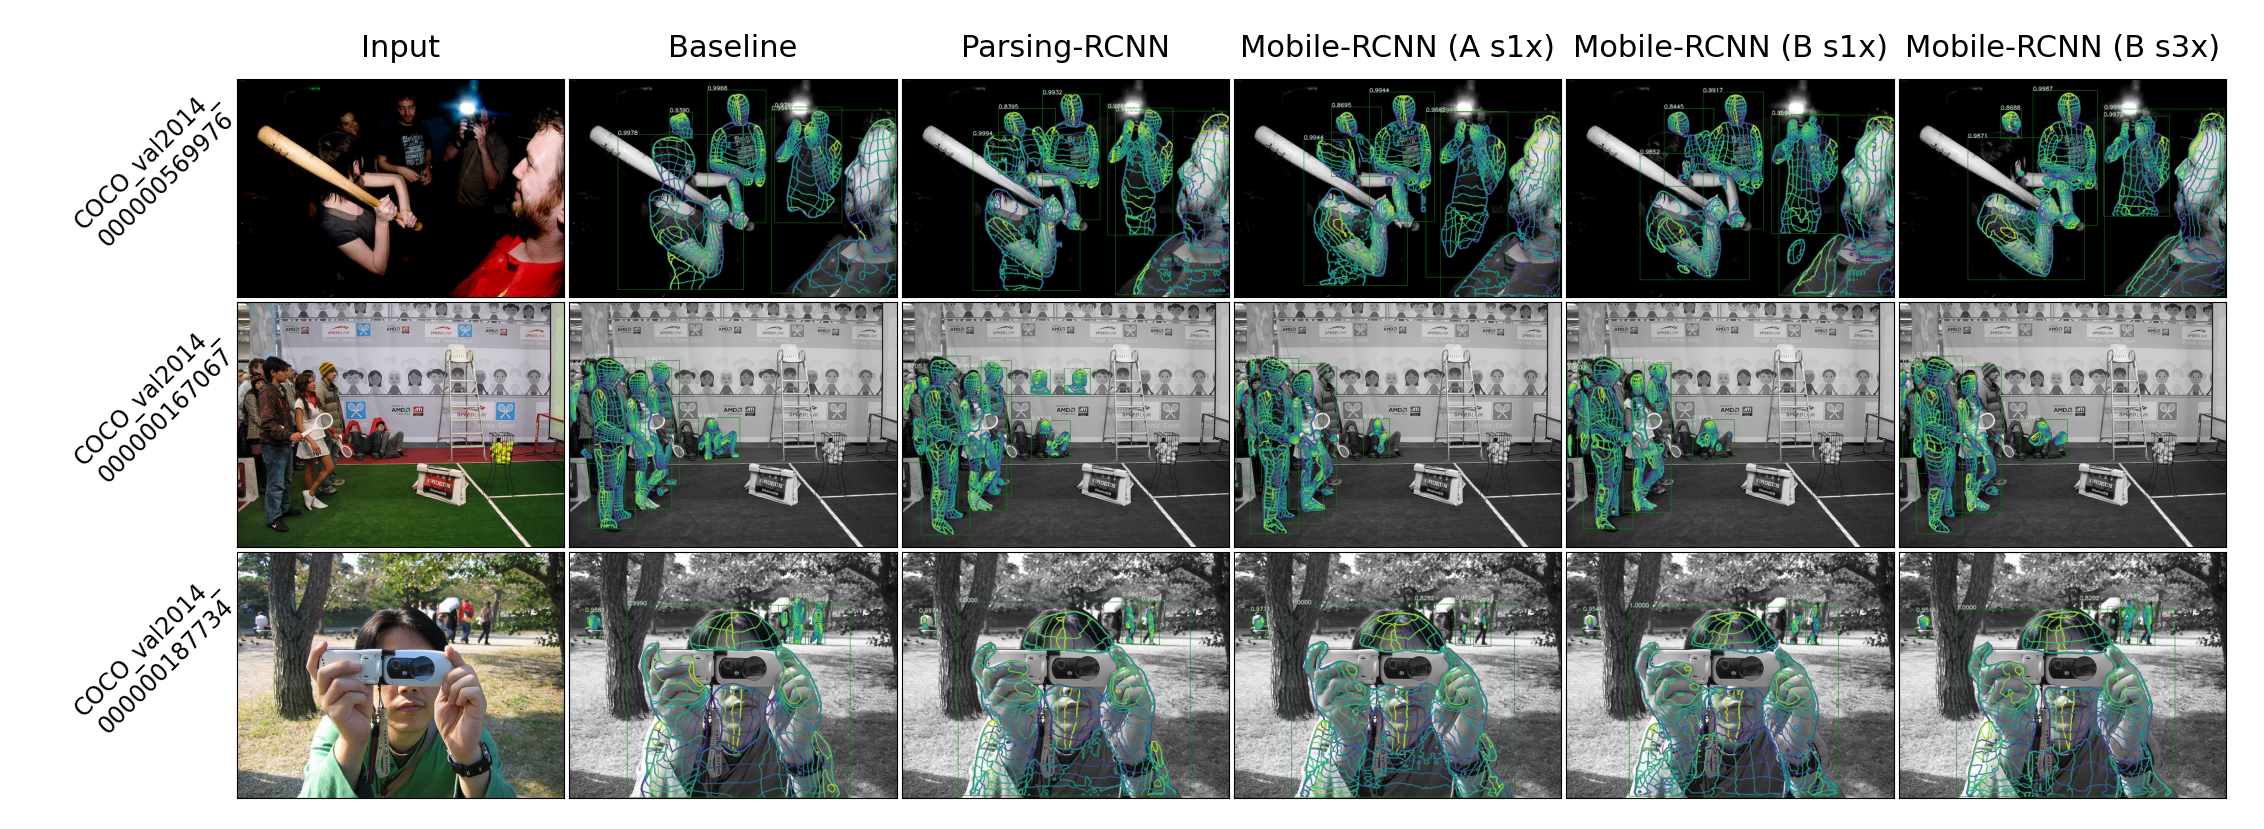
\includegraphics[width=0.9\textwidth]{Figures/densepose/qconfigs_decr.png}
\caption{Qualitative comparison of different models. We depict contours with color-coded U and V coordinates as an output of the model.}
\label{fig:fconfigs}
\end{figure*}

\begin{figure*}[t!]
\centering
\includegraphics[width=0.8\textwidth]{Figures/densepose/mob_comp2.png}
\caption{Qualitative comparison of different backends. We depict contours with color-coded U and V coordinates as an output of the model.}
\label{fig:configs}
\end{figure*}

\subsection{Smartphone-based implementation}


\begin{table*}[t!]
\centering
\resizebox{0.8\textwidth}{!}{
\begin{tabular}{cccccc}
\hline
image shortest side & box AP & dp. AP & GPU FPS & CPU FPS & mobile CPU FPS\\\hline
200px & 36.449 & 19.028 & 27.549 & 10.277 & 2.355\\
400px & 49.181 & 43.916 & 24.648 & 6.921 & 0.954\\
512px & 51.709 & 47.887 & 26.970 & 4.976 & 0.640\\
600px & 53.423 & 49.675 & 25.669 & 4.290 & 0.498\\
800px & 54.744 & 50.560 & 24.033 & 3.046 & N/A\\
1000px & 55.163 & 49.466 & 20.061 & 2.071 & N/A\\\hline
\end{tabular}}
\caption{The impact of image size. Results are obtained with Mobile Parsing R-CNN (B s3x, test-tuned) on DensePose-COCO \textit{minival}. The N/A values correspond to tensor sizes that produced errors on mobile device}
\label{table:pixel}
\end{table*}

\begin{table*}[t!]
\centering
\resizebox{0.9\textwidth}{!}{
\begin{tabular}{ccccccccccc}
\hline
max \# of people & box AP & box APs & box APm & box APl & dp. AP & dp. APm & dp. APl & GPU FPS & CPU FPS & mobile CPU FPS\\\hline
1 & 83.110 & - & 83.389 & 83.173 & 54.329 & 48.203 & 54.765 & 27.508 & 5.859 & 0.684 \\
2 & 74.700 & 24.058 & 56.672 & 77.359 & 52.402 & 47.694 & 52.991 & 27.729 & 5.626 & 0.664 \\
3 & 71.508  & 16.357 & 54.621 & 76.280 & 52.324 & 47.973 & 52.905 & 26.767 & 5.584 & 0.638 \\
4 & 68.818 & 19.532 & 52.693 & 75.693 & 52.050 & 43.131 & 52.838 & 27.198 & 5.510 & 0.606 \\
5 & 66.756 & 20.252 & 53.543 & 74.807 & 51.468 & 44.154 & 52.501 & 27.732 & 5.443 & 0.603 \\\hline
\end{tabular}}
\caption{The impact of number of people in the frame on performance characteristics. Results are obtained with Mobile Parsing R-CNN (B s3x, test-tuned) on DensePose-COCO \textit{minival}. The shortest image side is 512 pixels}
\label{table:people}
\end{table*}

We evaluate the mobile model with Caffe2 runtime, running on a smartphone with ARM processor with 8 cores, 8 threads, and the highest core clock of 2600 MHz.

We use the deployment conversion tools provided by Detectron2 \cite{detectron2}. Specifically, the network is transferred first to ONNX format, then to Caffe2 format.

% \textbf{MODEL.RPN.POST_NMS_TOPK_TEST 100 MODEL.ROI_HEADS.NMS_THRESH_TEST 0.3}
In general, two-stage models introduce numerous hyper-parameters. In case of test-time hyper-parameters, we found empirically, among many different options, that choosing $100$ instead of $1000$ region proposals per \textit{neck} level after non-maximum suppression (NMS) in RPN and changing IoU threshold in NMS from $0.5$ to $0.3$ leads to a significant boost of the model. Therefore later, we use this setup of the model and call it Mobile Parsing R-CNN (B s3x test-tuned).

We check the impact of the image size on the model (see Table~\ref{table:pixel}). The lower resolution of the image, the faster inference we get, but the reduction of image size results in a reduction of densepose AP. In the case of mobile inference, we apply the model on images with the shortest side of size 512 pixels, because it is the lowest resolution processed by the model during the training phase.


% TODO put a number on % of images with less than 5 people 
We are mostly interested in practical applications on the end-device with data fed straight from the device's camera. In this case, usually, the limited number of people appears in the frame. We test the model performance on filtered versions of COCO-DensePose minival partition, where the filtering is based on the maximum number of people in the image. The results can be seen in Table~\ref{table:people}. One can see that the fewer people are in the image, the better performance of the model in AP and FPS. Usually, the fewer people in the image, the more area each person occupies in the frame, which leads to more accurate predictions.

\subsection{Model quantization results}

Here we report the performance statistics of the model obtained using the quantization approach described in Section~\ref{quant}. Thanks to the quantization, we increased the speed of inference by a factor of two and decreased the model size by a factor of three. See exact values in Table~\ref{table:quant}.


\begin{table}[!t]
\centering
\resizebox{0.4\textwidth}{!}{
\begin{tabular}{cccccc}
\hline
weights type & model size & dp. AP & CPU FPS \\\hline
float32 & 13.8mb & 47.887 & 4.976 & \\
int8 & 4.3mb & 44.033 & 8.310 & \\\hline
\end{tabular}}
\caption{The effect of quantization. Results are obtained with Mobile Parsing R-CNN (B s3x, test-tuned) on DensePose-COCO minival. The shortest image side is 512 pixels}
\label{table:quant}
\end{table}
\section{Conclusion}

In this work we showed that it is possible to significantly compress and speed up models ($17\times$ model size reduction and $2\times$ latency improvement) for DensePose estimation task utilizing existing state-of-the-art solutions of this task's subproblems, achieving a good balance between speed, model size and average precision of the model. In the process, we performed an ablation study of 23 different backbones and detection pipeline characteristics, particularly applied for the DensePose task.
By optimizing different parts of R-CNN-like models, we achieved significant performance improvement compared to the baseline model.
We performed deployment of the final model to the mobile device, measured its performance, and discovered factors affecting it. 
The proposed architecture Mobile Parsing R-CNN is both fast and light-weight. Notably, the final model weighs 13.8MB and runs near real-time $\sim27$ FPS on Nvidia Tesla 1080Ti GPU, and $\sim1$ FPS on a mobile device using the only CPU. Using a runtime environment that utilizes mobile GPU or Neural Network acceleration hardware (NPUs), it would be trivial to get near-real-time performance on a mobile phone.
\newline\newline
\noindent\textbf{Acknowledgment.} The authors acknowledge the usage of the Skoltech CDISE HPC cluster Zhores for obtaining the results presented in this paper. This work was supported partially by the Ministry of Education and Science of the Russian Federation (Grant no. 14.756.31.0001).

%\FloatBarrier

% {\small
% \bibliographystyle{ieee_fullname}
% \bibliography{egbib}
% }

% \end{document}

\newpage
% \documentclass{article}

% if you need to pass options to natbib, use, e.g.:
%     \PassOptionsToPackage{numbers, compress}{natbib}
% before loading neurips_2020

% ready for submission
% \usepackage{neurips_2020}

% to compile a preprint version, e.g., for submission to arXiv, add add the
% [preprint] option:
% \usepackage[nonatbib,final]{neurips_2020}
%\usepackage[nonatbib,preprint]{neurips_2020}

% to compile a camera-ready version, add the [final] option, e.g.:
%     \usepackage[final]{neurips_2020}

% to avoid loading the natbib package, add option nonatbib:
% \usepackage[nonatbib]{neurips_2020}

% \usepackage[utf8]{inputenc} % allow utf-8 input
% \usepackage[T1]{fontenc}    % use 8-bit T1 fonts
% % \usepackage[T2A]{fontenc}
% \usepackage{hyperref}       % hyperlinks
% \usepackage{url}            % simple URL typesetting
% \usepackage{booktabs}       % professional-quality tables
% \usepackage{amsfonts}       % blackboard math symbols
% \usepackage{nicefrac}       % compact symbols for 1/2, etc.
% \usepackage{microtype}      % microtypography

% \usepackage{comment}
% \usepackage{graphicx}
% \usepackage{amsmath,amssymb} % define this before the line numbering.
% \usepackage{color}
% % \usepackage[width=122mm,left=12mm,paperwidth=146mm,height=193mm,top=12mm,paperheight=217mm]{geometry}
% % \usepackage{cmap}					% поиск в PDF
% \usepackage[english]{babel}	% локализация и переносы
% % \usepackage[english,russian]{babel}
% \usepackage{wrapfig}

% \usepackage{booktabs, multirow} % for borders and merged ranges
% \usepackage{soul} % for underlines
% \usepackage[table,dvipsnames]{xcolor} % for cell colors
% \usepackage{changepage,threeparttable} % for wide tables

% \usepackage[export]{adjustbox}
% \usepackage{xfrac}
% \usepackage{wrapfig}

% % \usepackage[dvipsnames]{xcolor}
% \newcommand{\lat}{\selectlanguage{english}}

% % \iftoggle{nocomments}{
% % 	\newcommand{\DZ}[1]{\ignorespaces}
% % 	\newcommand{\EB}[1]{\ignorespaces}
% % 	\newcommand{\OV}[1]{\ignorespaces}
% % 	\newcommand{\LA}[1]{\ignorespaces}
% % 	\newcommand{\VE}[1]{\ignorespaces}
% % 	\newcommand{\DV}[1]{\ignorespaces}
% % 	\newcommand{\todo}[1]{\ignorespaces}
% % 	\newcommand{\todoshort}[1]{\ignorespaces}
% % }{
% % }

% \newcommand{\MATTHIAS}[1]{\textcolor{red}{\textbf{Matthias: #1}}}
% \newcommand{\DZ}[1]{\textcolor{ForestGreen}{DZ: #1}}
% \newcommand{\EB}[1]{\textcolor{magenta}{EB: #1}}
% \newcommand{\AN}[1]{\textcolor{orange}{AN: #1}}
% \newcommand{\LA}[1]{\textcolor{Plum}{\textbf{AA: #1}}}
% \newcommand{\VI}[1]{\textcolor{blue}{VI: #1}}
% \newcommand{\DV}[1]{\textcolor{Sepia}{DV: #1}}
% \newcommand{\todo}[1]{\textcolor{red}{TODO: #1}}
% \newcommand{\todoshort}[1]{\textcolor{red}{#1}}

% \DeclareMathOperator*{\argmax}{arg\,max}
% \DeclareMathOperator*{\argmin}{arg\,min}


% \title{Scan2Part: Part Segmentation of~Real-World 3D~Scenes}
\chapter{Scan2Part: Part Segmentation of~Real-World 3D~Scenes}



% The \author macro works with any number of authors. There are two commands
% used to separate the names and addresses of multiple authors: \And and \AND.
%
% Using \And between authors leaves it to LaTeX to determine where to break the
% lines. Using \AND forces a line break at that point. So, if LaTeX puts 3 of 4
% authors names on the first line, and the last on the second line, try using
% \AND instead of \And before the third author name.

% \author{
%     Alexandr Notchenko , Vladislav Ishimtsev , Evgeny Burnaev\\
%   \texttt{\{a.notchenko,v.ishimtsev,e.burnaev\}@skoltech.ru} \\
% Skolkovo Institute of Science and Technology \\
% }
% \author{%
%   David S.~Hippocampus\thanks{Use footnote for providing further information
%     about author (webpage, alternative address)---\emph{not} for acknowledging
%     funding agencies.} \\
%   Department of Computer Science\\
%   Cranberry-Lemon University\\
%   Pittsburgh, PA 15213 \\
%   \texttt{hippo@cs.cranberry-lemon.edu} \\
  % examples of more authors
  % \And
  % Coauthor \\
  % Affiliation \\
  % Address \\
  % \texttt{email} \\
  % \AND
  % Coauthor \\
  % Affiliation \\
  % Address \\
  % \texttt{email} \\
  % \And
  % Coauthor \\
  % Affiliation \\
  % Address \\
  % \texttt{email} \\
  % \And
  % Coauthor \\
  % Affiliation \\
  % Address \\
  % \texttt{email} \\
% }

% \begin{document}
% \maketitle

% \begin{abstract}
% In this paper, we explore the part taxonomies of objects in indoor scenes and their effect on scene understanding and reconstruction models. To do that we introduce the problem of real-world 3D scene part segmentation. To help us design a benchmark for this problem, we introduce a new dataset titled "Scan2Part". Using this dataset, we train models capable of solving the problem of part segmentation for scene data collected with 3D sensors.
 
 
We propose Scan2Part, a method to segment individual parts of objects in real-world, noisy indoor RGB-D scans.
%
To this end, we explore the part taxonomies of objects in indoor scenes and their effect on scene understanding models.
%
Specifically, we propose a new U-Net-based architecture that captures the fine-scale detail of the underlying 3D scan geometry by leveraging a multi-scale feature hierarchy.
%
As output, we are able to predict fine-grained per-object part labels, even when the geometry is coarse or partially missing.
%
In order to train our method, we introduce the Scan2Part dataset, which is the first large-scale effort on real-world scenes providing detailed semantic labels at the part level in the real-world setting.
%
In total, we provide 242,081 correspondences between 53,618 PartNet parts of 2,477 ShapeNet objects and 1,506 Scannet scenes, and we set up a new benchmark with a hidden test set.
%
%Experiments show that method outperforms the best state-of-the-art baseline adopted for this task by 6.32\% mIoU.
%
Overall, we believe that both our method as well as newly introduced dataset is a stepping stone forward towards  structural understanding of real-world 3D environments.

% More ideas:
% 1. In contrast with semantic or instance segmentation tasks, part segmentation is inherently ambiguous for humans. Thus, a way forward for increasing the level of detail may be data-driven part taxonomies.
% 2. These networks, that we propose, are able to jointly learn efficient representations, thus enhancing each other's performance on a number of levels of hierarchy.

%
%Compared to state-of-the-art methods, our network architecture outperforms the best baseline model by 6.32\% mIoU.


\begin{comment}
\vspace{5cm}


\begin{itemize}
    \item We compressed and projected original PartNet taxonomy to Scannet dataset, then pruned it even further depending on class statistics of objects from real-world scenes.
    \item We used segmentation neural network with U-Net with resudual blocks to compute features of voxels.
    \item Using features we predict probabilities of voxel corresponding to instance and semantic labels in the parts taxonomy.
    \item Integrating probabilities of parts to have a better prediction of whole objects and their component parts at the same time.
    \item We an
\end{itemize}


In order to train our method, we a introduce new Scan2Part dataset with 242,081 correspondences between 53,618 PartNet parts of 2,477 ShapeNet objects and 1,506 Scannet scenes. 


Specifically, we introduce the problem of real-world 3D scene part segmentation.  %redundant with first sentence
We introduce a new Scan2Part dataset with 242081 correspondences between 53618 PartNet parts of 2477 ShapeNet objects and 1506 Scannet scenes. 
%
This approach is to training segmentation models of different levels of detail in a joint way while improving the results of each.

% Most of the state of the art research on part segmentation of shapes is performed on Meshes or CAD model datasets, where 3D data modeled through sampling of point clouds or voxelisation, which ignores real-world measurement effects like noise, occlusion and sensor limitations. 

We also explore connections between problems of part instance segmentation, semantic part segmentation, and scene graph inference. We demonstrate how parts taxonomies affect the ability of models to perform segmentation and suggest data-driven approaches to creating new part taxonomies. The models we trained are capable of segmenting scenes into object parts in noisy, heavily occluded environments.
In conclusion, we discuss the limits of applicability of part annotation to raw data measured from sensors and attempting to estimate the best possible performance for part segmentation problem for data with limited resolution and sensor noise.

% \MATTHIAS{Please make bullet points of method here}
% Our method:

% \begin{itemize}
%     \item We compressed and projected original PartNet taxonomy to Scannet dataset, then pruned it even further depending on class statistics of objects from real-world scenes.
%     \item We used segmentation neural network with U-Net with resudual blocks to compute features of voxels.
%     \item Using features we predict probabilities of voxel corresponding to instance and semantic labels in the parts taxonomy.
%     \item Integrating probabilities of parts to have a better prediction of whole objects and their component parts at the same time.
%     \item We analyse prediction errors and suggest an update to a taxonomy so that scene predictions can be more accurate.
% \end{itemize}
\end{comment}

\end{abstract}

\section{Motivation}

%Motivation: RGB-D scanning is here and we want to have a fine-grained understanding of the 3D captures
In the recent years, a wide variety of consumer-grade RGB-D sensors, such as the Intel Real Sense, Microsoft Kinect, depth-sensor enabled smartphones, enabled inexpensive and rapid RGB-D data acquisition. Increasing availability of large, labeled datasets (e.g.,~\cite{chang2017matterport3d,dai2017scannet})  made possible development of deep learning methods for 3D object classification and semantic segmentation. At the same time, acquired 3D data is often incomplete and noisy; while one can identify and segment the objects in the scene, reconstructing high-quality geometry of objects remains a challenging problem.  

An example of the new approach in recent work 
\cite{avetisyan2019scan2cad}, uses a large dataset of clean, labeled geometric shapes
\cite{chang2015shapenet}, for classification/segmentation associating the input point or voxel data with object labels from the dataset, along with adapting geometry to 3D data.  This approach ensures that the output geometry has high quality, and is robust with respect to noise and missing data in the input.  
At the same time, a ``flat'' classification/segmentation approach, with each object in the database corresponding to a separate label and matched to a subpart of the input data corresponding to the whole object, does not scale well as the number of classes grows and often runs into difficulties in the cases of extreme occlusion (only a relatively small part of an object is visible). 
Significant improvements can be achieved by considering object \emph{parts}, or more generally part hierarchies. 
Part-based segmentation of 3D datasets promises to offer a significant improvement both in finding the best matching shape in the dataset, recognizing objects from  highly incomplete data (e.g., from a couple of parts) from  as well as more precise geometry adaptation as well as, potentially, assembly of new shapes out of existing parts yielding a closer match to the input data. 

% large collection of 3D models in database can be reduced to structured representations, 
%objects with occluded sub-parts still can be recognized by parts available in the scan and the rest can be guessed with high probability, using parts, we can reconstruct new objects that are not yet present in the database of shapes. \LA{Whoa: we must either prove this by experiments, or appeal to existing researcg}

%based on different approaches for volumetric information integration, from enhancements of  methods such as volumetric fusion \cite{curless1996volumetric}, to 
%probabilistic  methods, and plethora of methods based on their combinations.

%Compared to computer graphics models manually created by 3D professionals, 3D scans are noisy and incomplete.
% - есть задача восстановления сцен по шумным сканам (всякие слова и ссылки на этот счет были и у нас в статье, и в статьях нисснера про scan2cad)
%Amount of noise and limited resolution of \VI{consumer-grade} consumer grade scanning hardware pose significant challenges for solving this important problem of scene reconstruction. 
%Approaches of reconstruction based on fitting existing 3D assets into scene scans, have shown a lot of promise but still had problems with finding exact models from large database such as ShapeNet \cite{chang2015shapenet}, because of occlusion and lack of spatial context.

% TODO rewrite

%Learning-based approaches are very good at extracting features representative of objects and scenes as a whole, allowing to fill in occluded areas or guess parts affected by noise \cite{dai2017shape,dai2018scancomplete,song2017semantic}. These features are sufficient for scene completion, but they are not as good at recovering geometric primitives like: sharp edges, planar surfaces or borders between sub-parts, resulting in reconstruction quality much poorer than that of 3D content created by humans.

In this work, we focus on the key problem of semantic part segmentation of objects in the scenes, enabling further improvements in  dataset-based reconstruction. 

%\LA{new task: semantic partseg, most parts visible thus apps: nonvisible parts can be inferred, better shape coverage}

In human-made environments, a lot of objects have naturally defined semantic sub-parts, and those sub-parts can, in turn, have their sub-parts, i.e., parts form \emph{hierarchies}.  In our work, we use scene and object representation based on such part hierarchies.  We show how a part-labeled dataset of scanned 3D data suitable for machine learning applications can be constructed, and used to improve the performance of segmentation algorithms. 

%Definitions of sub-parts are based on a set of primitive elements that were manufactured by one formation method or from one material.

%Because of that and the fact that static scenes have other relationships between objects (fixed to each other or in direct surface contact), it's reasonable to suggest a scene description format that possesses a property of hierarchy (e.g., trees or other kinds of graphs).
%We represent scenes as a discrete structures with properties of composability and complex relationships of its parts to compose a whole object and in turn compose a scene from separate objects.
%\LA{usefulness of parts}

%In the last 4 years, the field of computer vision saw an increase in Real-world 3D Scenes datasets acquired using depth sensors and LIDAR's. 
%
%However, due to the limitation of sensors resolution ability, the level of detailization remains the same.
%\DZ{I am not sure this is the reason, and in any case, you need to explain what exactly detailizaiton means in this context}

Our contributions include: 
\begin{enumerate}
\item A new dataset Scan2Part, composed of 1,506 3D reconstructions of real-world scenes with 2,477 aligned 3D CAD models represented by real-world 3D geometry and annotated using hierarchical annotation, which links 3D scene reconstruction with part-annotation of everyday objects.
% \MATTHIAS{highlight stats}
\item We analyze gathered labels and perform compression (aggregation) of instance part taxonomy into hierarchical semantic labels. %\textcolor{blue}{VI: почему 1 и 2 контрибьюшн -- это отдельные пункты, если это всё про 1 датасет}
\item We train multiple models in 3 distinct setups to solve a problem of semantic segmentation of parts in a scene which helps with discovery of new objects and segmentation of objects in the noisy and incomplete geometry of an RGB-D scans. 
%\item 
%\DZ{I would not necessarily make this a separate contribution matbe merge with previous}
%We determined at what detalization level objects loose their unique spacial characteristics and become practically indistinguishable from each other. %\textcolor{blue}{VI: может быть конкретно характеризовать, на каком уровне? типа на уровне разделения объекта на ~10 частей в среднем}
\end{enumerate}

% \textcolor{blue}{VI: создание нового направления сегментации сцены на части}

% \textcolor{blue}{VI: создание пайплайна, которое позволяет улучшить качество обучения высокоуровневых объектов за счёт низкоуровневых объектов}

%\LA{Contributions: 
%* 
%}


% По идее, introduction надо изложить каким-то таким образом (коллеги поправят, если что):
\begin{comment}
\DZ{...I could not follow what the introduction is saying; 
the point of each paragraph is clear but they do not seem to form a coherent story motivating the work;  I can rewrite this, but I'd like to understand first what exactly you had in mind.
\newline
Here is a summary, by paragraph: 
\newline
$\bullet$We have a lot of data now, so reconstruction is important and many methods were developed
\newline
$\bullet$Deep learning was used a lot for segmentation and classification because of reconstruction datasets 
[how do reconstruction datasets help with segmentsaiton/classification? why are we talking about classification/segmentation when we started talking about reconstruction?]
\newline
$\bullet$But more work is needed to use this in real applications
\newline
$\bullet$Reconstruction is difficult because data is noisy, 
one way to solve it is by matching with databases, but this does not always work [ok so back to reconstruction, introducing CAD shape fitting]
\newline
$\bullet$Learning can also extract features which are good for scene completion but not good for geometric primitives
[back to DL again, and features, why do we need these for reconstruction? ]
\newline
$\bullet$We can do better if we solve a new problem of semantic part segmentation: can recognize occluded objects better, 
reconstruct new objects not present in the database. 
Unclear item: large collections can be reduced to new representations
[part segmentation can help to overcome some limitations of CAD shape fitting ]
\newline
$\bullet$ Objects can be naturally made of parts, so scenes need to be described by hierarchies
[seems like a trivial observation but ok, if it were leading somewhere]
\newline
$\bullet$Here are our contributions: (1) dataset collected, (2) compressed 
taxonomy (where did it come from) into hierachical labels,
[never talked about taxonomies yet and we are compressing one all of a sudden] (3) several models tested to do part segmentation helping  (in what sense?) to discover new objects and segment objects in noisy/incomplete data (4) determine what detalization level is too coarse [why is this last thing interesting?]
}
\end{comment}

% \section{Related work}

\noindent 
\textbf{DensePose task.} DensePose-COCO dataset contains a large set of images of people collected ``in the wild'' together with different annotations: (i) bounding boxes, (ii) foreground-background masks, (iii) dense correspondences --- points $p \in S$ of a reference 3D model $S\in\mathbb{R}^3$ of the object associated with triplets $(c, u, v) \in\{1, \ldots, C\} \times[0,1]^{2}$, where $c$ indicates which one of $C$ body parts contains the pixel and $(u,v)$ represents the corresponding location (UV coordinates) in the chart of the part \cite{smpl}.
The DensePose task is then to predict such triplets $(c, u, v)$ for each foreground pixel and every person in the image.
\newline

\noindent \textbf{DensePose R-CNN.} The baseline dense pose prediction model, and all the subsequent works \cite{parsing, uncertainty, monkeys} follow the architecture design of Mask R-CNN \cite{maskrcnn}.

The model is a two-stage: first, it generates class-independent region proposals (boxes), then classifies and refines them using the box/class head. Finally, the DensePose head predicts the body part and UV coordinates for each pixel inside the box. Particularly, the model consists of many different blocks (see Fig.~\ref{fig:scheme}):
\begin{itemize}
    \item \textit{Backbone} to extract features from the image,
    \item \textit{Neck} to integrate features from different feature levels of the backbone to effectively perform multi-scale detection,
    \item \textit{Region proposal network (RPN)} to propose a sparse set of box candidates potentially containing objects,
    \item \textit{Heads} take the features pooled from the bounding box on the corresponding feature level, where the detection occurred, and produce output. The first head is a box/class head, which finally predicts whether the object is present in the box and refines the box coordinates. The second head is the DensePose head that predicts either the pixel belongs to the background or assigns it to one of the 24 DensePose charts, and regresses UV coordinates to each foreground pixel inside the bounding box.
\end{itemize}

\noindent \textbf{Model architecture optimisation.}
In recent years the neural architecture search (NAS) techniques gained popularity \cite{automl}. The main aim of NAS is to find the optimal architecture under specific hardware requirements. Usually, these techniques are applied in simple setups, e.g., classification networks, or in the case of two-stage object detection models, NAS is usually applied to individual parts of the model \cite{nasfpn}. In this paper, instead of creating one more design for a particular part of the model, we try to test different existing approaches and see what works best for the DensePose estimation task. Particularly, we evaluate several backbones that were a result of NAS optimization and try to test them out with other components.

\begin{figure}[!hbtp]
\centering
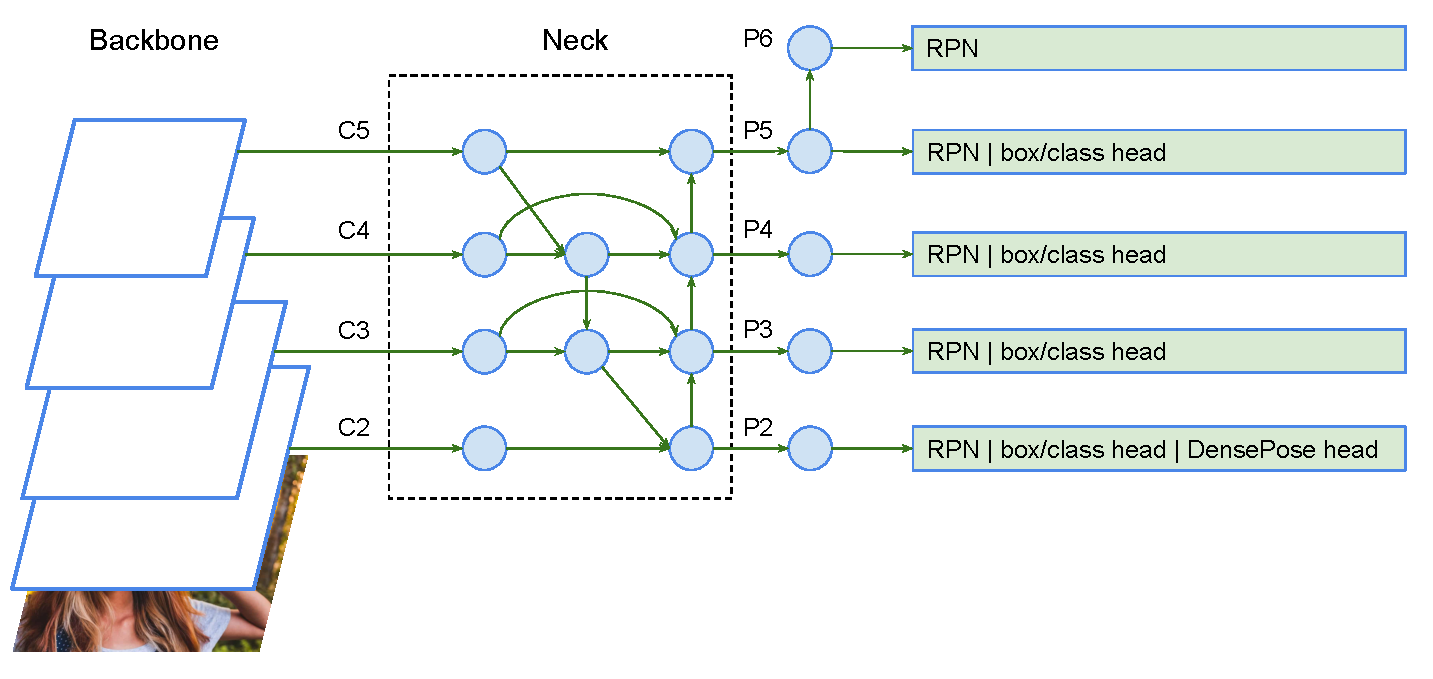
\includegraphics[width=0.4\textwidth]{images/scheme.pdf}
\caption{The high level structure of the Mobile Parsing R-CNN model. $C_i$, $P_i$ represent feature levels with a resolution of $1/2^i$ of the input image. $P_6$ is obtained via stride-2 pooling on $P_5$.}
\label{fig:scheme}
\end{figure}

\section{Dataset}
\label{sec:dataset}

\begin{figure}[!t]
\label{fig:dataset_teaser}
\centering
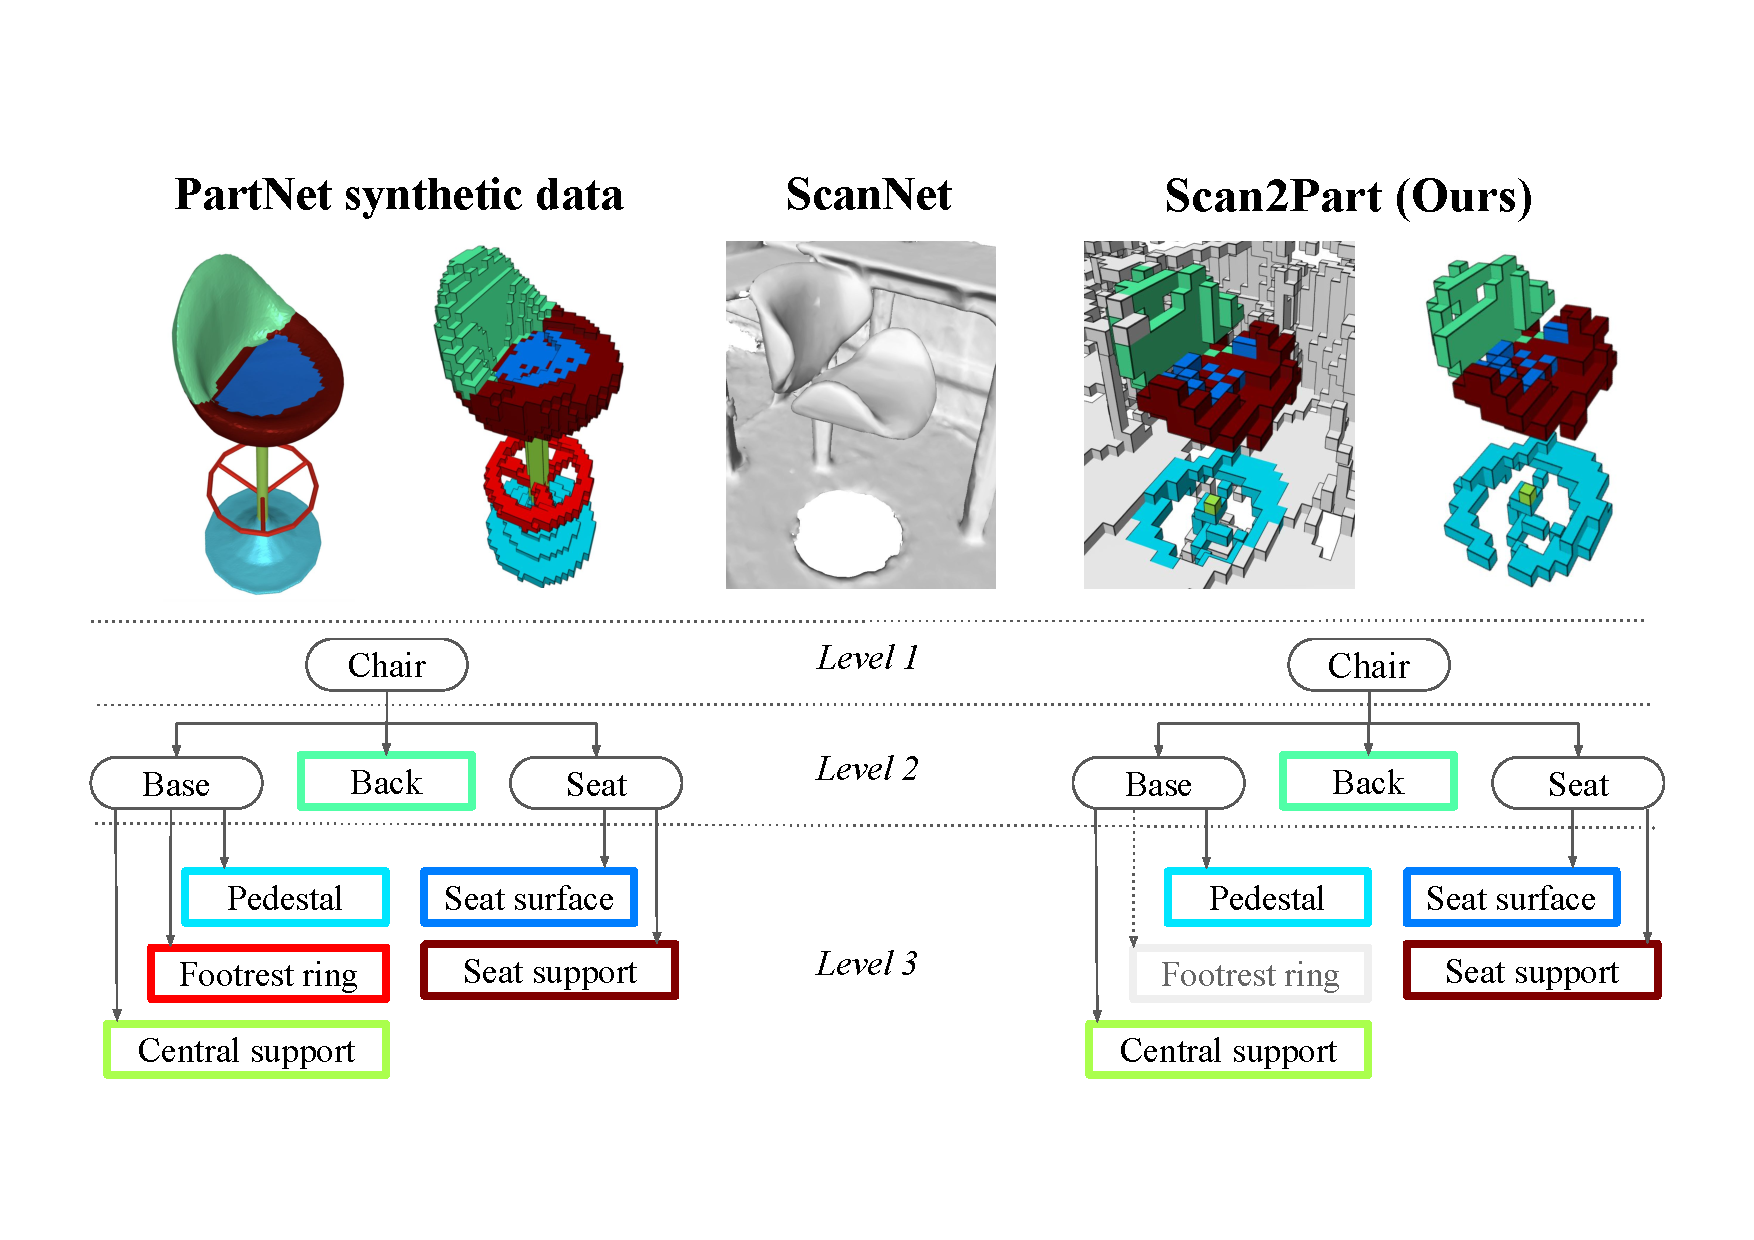
\includegraphics[width=0.99\textwidth]{Figures/scan2part/dataset_teaser.pdf}
\caption{Top:our dataset is obtained by combining PartNet synthetic data with ScanNet sensor data. Bottom: the PartNet object hierarchy is compressed to include only parts sufficiently well represented in ScanNet data.}
\end{figure}

Our first objective is to develop a large-scale 3D scene understanding dataset with part-level annotations. 
We use the 3D geometry in 1,506 3D scenes in ScanNet dataset~\cite{dai2017scannet} reconstructed from RGB-D scans in the form of truncated Signed Distance Function (SDF) at voxel resolution = 3\,cm.
For labeling the scan geometry, we use the parts taxonomy in PartNet dataset~\cite{mo2019partnet} represented as a tree structure where nodes encode parts at various detail levels and edges encode the ``part of'' relationship.
We associate to each 3D scene a per-voxel mask storing leaf part IDs from the taxonomy (i.e., the most fine-grained categories).
To label the 3D scene at a given level~$d$ of semantic detail ($d = 1$ meaning whole objects and $d = 8$ meaning finest parts), we start with the leaf labels in each voxel and traverse the taxonomy tree until hitting depth~$d$.



We further describe the main steps taken to create our Scan2Part benchmark below, leaving the detailed discussion of the technicalities for the supplementary. 
% \DZ{This figure is commented out}
Annotation schema for our dataset is shown in Figure~\ref{fig:dataset_schema}.

\paragraph{Transferring labels to volumetric 3D grids.} 
% \LA{add something about semantic correspondences, ie WHICH object must be where}
To obtain ground-truth semantic parts annotations for real-world 3D scenes, we establish  correspondences between each volume in the 3D scene in ScanNet and a set of part-annotated mesh vertices in a registered 3D CAD model from PartNet.
To this end, we first find accurate 9 degrees of freedom (9\,DoF) transformations between PartNet 3D models and their original versions from ShapeNet, and next use the manually annotated 9\,DoF transformations and their respective object categories provided by Scan2CAD to obtain the final scan-to-part alignments.
We further perform a simple majority voting, selecting only the most frequent (among the vertices) part label as the ground truth voxel label, see Figure~\ref{fig:scan2part_labels_transfer}.
% \LA{how many classes typically fall into this selection and get suppressed in this procedure?}

\begin{figure}[!h]
\label{fig:scan2part_labels_transfer}
\centering
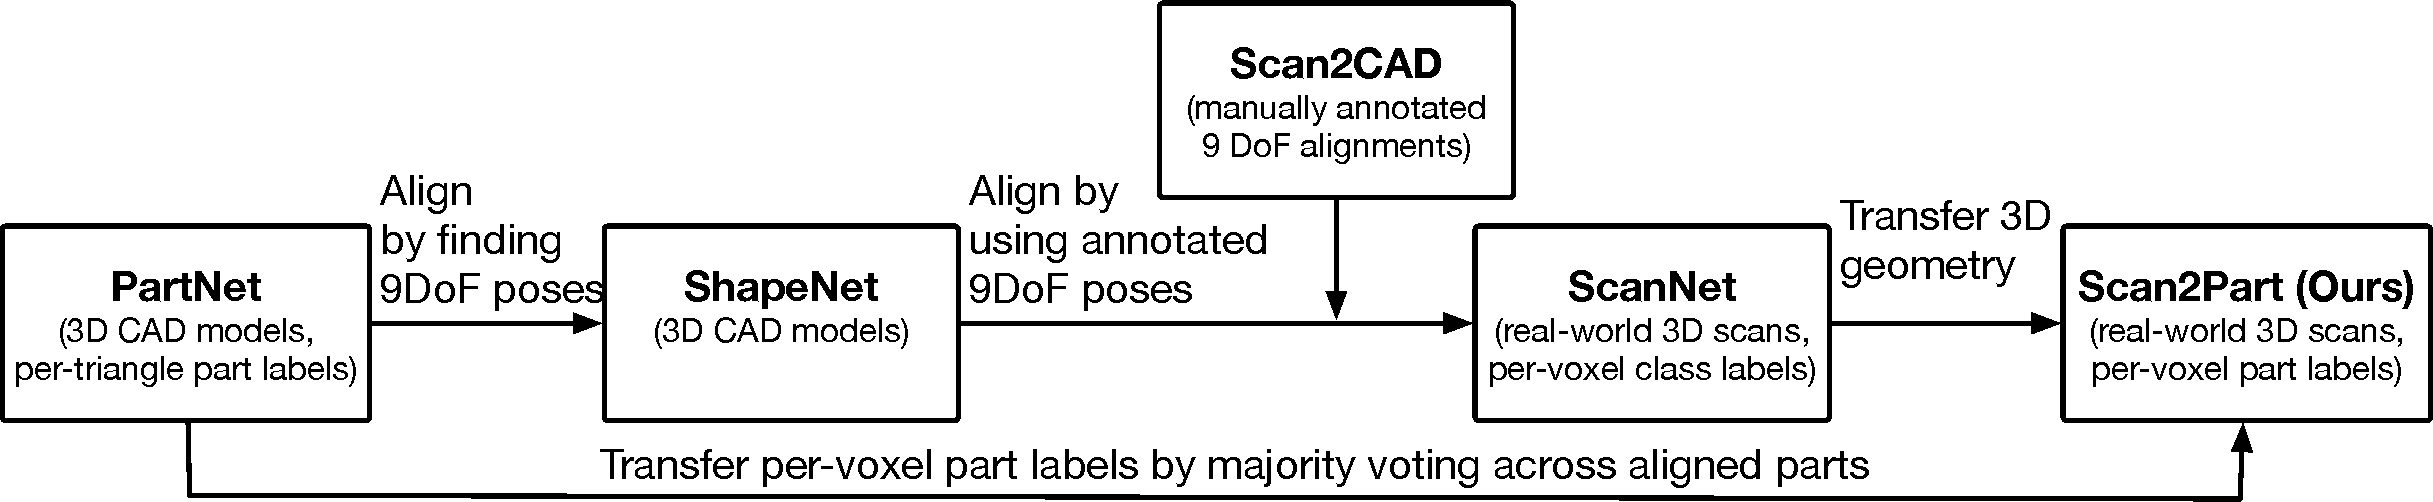
\includegraphics[width=0.99\textwidth]{Figures/scan2part/scan2part_labels_transfer.pdf}
\caption{Our automatic pipeline for part-based 3D scan annotation (see surrounding text).}
\end{figure}


% For this procedure to operate, one needs to register a set of 3D shapes to scans.
% Our resulting Scan2Part dataset consists of

This procedure results in 242,081 correspondences represented as 9\,DoF transformations between 1,506 reconstructions of real-wold ScanNet scenes and 53,618 unique parts of 2,477 ShapeNet objects.
Parts of each object have a tree structure, similar to~\cite{mo2019partnet}.
Note that the majority-based voting implementation of annotation transfer results in some semantic parts labels not being represented in the 3D scan, ultimately affecting parts taxonomy, which we discuss below. 

% we could sample or somehow ensure that at least some representatives of all classes exist in the dataset
% however, we have chosen the simplest implementation in the form of the simple majority voting 
% this results in some classes being omitted due to the finite scan resolution
% in the end, this affects part hierarchy

\begin{figure}[!t]
\label{fig:dataset_schema}
\centering
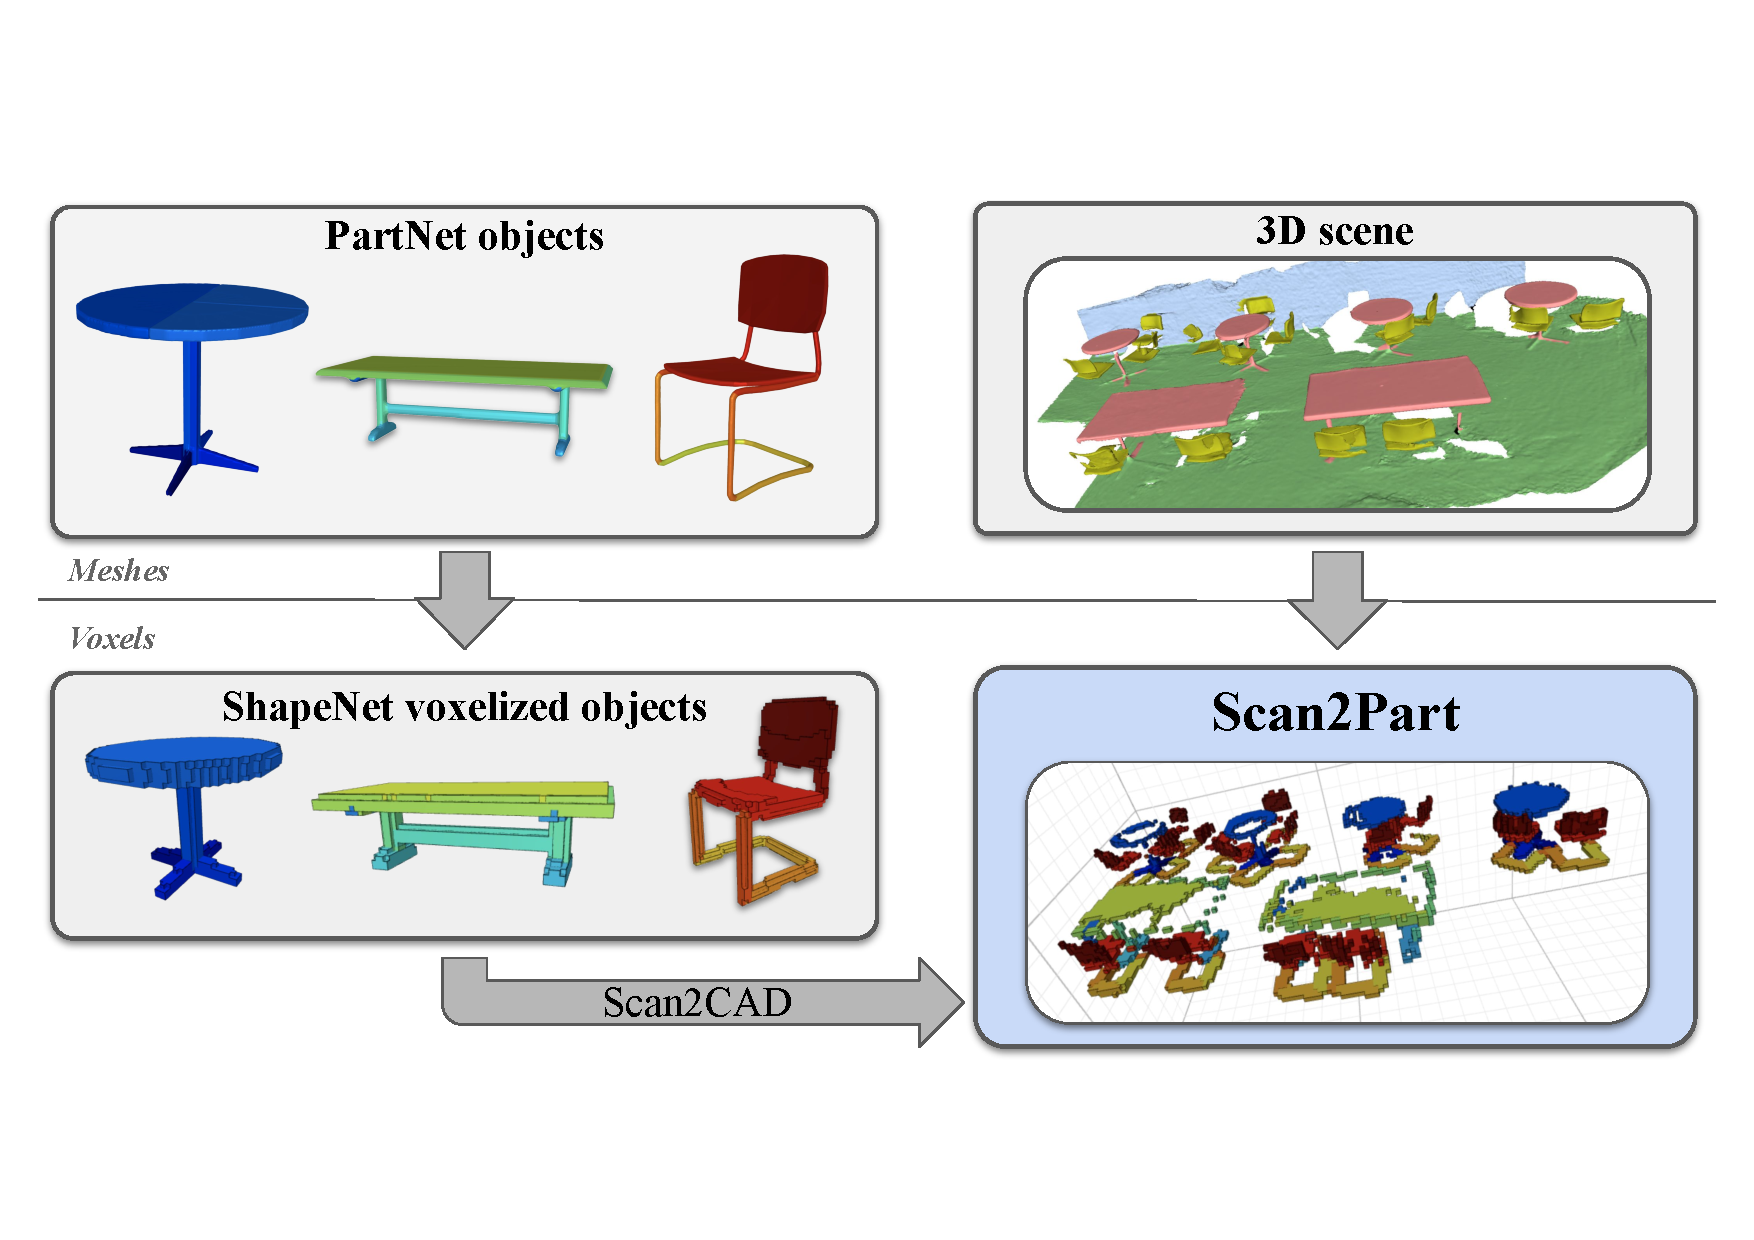
\includegraphics[width=0.9\textwidth]{Figures/scan2part/dataset_schema.pdf}
\caption{A pipeline for obtaining Scan2Part dataset. We project the PartNet \cite{mo2019partnet} labels to the ShapeNet \cite{chang2015shapenet} coordinate system (left), then use Scan2CAD \cite{avetisyan2019scan2cad} dataset to map labels to real scenes from Scannet \cite{dai2017scannet} (right).}
\end{figure}



% \begin{figure}[!t]
% \label{fig:part_level_variation}
% \centering
% 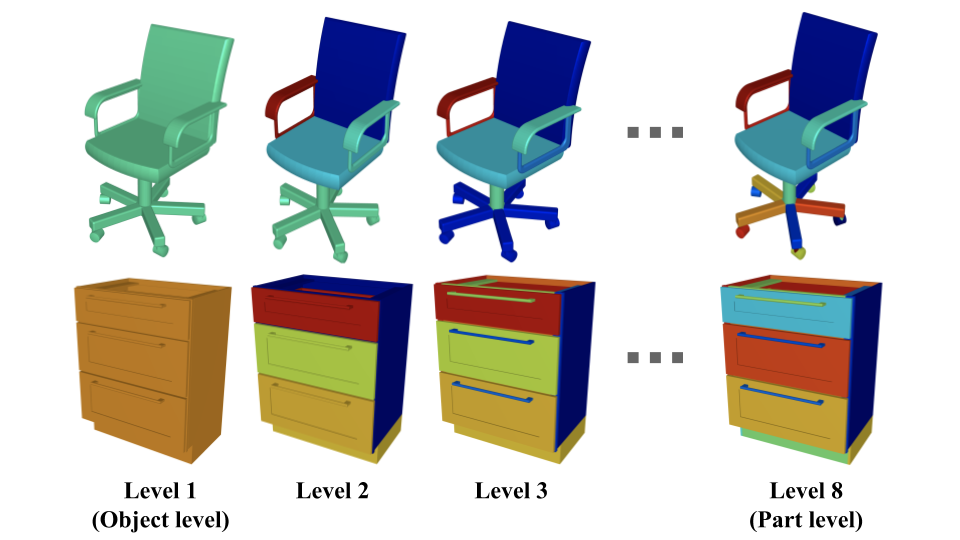
\includegraphics[width=\textwidth]{Figures/scan2part/part_level_variation.png}
% \caption{The object level of detail depending on the part taxonomy tree level based on PartNet taxonomy~\cite{mo2019partnet}. The level of detail  increases from left to right, starting with the object level.}
% \end{figure}

\paragraph{Parts taxonomy processing. } 
% % 1. description of the taxonomy
% % issue: classes that are not represented in 3D scans
% % 2. compressing taxonomy by merging classes
% % 3. compressing taxonomy by pruning the taxonomy tree
% % say something about taxonomy 
The taxonomy of 3D shape parts is represented as a single tree structure based on~\cite{mo2019partnet}. However, as the voxel resolution of the real-world 3D scan is relatively coarse, particular part categories (e.g., small shape details such as keyboard buttons or door handles) cannot be represented by sufficient number of 3D data points, thus implying a reduction in the original taxonomy. 
We proceed with this reduction by first choosing an appropriate occurrence threshold (we pick 1800 voxels, but demonstrate the effect of different threshold values in the supplementary) and remove classes that have smaller number of representatives in the dataset.
% % there are at least 1800 voxels labeled with this part\DZ{why 1800?}  in the entire dataset.
We finalize the taxonomy by pruning trivial paths in the tree (i.e., if a vertex has only one child, then we delete this vertex by connecting the child and the parent of this vertex), but keeping the leaf labels intact. We display the number of vertices at different granularities in the original and resulting part taxonomy levels in Table~\ref{tab:label_presence}.  
Some parts (leafs in the part taxonomy) are not represented in ScanNet data, so we remove these from the tree. 
% At the first tree level, each tree node  represents an entire object (bed, chair, table, etc.), at the second tree level --- the object base components (bed base, soft part, etc.), and so on.  An example of coloring an object by parts for different taxonomy levels is shown in the figure~\ref{fig:part_level_variation}
% %Each tree level is a level of object details: the deeper the tree level, the more detailed the parts division becomes.

% % we project partnet into scannet not vice-versa 
% % one could have done the other way around, e.g. say use subdivision (octrees) and place "ideal" CAD models into the scannet scenes, preserving ALL partnet classes 
% % but we're specifically interested in preserving as much as possible of the scannet noisy geometry 
% % additionally overlap between partnet and scannet categories is lower than 100%

% To build the part taxonomy, we choose the rules for combining the part trees of all the objects represented in Scan2Part. The total number of all instance parts is 242,081, while there are 53,618  unique parts (figure~\ref{fig:three_tables}, left).
% This is an extremely large number of labels for part segmentation, so we have to apply a more intelligent combination of part trees of different objects.
% If we assume that there are identical parts inside the same object, e.g., four table legs are four instances of the ``leg'' part (figure \ref{fig:three_tables}, center), then the total number of unique parts is reduced to 14,782. It is worth noting that in this case, the legs of different tables will be represented as different parts.

% However, if we assume that there are identical parts inside the same object class, i.e. all the legs of all tables are instances of ``leg'' part (figure \ref{fig:three_tables}, right), then the number of unique parts is reduced to 307.  

% % \DZ{It is unclear from the above what the rules actually are. It says if we assume this, then .., and if we assume that, then ...  Please state what exactly the rules are, and then explain why, e.g., to reduce the number of classes (and why this is a good thing)}

% Some parts (leafs in the part taxonomy) are not represented in ScanNet data, so we remove these from the tree. 
% A particular part is considered sufficiently represented if amount of voxels in the entire dataset labeled with this part is above certain threshold. 
% Through analysis of labels distribution we chose our threshold to be equal to 1800 voxels, but demonstrate the effect of different threshold values in the supplementary.
% % there are at least 1800 voxels labeled with this part\DZ{why 1800?}  in the entire dataset.
% After cleaning the tree, we get rid of trivial paths in the tree (if a vertex has only one child, then delete this vertex by connecting the child and the parent of this vertex) \DZ{what happens to labels?}  The number of vertices at different part taxonomy levels is shown in the table \ref{tab:label_presence}. 
% (\textcolor{red}{why do we use the first 3 levels?})

% \begin{figure}[!t]
% \label{fig:three_tables}
% \centering
% 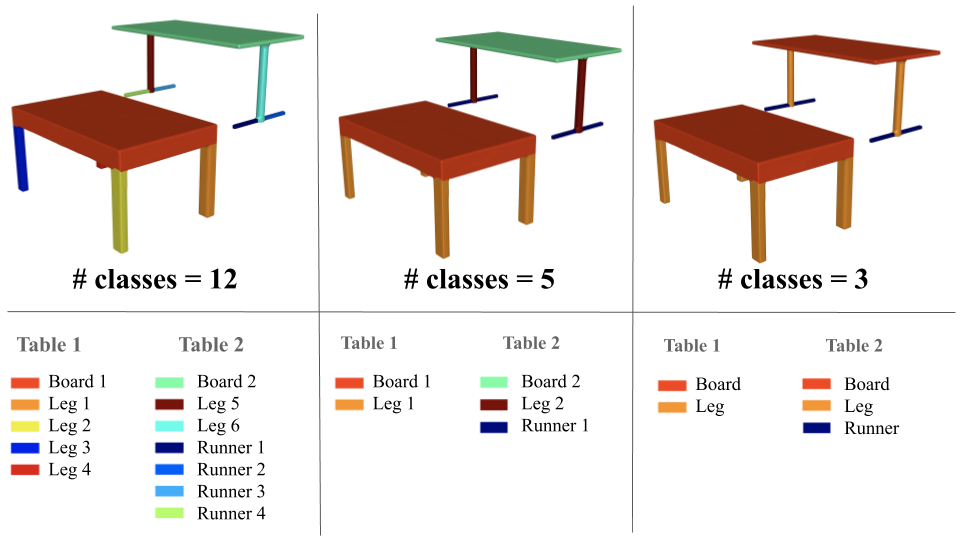
\includegraphics[width=0.9\textwidth]{Figures/scan2part/three_tables}
% \caption{Different rules for combining the part trees of all the objects. \textcolor{red}{TODO}: more specific. (left) if colors of all the legs are different, (center) if color of legs depends on the the table, (right) if color of all legs are the same.}
% \end{figure}


% \begin{figure}[!t]
% \label{fig:three_tables}
% \centering
% 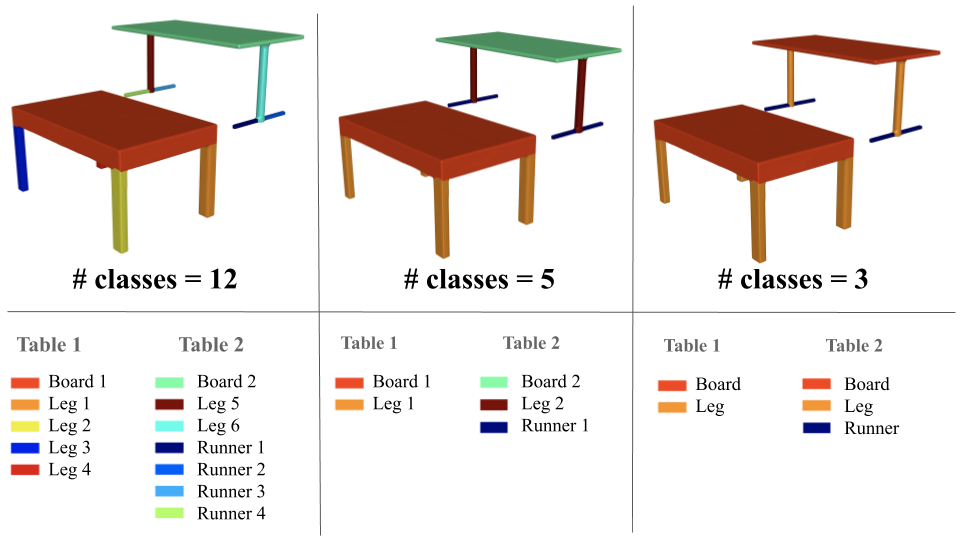
\includegraphics[width=0.9\textwidth]{Figures/scan2part/three_tables}
% \caption{Different rules for combining the part trees of all the objects. \textcolor{red}{TODO}: more specific. (left) if colors of all the legs are different, (center) if color of legs depends on the the table, (right) if color of all legs are the same.}
% \end{figure}





\begin{table}[ht!]
\centering
\caption{Number of parts on each tree level.
% \textcolor{blue}{@alex\_notch please double-check. numbers should be consistent over all the text}
}
\label{tab:label_presence}
\resizebox{0.8\textwidth}{!}{%
\begin{tabular}{l cccccccc}
\toprule
\multirow{2}{*}{\textbf{Level}} & \textbf{1} & \textbf{2} & \textbf{3} & \textbf{4} & \textbf{5} & \textbf{6} & \textbf{7} & \textbf{8} \\
& \textbf{(object)} & & & & & & & \textbf{(part)} \\
\midrule
Full Taxonomy & 18 & 50 & 133 & 223 & 269 & 302 & 306 & 307 \\
Sufficient Taxonomy & 13 & 36 & 79 & --- & --- & --- & --- & --- \\
\bottomrule
\end{tabular}
}
\end{table}


% In the last 4 years the field of computer vision saw an increase in Real-world 3D Scenes datasets acquired using depth sensors and LIDAR's, also level of detalization of object labels have increased, with complete object-part composition tree being the latest achievement~\cite{mo2019partnet}. The object part annotations were applied to meshes of objects that were created digitally and not measured by sensors. To address the problem of detecting object parts in real-world scans we needed a new dataset, so we decided to compose one ourselves from from four different sources.


% \begin{figure}
% \label{fig:dataset_overlap}
%   \centering
% 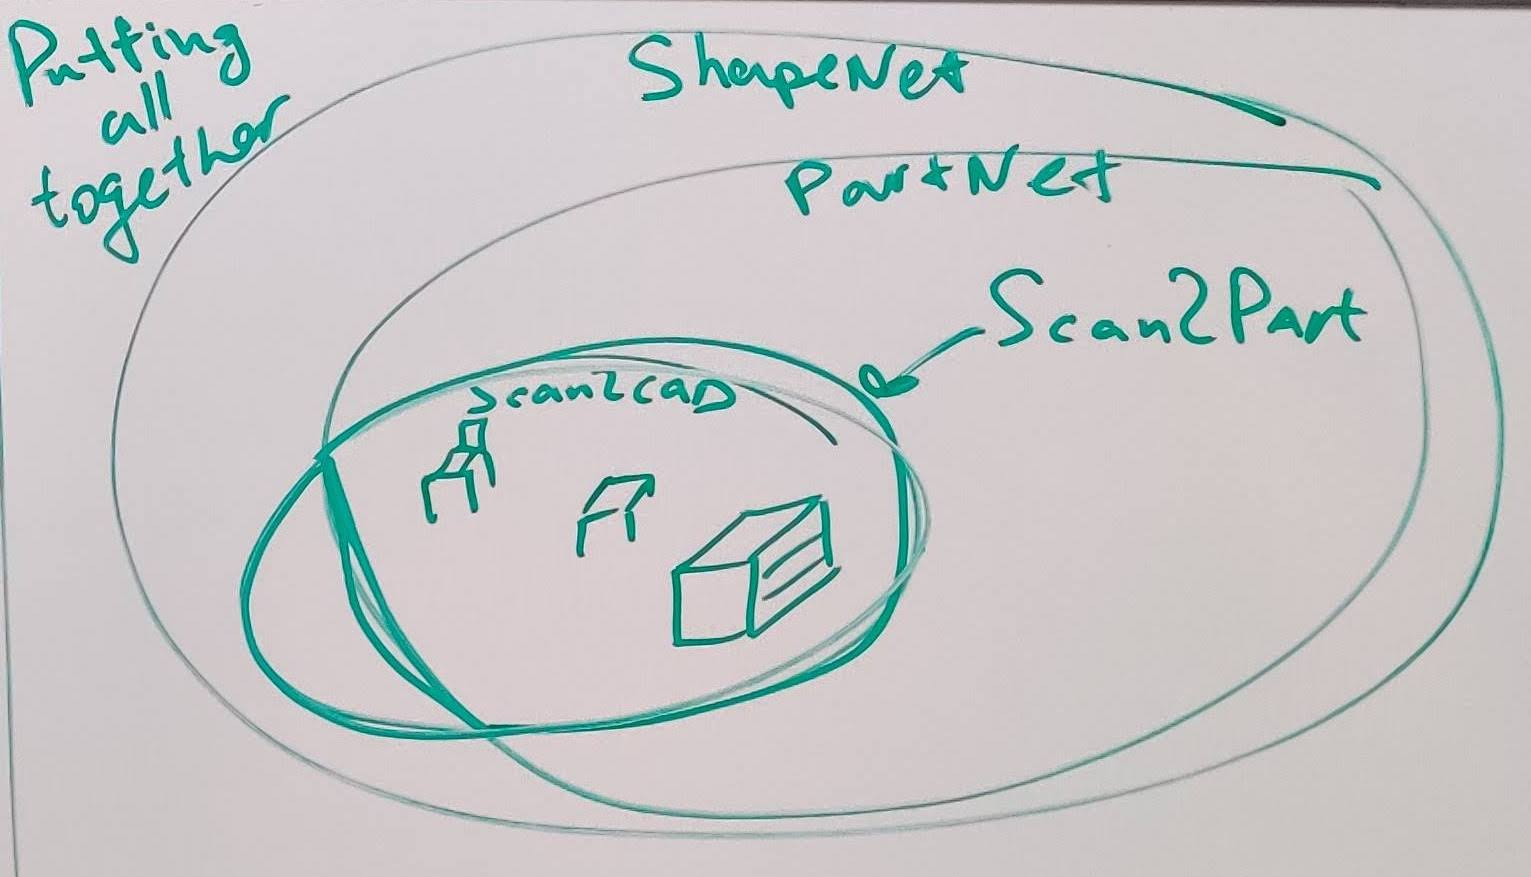
\includegraphics[trim=0 0 0 0, max width=0.5\textwidth]{Figures/scan2part/dataset_overlap.jpg}
% \caption{Venn Diagram of Datasets (PartNet $\subset$ Shapenet, Scan2CAD $\subset$  Shapenet)}
% \end{figure}

% \subsection{Labeling}
% \subsubsection{Shapenet to PartNet}
% \textbf{Projection}
% % \caption{left picture: gray shapenet, right picture: colored partnet}
% \textbf{ICP} 
% % \caption{two histogram of AVG CD between two objects: before and after ICP}
% % \caption{best and worst cases according to previous histogram}
% \subsubsection{Scan2CAD: ScanNet to Shapenet}
% % \caption{example from the Scan2CAD dataset}
% \subsection{Data-driven part taxonomy}

% After joining instance labels to class labels number of elements is reduced first to 53k, then to 20k, and finally to 308 classes.

% After further pruning because 20 of the part classes don't have a single voxel, number of classes can be reduced from 308 to 288 classes.
% % \caption{histogram of voxel appearance on the scenes}
% % \caption{example of prunned classes}
% % \caption{example of good class (not so deep)}
% \subsection{Model-driven part taxonomy}

% \subsection{Scan2Part}
% % \caption{tiser}

% \begin{table}[]
% \centering
% \caption{Dataset funnels}
% \label{tab:dataset_funnels}
% \begin{tabular}{l|l|l|l|l}
%  & Total count & PartNet & Scan2CAD & Scan2Part \\
% \hline
% Scenes from ScanNet & 1.5k & - & 1.5k & 1.5k \\
% Shapes from ShapeNet & 30k & 24k & 3k & 2.7k
% \end{tabular}
% \end{table}

% \begin{figure}
% \label{fig:Partnet_overview}
%   \centering
% % 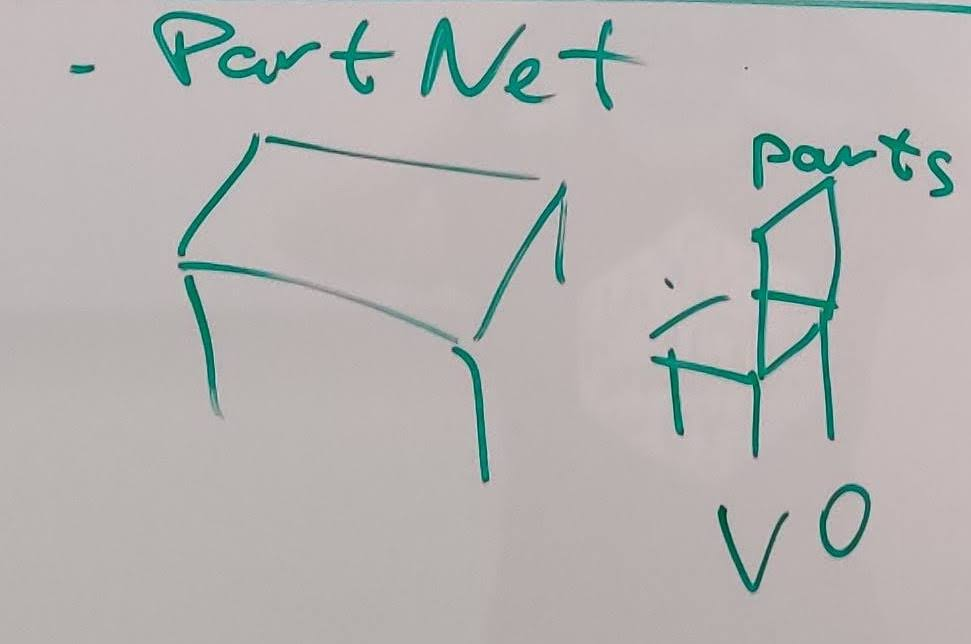
\includegraphics[trim=0 0 0 0, max width=0.5\textwidth, right]{Figures/scan2part/Partnet_overview.jpg}
% 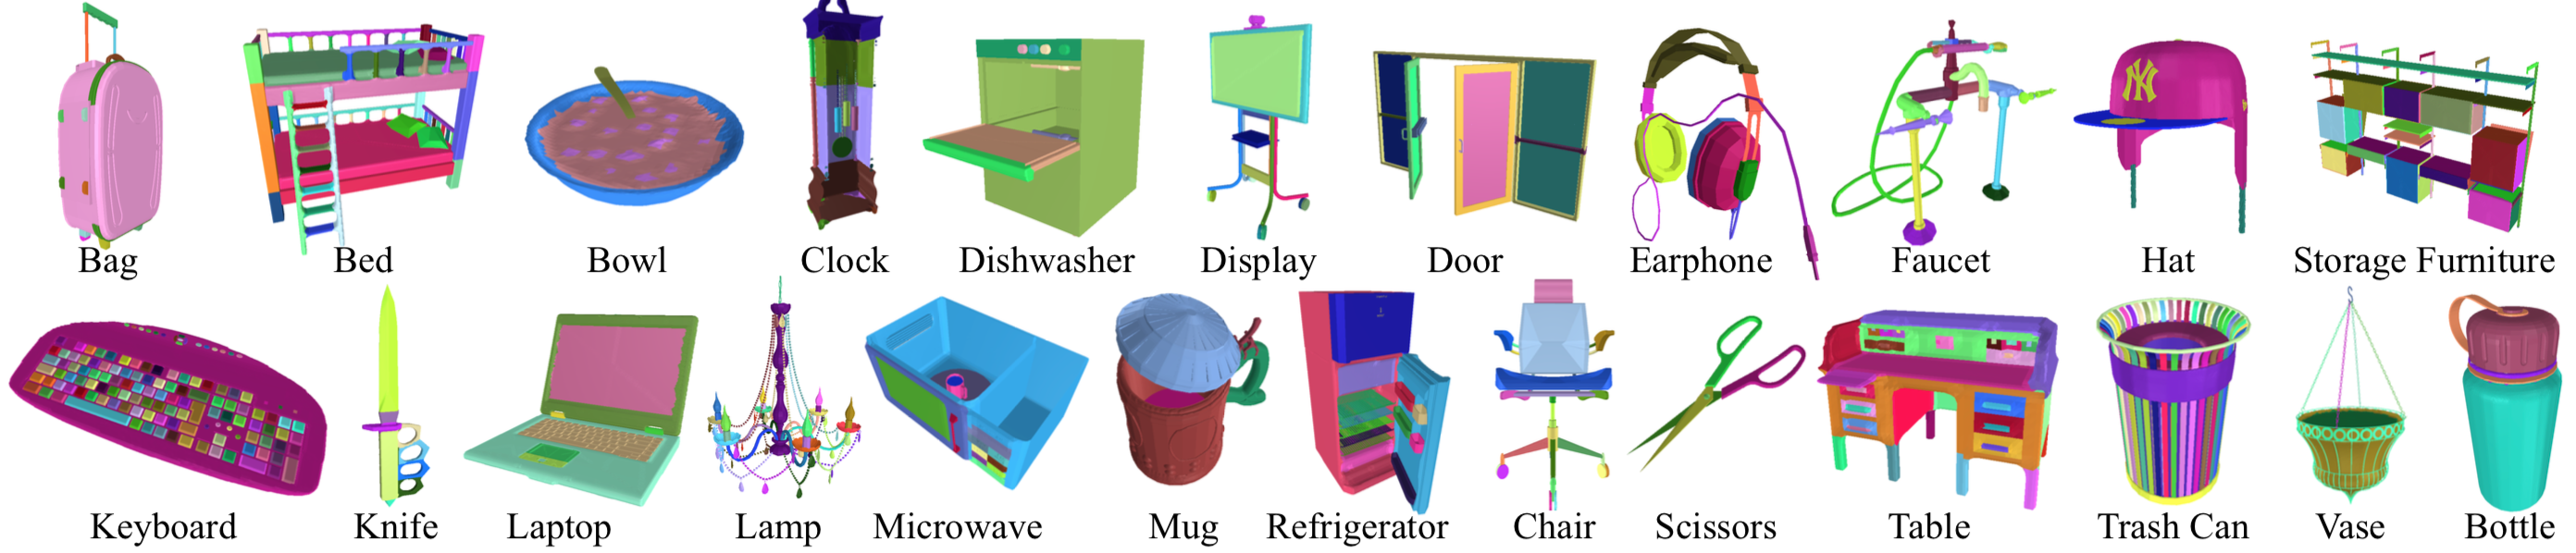
\includegraphics[trim=0 0 0 0, max width=\textwidth, right]{Scan2Part/images/partnet_data_visu.png}
% \caption{Partnet overview}
% \end{figure}

% В изображении~\ref{fig:partnet_to_scannet_labeling}а можно увидеть различие в детальности полигональной сетки в объектах датасетов ShapeNet и PartNet, высокая полигональность - последствие метода разметки деталей объекта в web-интерфейсе.
% На графике~\ref{fig:partnet_to_scannet_labeling}б изображено расспределение метрики Чамфера на соответствующих объектах в датасетах ShapeNet и PartNet, как можно заметить многие формы объектов в своих исходных положениях отличаются значительно. Поэтому для установления общей системы координат требуется решить задачу регистрации, которую мы решаем с помощью метода ICP~\cite{besl1992method}. На графике~\ref{fig:partnet_to_scannet_labeling}в можно увидеть как изменилось расспределние метрики Чамфера, ее высокое значение в некоторых случаях объясняется как нахождение методом ICP локального минимум соответствующему одному из симметричных положений объекта в разных датасетах, и не должно значительно повлиять на перенос разметки в датасет ShapeNet.  

% \clearpage

% % \begin{wrapfigure}{l}{0.25\textwidth}


% \begin{figure}[!htb]
% \label{fig:taxonomy_overview}
% \centering
% 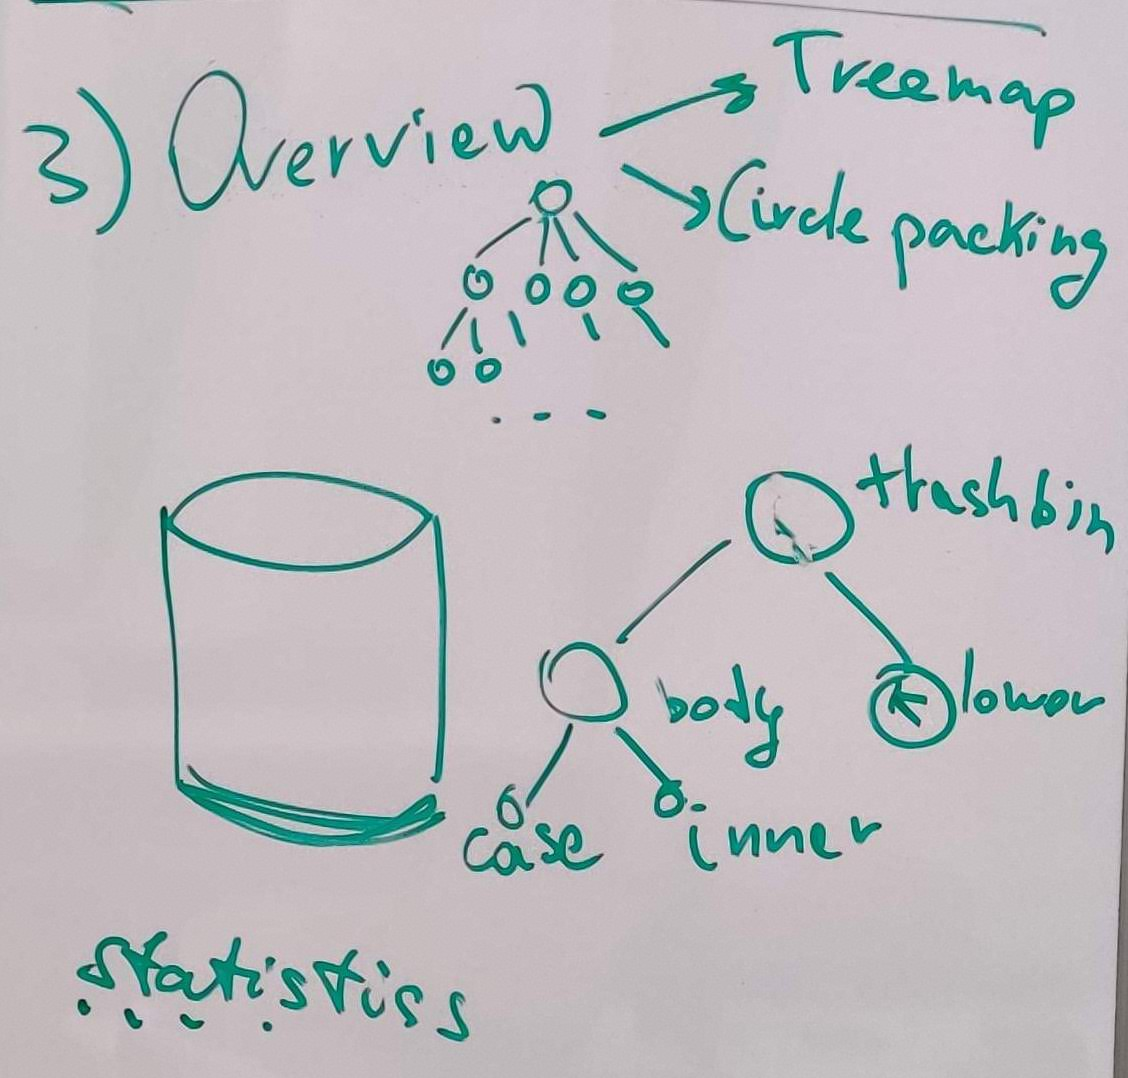
\includegraphics[trim=0 0 0 0, max width=0.5\textwidth]{Figures/scan2part/taxonomy_overview.jpg}
% \caption{taxonomy overview}
% \end{figure}


% \begin{figure}[!htb]
% \label{fig:scan2part_overview}
%   \centering
% 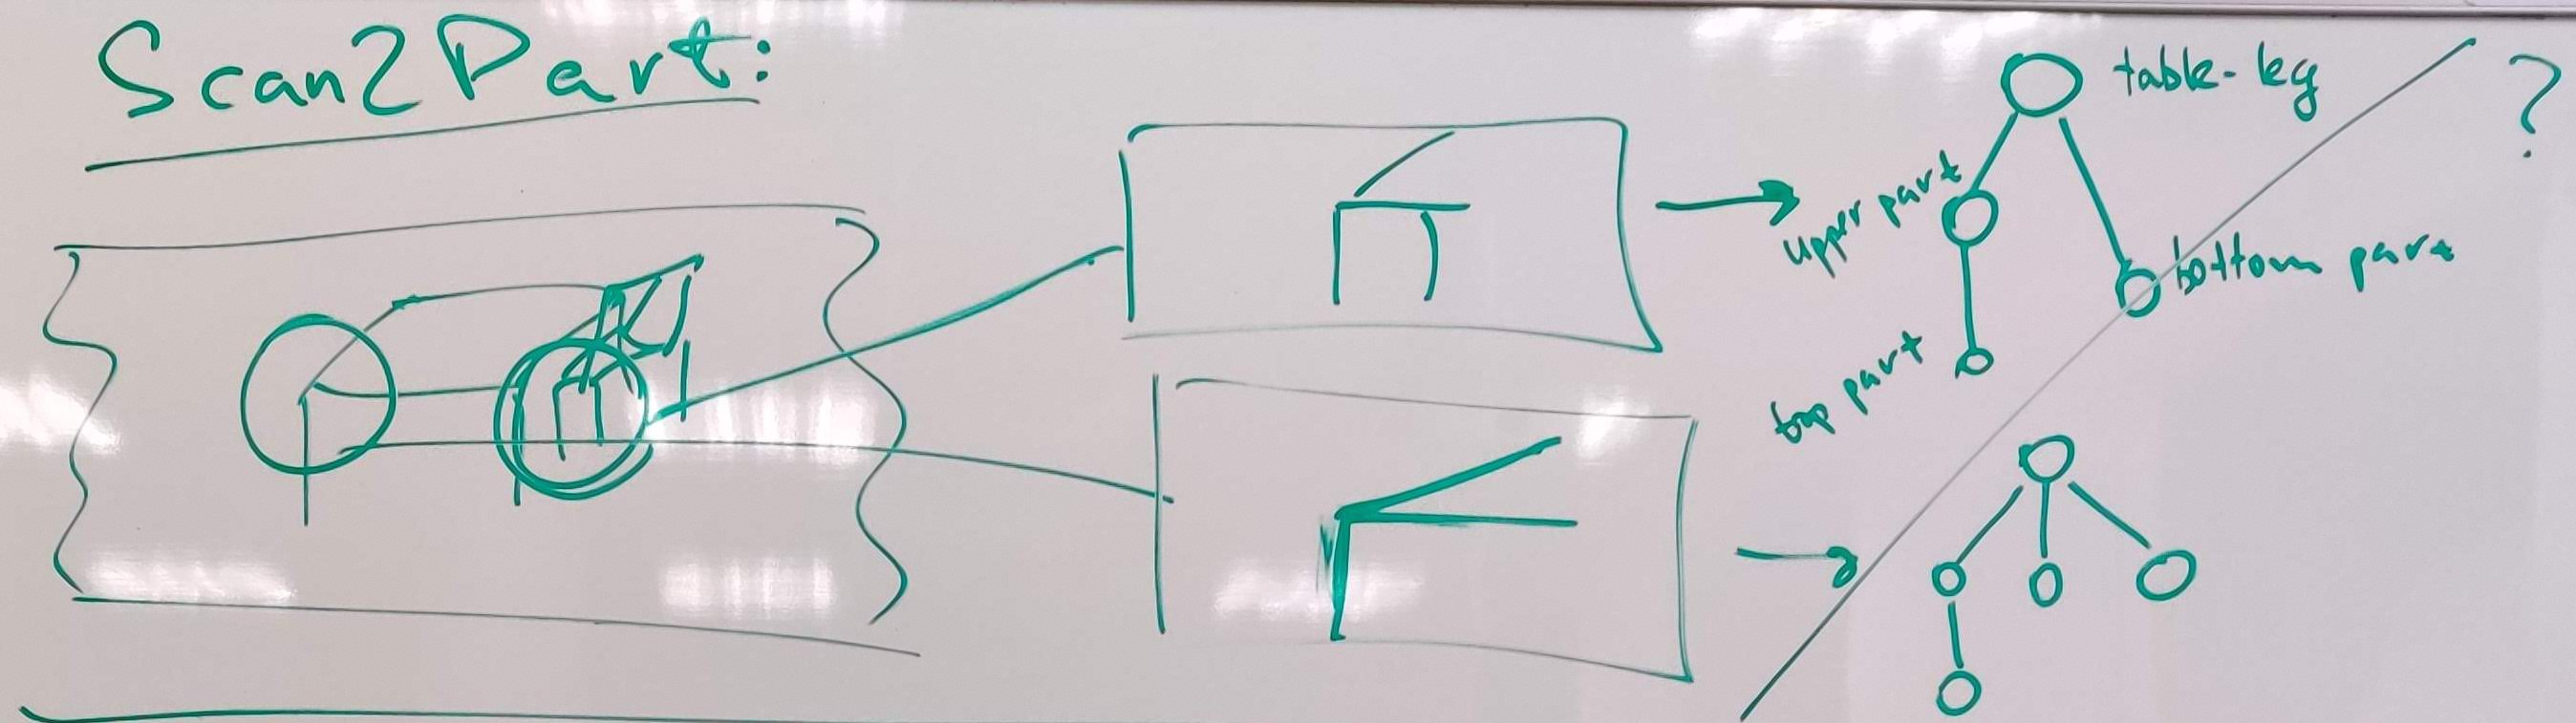
\includegraphics[trim=0 0 0 0, max width=0.5\textwidth]{Figures/scan2part/scan2part_overview.jpg}
% \caption{scan2part overview}
% \end{figure}
% \begin{figure}
% \label{fig:taxonomy_compression}
%   \centering
% 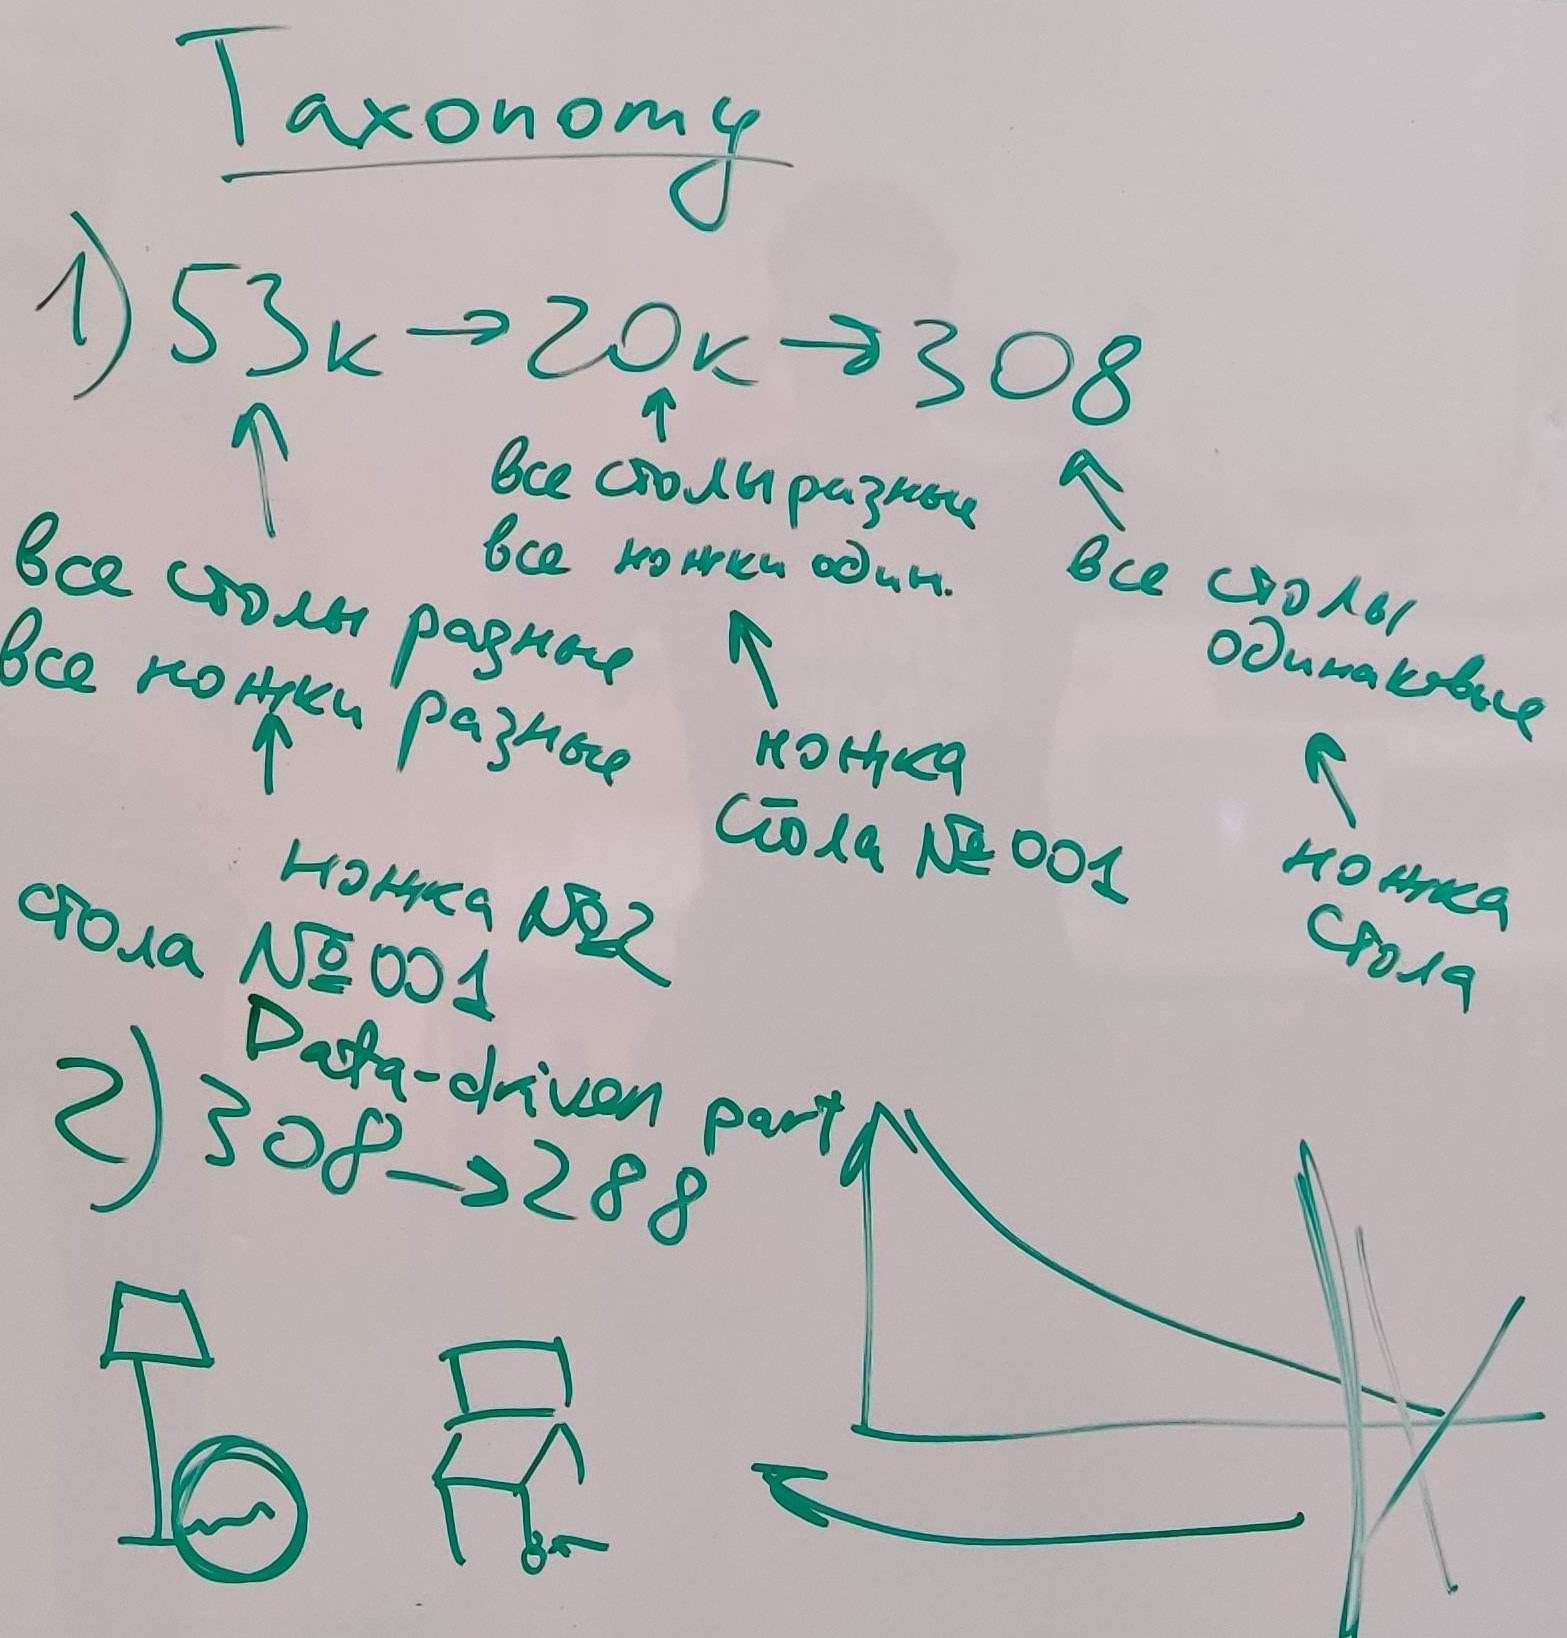
\includegraphics[trim=0 0 0 0, max width=0.5\textwidth]{Figures/scan2part/taxonomy_compression.jpg}
% \caption{taxonomy compression}
% \end{figure}

% \begin{figure}[!htb]
% \label{fig:dataset_mapping}
%   \centering
% 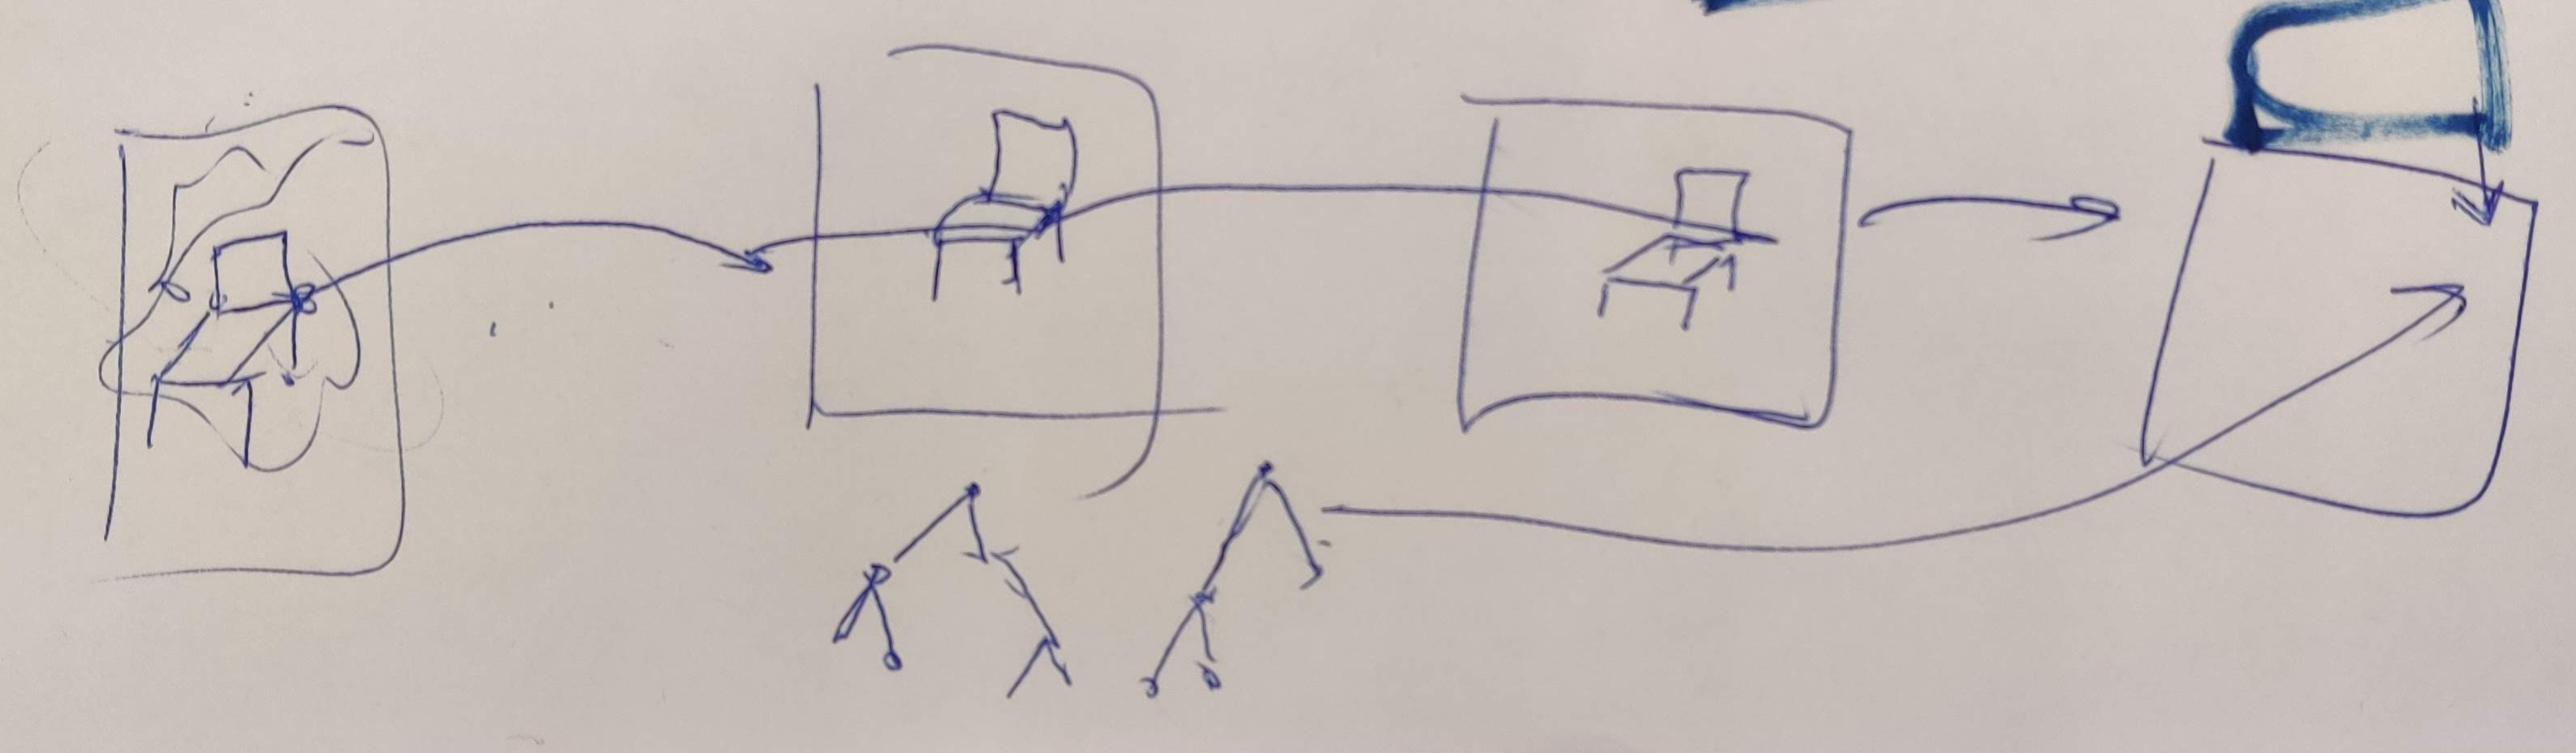
\includegraphics[trim=0 0 0 0, max width=\textwidth]{Figures/scan2part/dataset_mapping.png}
% \caption{Mapping of voxels in ScanNet scene to CAD model and to part hierarchy of the object}
% \end{figure}


% % \subsection{Scan2Part dataset preparation}
% The ScanNet \cite{dai2017scannet} is a dataset of RGB-D scans of real-world indoor scenes with multiple kinds of data representation and semantic object-level labels for those scans.
% The Scan2CAD \cite{avetisyan2019scan2cad} is a dataset that alignes CAD objects from ShapeNet \cite{chang2015shapenet} database to scenes from Scannet, therefore serving as a connective tissue to labels.
% The PartNet \cite{mo2019partnet} is a hierarchical instance level parts dataset of labeles for subset of ShapeNet database. The PartNet dataset the only dataset that has deep hierarchical structure compared to other part annotation datasets like in \cite{Yi16}.

% Using marching cubes algorithm we obtained a voxelised version of scenes from ScanNet dataset with object type labels and mapping of coordinate systems from ScanNet to ShapeNet, because of that we can calculate position of CAD object parts in the scene coordinate system and calculate relative volume in specific voxels thus projecting part labels on scene. 
% Under closer examination we discovered that most of the parts don't have a unique shape making task of instance segmentation for parts very hard to solve and not necessary for practical scene segmentation task.





% 
% 4) При решении собственно задачи понимания сцены на уровней частей естественно возникает некоторая иерархическая структура разметки. 
% — Выбор таксономии играет решащую роль при сегментации, так как слишком грубые таксономии будут неотличимы от просто сегментации и потому бесполезны, а слишком детальные не реализуются из-за ограничений разрешения и шума. 

% \begin{figure}[!t]
% \label{fig:dataset_teaser}
% \centering
% 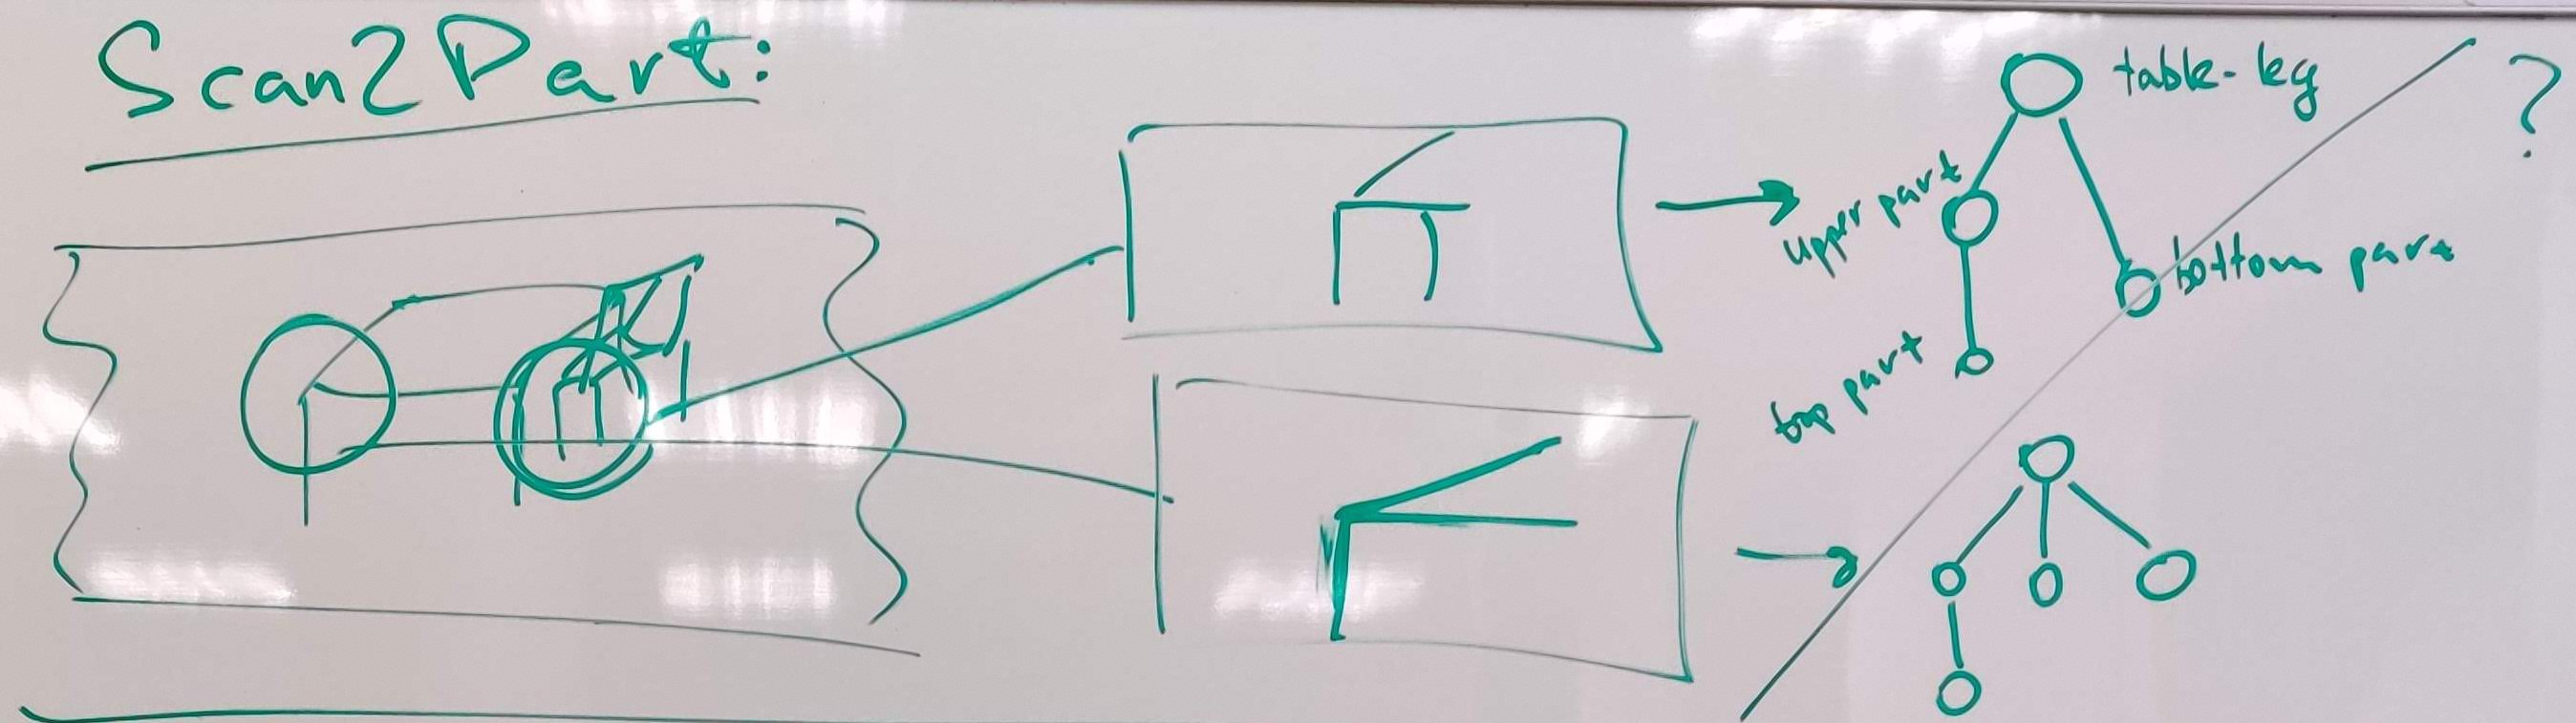
\includegraphics[width=0.9\textwidth]{Figures/scan2part/scan2part_overview.jpg}
% \caption{Dataset teaser}
% \end{figure}

%


% \textcolor{red}{TODO}: Table with abovementioned numbers.



\section{Methodology}
\label{sec:methods}

\paragraph{Classes of 3D understanding tasks. }
\label{methods:tasks}
We consider three distinct classes of challenging part-level 3D scene understanding tasks: semantic labeling, hierarchical semantic segmentation, and instance segmentation. 
The input to all our models is the voxelized scene SDF, representing 3D geometry without associated RGB values.

In~\emph{semantic labeling,} the goal is to associate a set of $n$ semantic part labels~$y_j = (y_j^{d_1}, \ldots, y_j^{d_n})$ with each voxel~$v_j$, 
at detail levels~$d_1, \ldots, d_n$.
To predict parts in such multi-label formulation, we produce a set of softmax scores $p_j = (p_j^{d_1}, \ldots, p_j^{d_n})$.
We train the network in multiple setups, differing by the structure of supervision available to the network, each time evaluating labeling performance at each detail level $d_i$. Specifically, we define 
our loss function $L$ to be a weighted sum of cross entropy losses for each level of detail
\begin{equation}
\label{eq:semseg_loss}
L(p, y) = \sum_{k = 1}^K \alpha_k L_{\text{CE}}(p^k, y^k)
\end{equation}
and specify a set of weighting schemes for $\alpha_1, \ldots, \alpha_K$. 
This loss structure allows expressing both ``flat'' segmentation formulations (e.g., choosing $\alpha_{k} = \delta_{ki}$ to segment at level $d_i$ only), that we view as baselines, and multi-task formulations that integrate training signal across multiple levels of semantic detail.

For this task we 

To perform \emph{hierarchical semantic segmentation,} one must perform segmentation at multiple levels in the hierarchy, inferring labels in coarse- and fine-grained detail levels simultaneously. 
Similarily to~\cite{mo2019partnet}, we approach this task using \emph{bottom-up,} \emph{top-down} and \emph{ensemble} method.
Bottom-up method performs segmentation at the most fine-grained level and propagates the labels to object level, leveraging the taxonomy structure.
Conversely, the top-down approach infers labels first at coarse level (starting with objects) and subsequently at finer levels (parts), recursively descending along predicted taxonomy branches.
With the ensemble method, predictions of networks independently trained at distinct detail levels are integrated in a joint inference step.
We note that \emph{multi-task training} using~\eqref{eq:semseg_loss} also results in a hierarchical segmentation method, and include it in the comparison.






% we use a set of linear layers and project voxel features to labels, producing

% The model assigns the input  to several classes \DZ{unclear -- one of several classes?  what is depending on what?}  depending on the total number of part classes on the selected level of detail (LoD) of objects part taxonomy.
% The distribution of class labels on all of LoDs is very unbalanced, as shown on the treemap diagram \ref{fig:class_distribution_treemap}.
% On a given level of detail $k$, the frequency of  a voxel class $i=0 \ldots N^k$ is denoted $C_i^k$.  Then the Cross Entropy loss function weights for class $i$ are equal to $w_i^k = \frac{\max_{i=0 \ldots N^k} (C_i)}{C_i}$.
% If the model is trained to predict labels for several levels of detail $\{k,n,p\}$ we use multiple linear layers to project each voxel features to labels. The final loss function $L$ is computed as a weighted sum of Cross Entropy losses for each level of detail: 
% \[L = \sum_{j\in\{k,n,p\}} w_j L_j
% \]

% flat softmax at lod=1,2,3, and multiloss(12, 123), with quality computed separately (+bottom up deduced labels), +topdown with own softmax labels with masking all of the other labels: here inference would be, choose heads which are predicted as positive, and go one level down inferring, ensemble 


% — В этой работе в качестве отправной точки мы выбрали реализацию двух подходов, topdown и bottomup, в качестве двух основных стратегий интеграции разметки на различных уровнях детализации. 
% — Кроме того, мы исследуем различные схемы взвешивания сигналов на разных уровнях таксономии, неявно кодирующие редукцию таксономии.

% Overall, semantic and hierarchical segmentation tasks have been considered in multiple settings:
% \begin{enumerate}
% \item Bottom-up approach: Segmentation of part labels on different levels of detalization from object level to 3 levels of hierarchy down
% %\textcolor{blue}{VI: Первое упонимание о трех уровнях иерархии частей, хотя на данном этапе нет ни одного упонимания датасета. Вероятно, лучше описание датасета поместить перед методологией (в Scan2CAD сначала идёт описание датасета).}
% , which, in turn, allows us to compute predictions for higher labels.% this approach sometimes called "Bottom-Up".

% \item Top-down approach:  each sub-part segmentation is performed in parallel in separate linear projections from voxel features (masked by ground truth of parent part labels).
% \DZ{why is this top-down?} \AN{In test-time predictions computed from root node of hierarchy and then depending on the predicted classes sub-part classified by the "head" dedicated to that node, it does that until terminal node (leaf) is reached.} \DZ{Ok I got the explanation above, but still do not understand the linear projection part; I leave it to AN or AA to rewrite}

% \item Ensemble Segmentation \cite{mo2019partnet}  on all levels at the same time, projecting the voxel features to 3 different heads and testing different weighting schemes to weigh all of the losses.
% \end{enumerate}



% Besides semantic segmentation, we also perform instance segmentation on level of objects and on the level of parts. 

For \emph{instance segmentation,} the goal is to simultaneously perform part-level semantic labeling and assign each voxel~$v_j$ a unique part instance ID (e.g., to differentiate separate legs of a table).
To this end, we employ a discriminative loss function which has demonstrated its effectiveness in previous works~\cite{de2017semantic,pham2019jsis3d}.
To efficiently train on our highly unbalanced data, we additionally enforce separation between objects and background representations in feature space (see supplementary for details).

Suppose that there are $K$ instances and $N_k, k\in\{1,...,K\}$ is the number of voxels corresponding to $k$-th instance, $\mathbf{e}_j \in \mathbb{R}^d$ is the embedding of voxel $v_j$, and $\boldsymbol\mu_k$ is the mean of embeddings for the $k$-th instance. The embedding loss $\mathcal{L}_{embedding}$ of a discriminative function can be defined as follows,

\begin{align}
  \label{eq:discriminative}
  \mathcal{L}_{embedding} = \alpha \cdot \mathcal{L}_{pull} + \beta \cdot \mathcal{L}_{push} + \gamma \cdot \mathcal{L}_{reg}
\end{align}
where
\begin{align}
  \label{eq:pull}
  \mathcal{L}_{pull} = \frac{1}{K} \sum_{k=1}^K \frac{1}{N_k} \sum_{j=1}^{N_k} \left [ \left \Vert \boldsymbol\mu_k - \mathbf{e}_j \right \Vert_2 - \delta_v \right ]^2_+
\end{align}
\begin{align}
  \label{eq:push}
  \mathcal{L}_{push} = \frac{1}{K(K-1)} \sum_{k=1}^K \sum_{m=1, m \neq k}^K \left [2\delta_d - \left \Vert \boldsymbol\mu_k - \boldsymbol\mu_m \right \Vert_2 \right ]^2_+
\end{align}
\begin{align}
  \label{eq:reg}
  \mathcal{L}_{reg} = \frac{1}{K} \sum_{k=1}^K \left \Vert \boldsymbol\mu_k \right \Vert_2
\end{align}
where $[x]_+=\max(0,x)$, $\delta_v$ and $\delta_d$ are respectively the margins for the pull loss $\mathcal{L}_{pull}$ and push loss $\mathcal{L}_{push}$. We set $\alpha = \beta = 1$ and $\gamma = 0.001$ the same way as in implementation we used as a reference~\cite{pham2019jsis3d}.

Embedding loss can be understood as follows: the pull loss $\mathcal{L}_{pull}$ pulls embeddings of voxels of some instance towards the centroids, $\boldsymbol\mu_k$, at the same time the push loss $\mathcal{L}_{push}$ pushes these centroids away from each other. The regularisation loss $\mathcal{L}_{reg}$  forces all centroids towards the origin. If we set the margin $\delta_d > 2\delta_v$, very useful property of this loss as described in paper~\cite{de2017semantic} will emerge, the ability to learn the voxel embeddings that will be closer to the instance centroid they belong to, rather than other centroids of other instances.

% \LA{either show the loss here, or refer to supplementary: (see supplementary for details)}
Compared to architectures that use region proposal modules~\cite{yi2019gspn,pham2019jsis3d,engelmann20203d}, this results in a more computationally lightweight architecture, while reducing instance segmentation problem to a metric learning task.
At inference time, we cluster voxel feature vectors to produce part instances in a scene using mean-shift algorithm~\cite{comaniciu2002mean}.

\paragraph{Network and training.}
\label{methods:network_training}
Our models for semantic and instance segmentation tasks are 3D CNNs identical in architecture up to the last layer. %, computing voxel features.  
Specifically, as a backbone for our models we use a 3D version of the U-net architecture~\cite{RFB15a} with residual modules in both encoder and decoder branches (based on~\cite{cciccek20163d,lee2017superhuman}; see supplementary for a full network architecture), including convolutions, ReLU, and group normalization layers.
 % has been shown to be efficient for many semantic segmentation tasks.
For each input voxel, the network produces a 32-dimensional feature vector that is further appropriately transformed by the last layer, accommodating a required number of predicted classes. All our networks are fully convolutional, enabling inference for scenes with arbitrary spatial extents.
% For this reason, we are going to use it as a backbone for our models, changing only last layer to 

% \VI{Why Unet? Is this a current SOTA? is 22-27\% close enough to what the current SOTA shows?}

% We use 4 residual modules in the encoder and 3 in the decoder parts of U-net architecture. 
% The number of channels in hidden layers of the encoder increases by 64 in each module and is equal to 256 at the network's bottleneck.
% In the decoder, the number of channels decreases by 64, with  32 channels in the last layer, giving us rich feature vectors for each voxel. 

%\textcolor{blue}{VI: Может нагляднее будет нарисовать Encoder-Decoder? Или представить параметры в виде таблички}

% \begin{figure}
% \label{fig:class_distribution_treemap}
%   \centering
% % 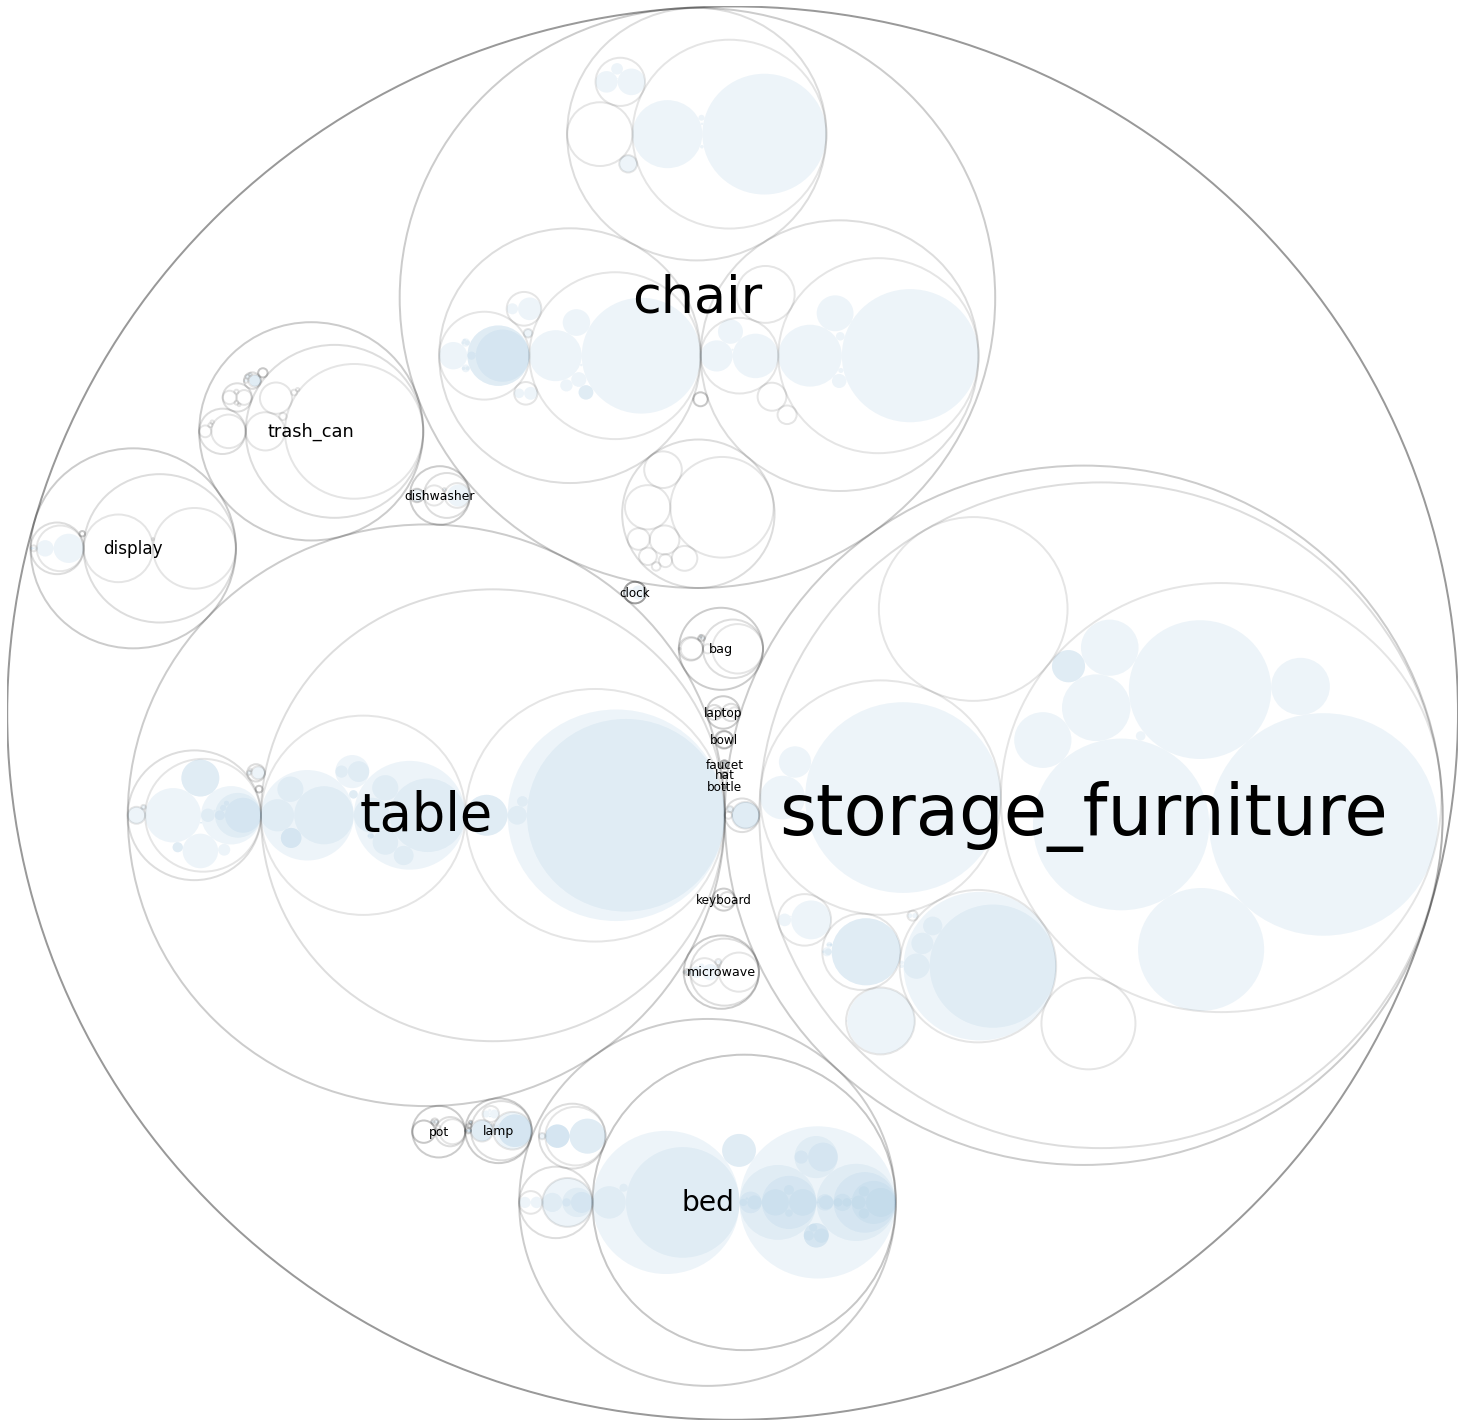
\includegraphics[trim=0 0 0 0, max width=\textwidth]{Figures/scan2part/treemap_v2.png}
% % trim=left bottom right top
% 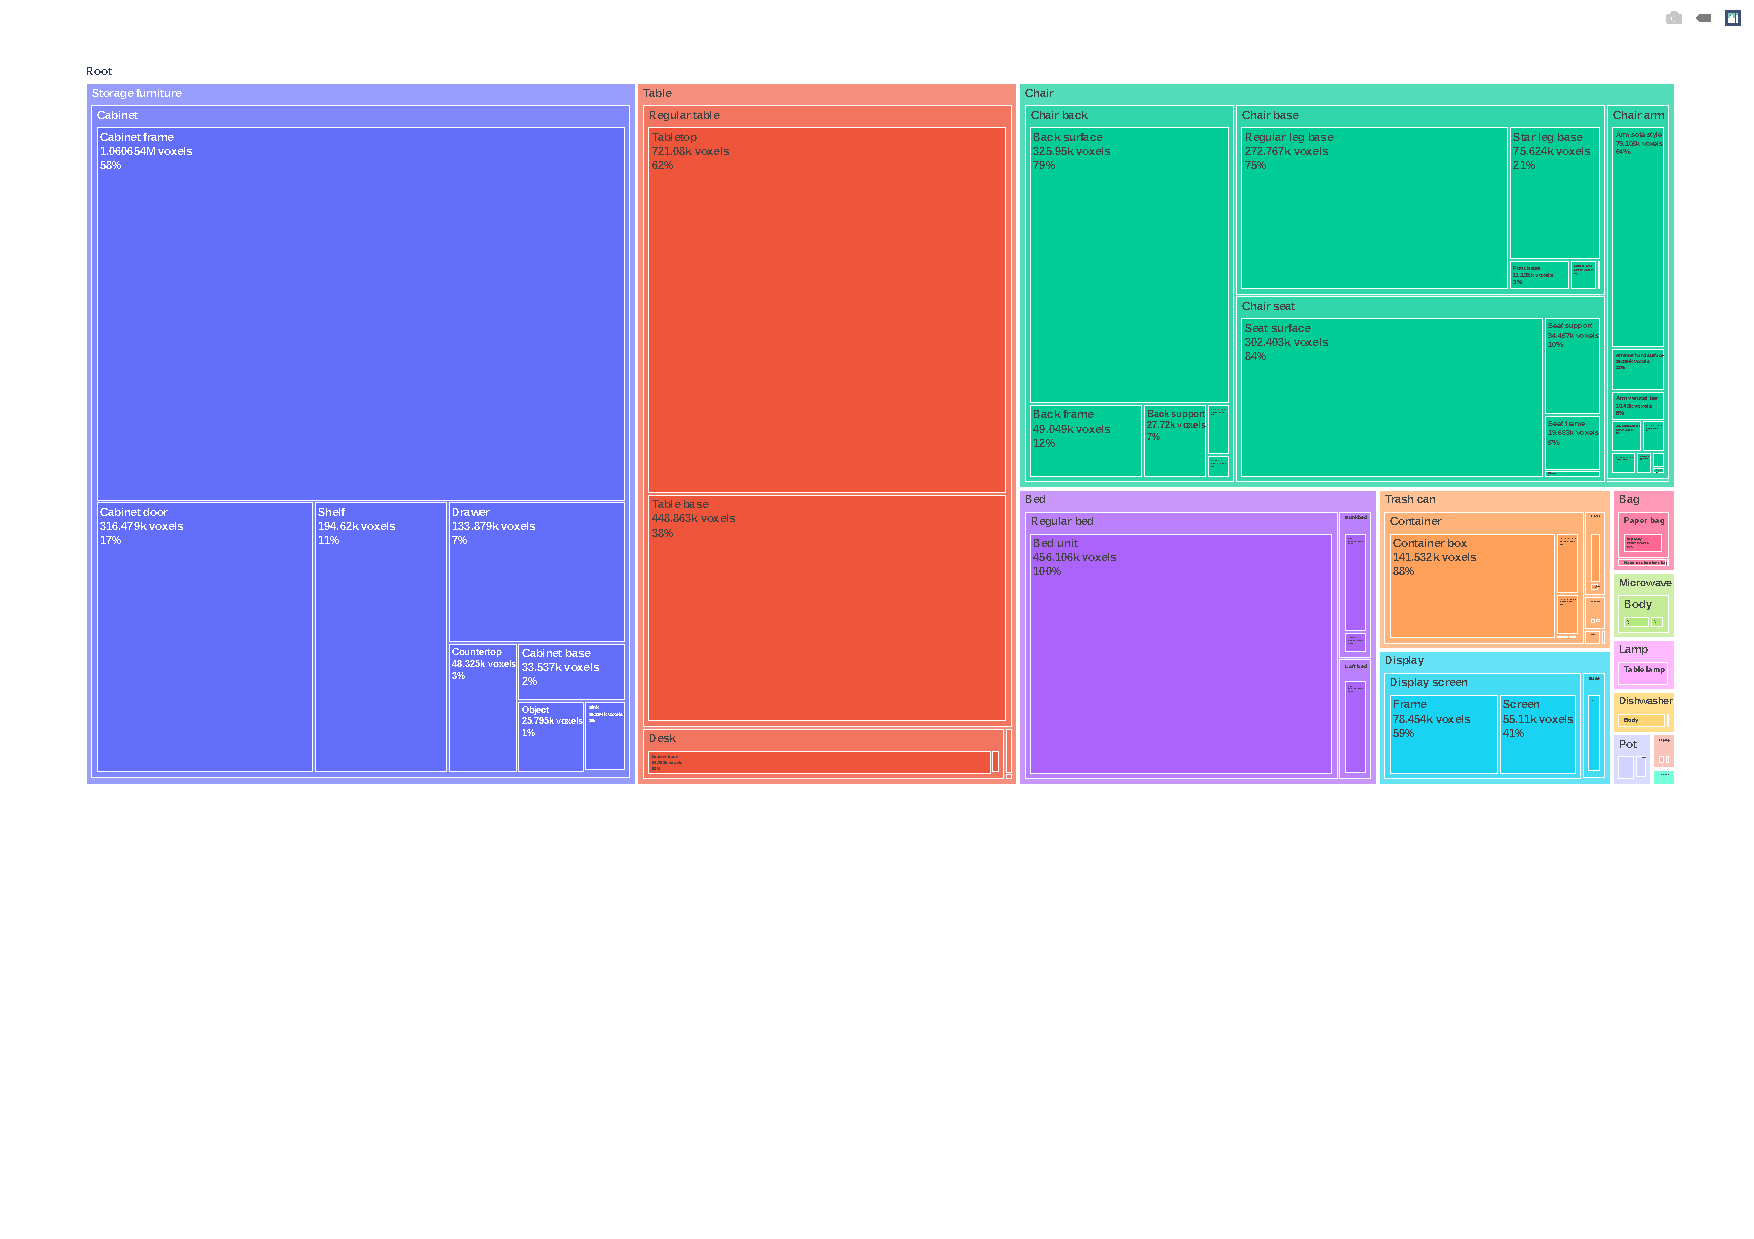
\includegraphics[trim=0 220 0 20, clip, max width=\textwidth]{Figures/scan2part/treemap_plot.pdf}
% \caption{Frequencies of classes in the part hierarchy. The areas of circles are proportional to the number of part voxels as a fraction of the number of voxels in the parent part.}
% \end{figure}


% \begin{figure}
% \label{fig:segmentation_architectures}
%   \centering
% 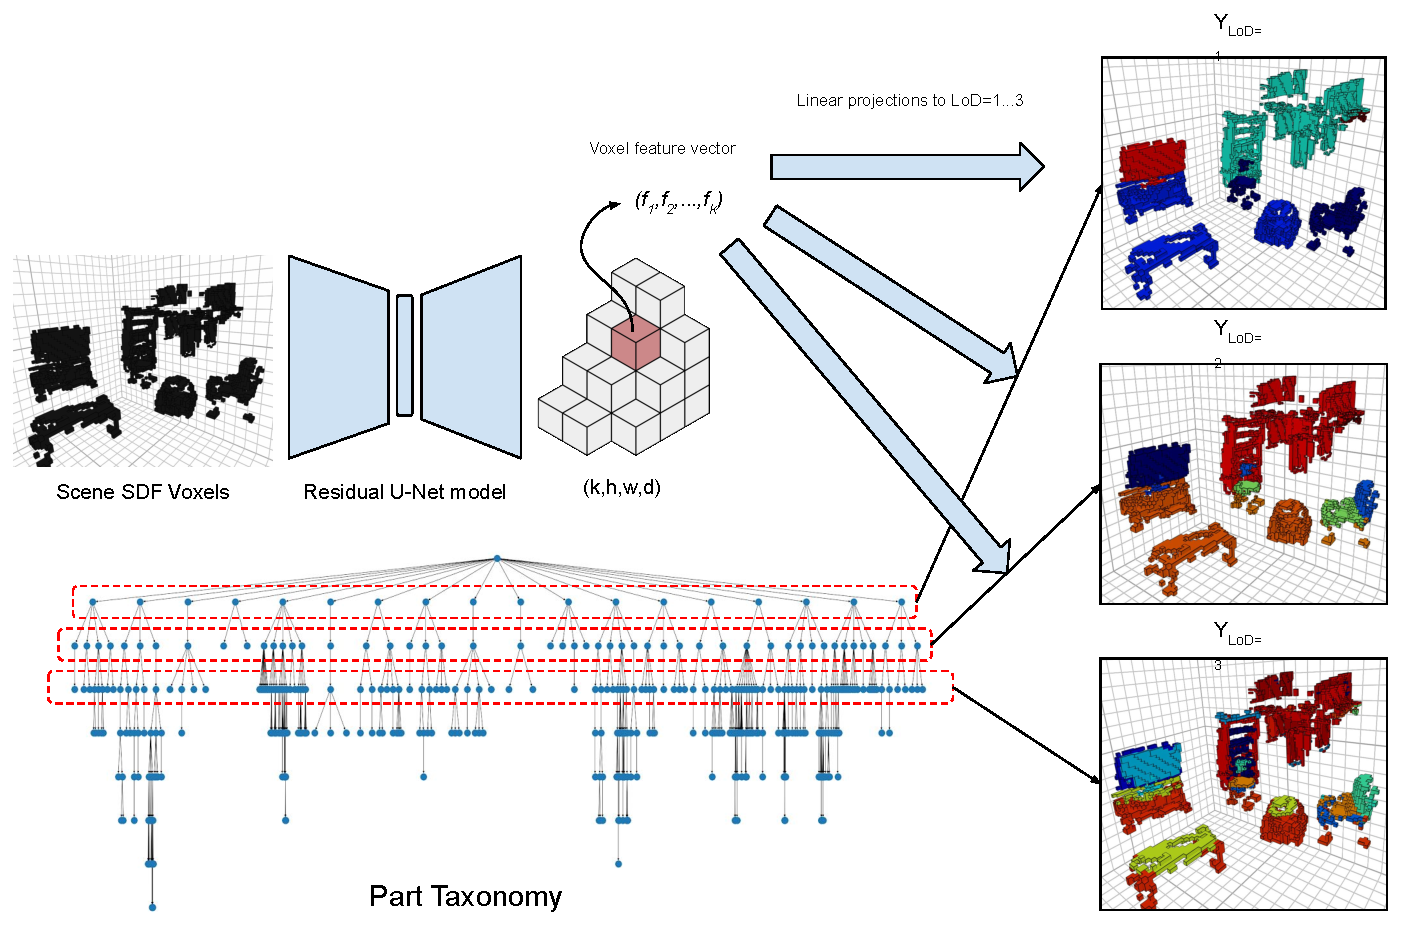
\includegraphics[trim=0 0 0 0, max width=\textwidth]{Figures/scan2part/architectures.pdf}
% \caption{Architectures of different segmentation models in different setups.}
% \end{figure}

% We compute a stratified train/test split, keeping split class ratios close to those in the whole dataset.
% Train and test sets were selected using combinatorial optimization routine that tries to split voxels of a class in ratios close to that of whole split.
We select 80\% of the scenes in ScanNet for training, keeping $1/16$ as a mini-validation to tune hyperparameters, and put aside 20\% scenes for testing.
During training, we extract 16~volumetric crops of size~$64^3$ from each voxelized scene and randomly shuffle them across all scenes in the training split.
% 16 crops were extracted from each scene, and shuffled with all other crops from other scenes.
The batch size we use ranges from 4 to 48 in different experiments, subject to fitting the network into the available GPU memory.
We optimize our models using Adam~\cite{kingma2014adam}, initalizing learning rate proportionally to the batch size, and decreasing it on pre-selected milestones by a factor $0.2$, with a weight decay of $10^{-4}$.
% for example for batch size = 32 base_lr=0.003, for bs=8 base_lr=0.001, for 48 base_lr=0.005 or 0.01 of it was too slow in training
We train until early stopping with patience parameter of 10, or until we reach a maximum epoch limit of 200.


% \DZ{unclear why different numbers where used}
% The encoder and the decoder consisted of 4 residual blocks each,  with output layers with  32 features for each voxel.
% Residual blocks included convolution, followed by ReLU non-linearity and group normalization with number of groups equal to 8.
% DZ already said this 
%Input tensors had only one channel the value of SDF function in that voxel.

\paragraph{Model configurations for different tasks}
\label{results:model_configs}
Table~\ref{table:configurations} summarizes our model specifications, differing by the choice of weights in~\eqref{eq:semseg_loss}.
To simplify the training process we assume all of the weights for loss functions to be normalized: $\sum_i \alpha_i = 1$.


\section{Experimental Results}
\label{sec:results}

\begin{wraptable}{r}{5.5cm}
\caption{Model configurations that we consider, with $\alpha_i$ in~\eqref{eq:semseg_loss}.}
\begin{tabular}{lrrr}\\\toprule  
Configuration   & $\alpha_1$ & $\alpha_2$ & $\alpha_3$ \\
\midrule
Base coarse     & 1 & 0 & 0 \\
Base middle     & 0 & 1 & 0 \\
Base fine       & 0 & 0 & 1 \\
MTT-12          & .5 & .5 &  0 \\
MTT-123-coarse  & .5 & .3 & .2 \\
MTT-123-fine    & .2 & .3 & .5 \\
\bottomrule
\end{tabular}
\label{table:configurations}
\end{wraptable} 

\paragraph{The choice of scene understanding levels. }
\label{results:levels}
We evaluate the algorithms at three granularity levels for each object category: coarse-, middle- and fine-grained, roughly corresponding to evaluation in~\cite{mo2019partnet}. 
Because of arbitrary nature of part labels in the PartNet dataset, metric scale doesn't always correspond to levels of object taxonomy. We choose to train on first 3 levels of object taxonomy to minimize discrepancy in geometry for levels >= 4.
Here are main guiding principles for levels of detail selection in a general case:
\begin{itemize}
    \item The higher the number of classes the lower segmentation performance of the model
    \item The higher the number of voxels for a given label class the higher prediction accuracy of that class
    \item The lower the level of detail the simpler geometry of parts on that level 
\end{itemize}

Trying to find the optimal trade-off between principle described above we concluded that all of the relevant information will be preserved if we work with hierarchy levels equal or lower than 3, and minimum number of voxels for a given class equal to 1800.

% TODO describe oracle and greedy mode, as equations, 


\paragraph{Quality measures. }
\label{results:metrics}
We evaluate semantic labeling and hierarchical segmentation models by inferring the semantic labels for entire input scenes and computing quality measures at each scene understanding level $d_k$ separately. 
More specifically, for each class $c$ present in the set of classes $\mathbb{C}_k$ at granularity $d_k$, we compute the standard Intersection over Union score $\text{IoU}_c$ and the balanced accuracy score $\text{Acc}_c$.
We report these per-class numbers along with mean IoU and mean balanced accuracy averaged over $\mathbb{C}_k$: $\text{mIoU}_k = \sfrac{1}{n_k}\sum_{c \in \mathbb{C}_k} \text{IoU}_c$, $\text{mAcc}_k = \sfrac{1}{n_k}\sum_{c \in \mathbb{C}_k} \text{Acc}_c$.

We additionally evaluate hierarchical semantic segmentation by averaging mIoU over all hierarchy levels $k \in \{1, \ldots, K\}$.

Instance segmentation is assessed as object detection and thus evaluate this task using average precision (AP) with IoU threshold at 0.5. To generate object hypotheses, each instance is checked against a threshold of confidence equal to 0.25, to filter out noisy voxels.

% Hierarchical models are evaluated somewhat differently. Specifically, we consider how categorical predictions of parts are combined to provide prediction of classes on some level of detail. 

% Ensemble models are evaluated by combining predictions either from different output "heads" of the model or from outputs of several separately trained models. 

% For Bottom-up approach - each "head" is evaluated separately, test set predictions are collected in a confusion matrix $C=(c_{ij}), i=1..N_C, j=1..N_C$, where $N_C$ is a number of classes of a certain "head". $TP_i = c_{ii}$ - is a number of true positives, $FP_i = \sum_{j=1..N_C} c_{ji} - TP_i$  is the number of false positives, and $FN_i = \sum_{j=1..N_C} c_{ij} - TP_i$ are false positive samples.
% We use the standard Intersection over Union (IoU) score defined as $\text{IoU}_c = \sfrac{TP_c}{(TP_c + FP_c + FN_c)}$ for class $c$ as well as a mean IoU.
% Balanced accuracy score~\cite{brodersen2010balanced} defined as average of per-class recall values $R_i$.
% \[
% R_i = \frac{TP_i}{TP_i + FN_i}
% \]
% is also computed. 

\paragraph{Part-level semantic labeling results. }
\label{results:semseg}
We first study part-level semantic labeling performance at different granularity levels $d_1, d_2, d_3$ in Table~\ref{tab:semseg}. 

We found that in some cases we can achieve a better performance than a baseline by evaluating model on lower level of details and projecting labels up through hierarchy. If $p_i^{d_j}$ - probability of a given voxel to have a class label $C_i^{d_j}$ where $i=1...n_j$ and $d_j, j=1, 2, 3$ - signifies the level of granularity, $Parent(i, d_j)$ - function that returns parent class index given child class index $i$ on the level $d_j$, because part hierarchy is a tree without isolated nodes, function always returns a single class index. Consequently the prediction labels projected up will be:
\begin{equation}
C_t^{d_{j-1}} = Parent\left(\argmax_{i=1...n_j}(p_i^{d_j}), d_j\right) .
\end{equation}

To improve prediction on a specific level of granularity we can train models in multitask setting which have shown their peak performance on multiple level of granularity. For example the MTT-12 and MTT-123-coarse have outperformed the base-coarse model on $d_1$, and the MTT-123-fine have outperformed base-fine model on $d_3$.
From that we can conclude that changing distribution of weights to different heads in multi-task setting trades performance across levels of details. Maximum value of weight in table~\ref{table:configurations} for the loss function term in~\eqref{eq:semseg_loss} roughly predicts level of detail with best performance.

\begin{figure}[!t]
\label{fig:experiments_visual}
\centering
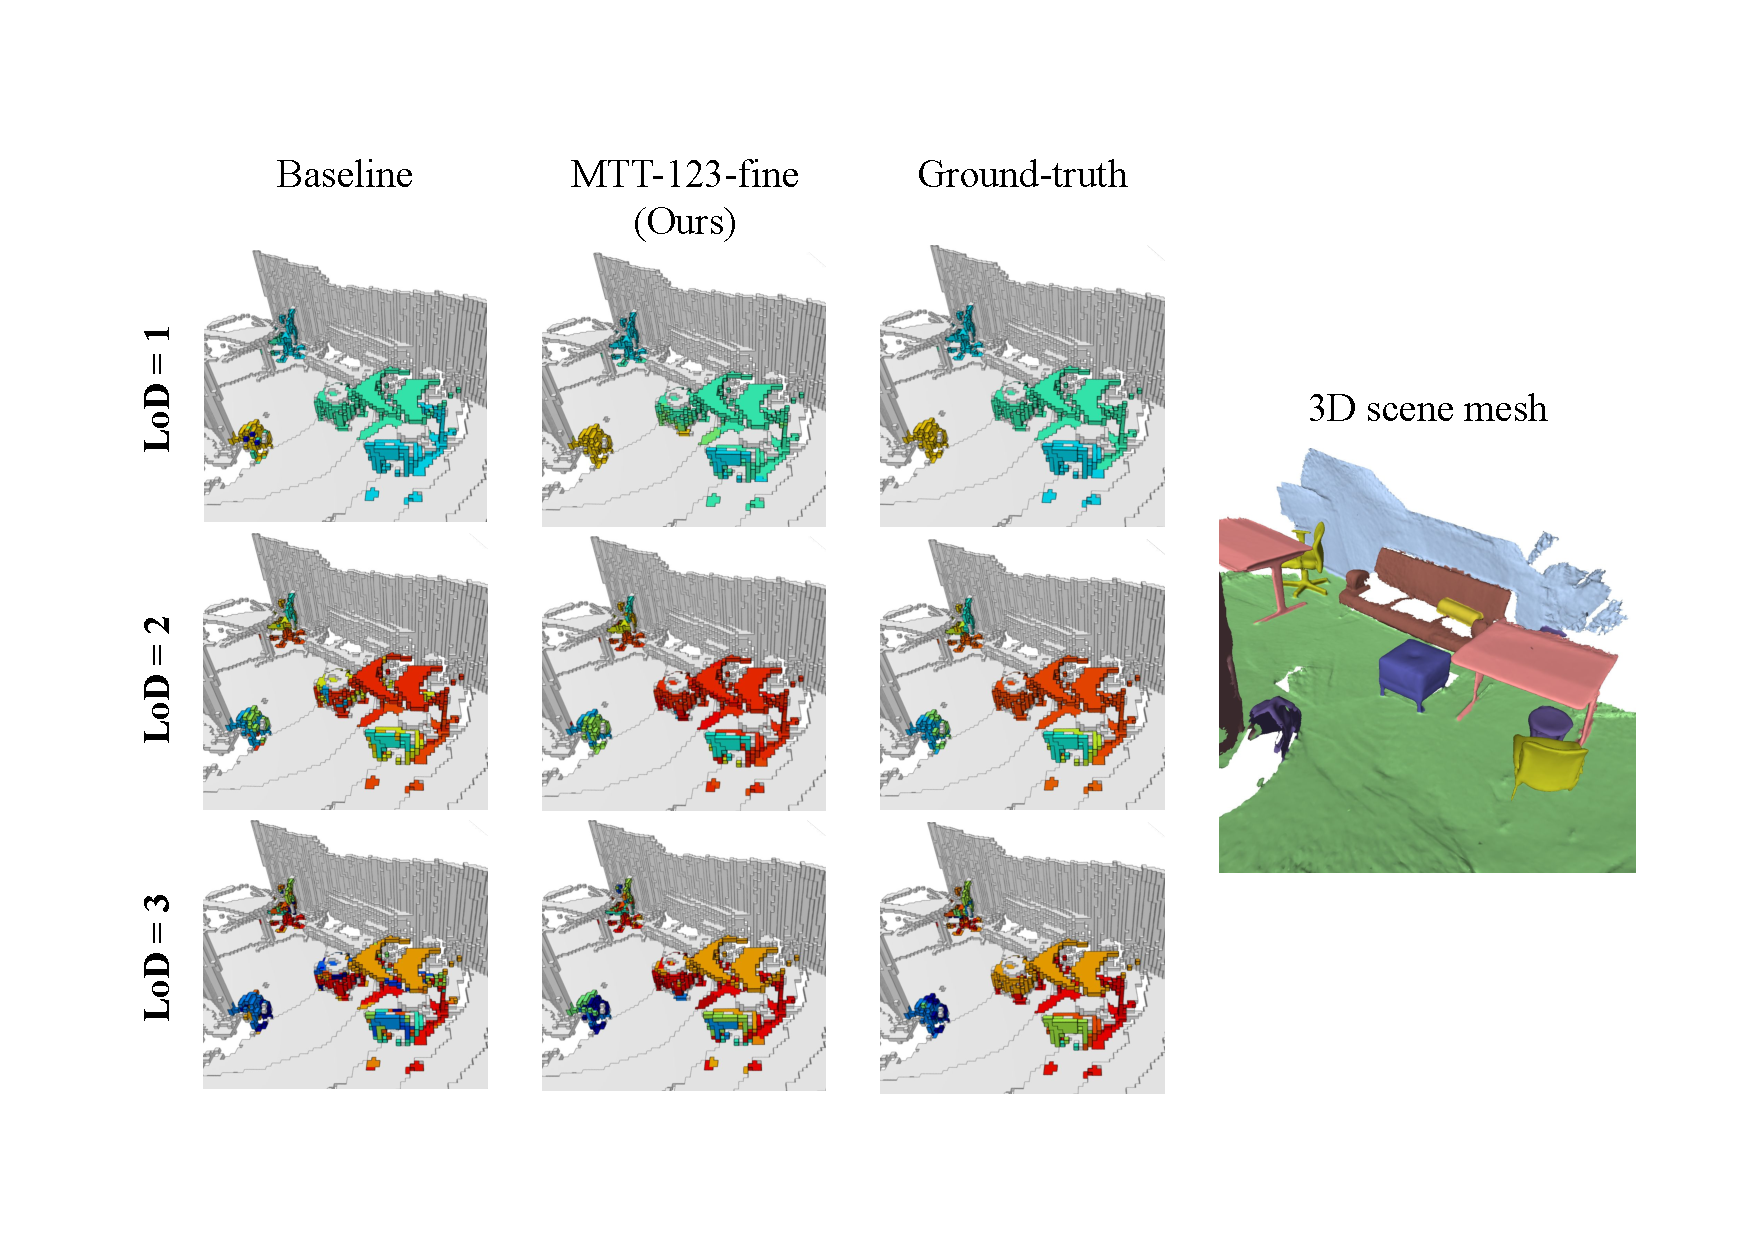
\includegraphics[width=0.99\textwidth]{Figures/scan2part/experiments_visual.pdf}
\caption{Qualitative hierarchical semantic segmentation results using the baseline models trained in each respective part-category level and our proposed method. Note the improved segmentation performance, particularly at finer levels in the parts taxonomy (lower row).}
\label{fig:hierarchical_seg_visual}
\end{figure}

\begin{table}[!h]

\caption{Part-level semantic segmentation performance in terms of mean IoU and mean balanced accuracy for different semantic granularities.}
\centering
\begin{tabular}{l rrr rrrr}
\toprule
 & \multicolumn{3}{c}{mAcc,\,\% $\uparrow$} && \multicolumn{3}{c}{mIoU,\,\% $\uparrow$} \\
\cmidrule{2-4}
\cmidrule{6-8}
Configuration   & $d_1$ & $d_2$ & $d_3$ && $d_1$ & $d_2$ & $d_3$ \\
\midrule
Base coarse     &  62.6 & ---   & ---   &&  22.5 & ---   & ---   \\
Base middle     &  \textbf{64.1} &  \textbf{57.9} & ---   &&  23.0 &  13.1 & ---   \\
Base fine       &  54.2 &  47.1 &  31.0 &&   9.5 &  \textbf{17.7} &   5.8 \\
% Base coarse (nw) & 71.74 & --- & --- & 27.15 & --- & --- \\
% Base coarse (bg) & 88.78 & --- & --- &  1.8  & --- & --- \\
\midrule
MTT-12          &  63.4 &  53.5 & ---   &&  \textbf{28.7} &  15.9 & ---   \\
MTT-123-coarse  &  63.5 &  56.2 &  32.5 &&  23.3 &  12.0 &   6.3 \\
MTT-123-fine    &  60.7 &  52.6 &  \textbf{34.7} &&  21.9 &  12.1 &   \textbf{6.7} \\
\midrule
Num. classes    &    13 &    36 &    79 &&    13 &    36 &    79 \\
\bottomrule
\end{tabular}
\label{tab:semseg}

\end{table}

\paragraph{Hierarchical semantic segmentation results. }
\label{results:hierarhical}
We present performance of hierarchical semantic segmentation in Table~\ref{tab:hierarchical_seg} and display these visually in Figure~\ref{fig:hierarchical_seg_visual}. Note that despite the baselines are focusing solely on their respective level of semantic detail, our methods is able to leverage a multi-task objective in~\eqref{eq:semseg_loss} to perform more efficient segmentation.

Hierarchical semantic segmentation is performed in a similar fashion to segmentation in MTT setting, but instead of classification of each voxel on each level of detail, heads in hierarchical model are more numerous (51 head) and perform classification of voxels to a specific sub-part class of parent class, e.g. classifying presumed chair shape to chair back, legs and seat. In this setting model is evaluated in two modes:
\begin{itemize}
    \item Oracle - in this mode mask of the parent class is taken from the ground truth data, thus each head is evaluated on it's ability to classify specific sub-parts of a certain object on specific level of detail. 
    \item Greedy - when parent object mask is predicted by heads higher in the hierarchy, predictions of the root node in hierarchy is performed first, masks for the objects are computed and heads lower on the tree evaluated only on respective mask. In this way model is evaluated as a whole top-down, which can lead to compounding of errors.
\end{itemize}
The results in Table~\ref{tab:hierarchical_seg} tell us that hierarchical model can segment specific sub-parts of many objects reasonably well. The problem arises when we try to integrate the predictions one after another in a sequential decision process, causing errors to compound and become incorrect the deeper in the tree they go.

\begin{table}[!h]

\caption{Hierarchical semantic segmentation results in terms of mean IoU and mean balanced accuracy for different semantic granularities. We include mIoU averaged over all hierarchy levels as an integral measure.}
\centering
\begin{tabular}{l rrrr r rrrr}
\toprule
  & \multicolumn{4}{c}{mAcc,\,\% $\uparrow$} 
 && \multicolumn{4}{c}{mIoU,\,\% $\uparrow$} \\
\cmidrule{2-5}
\cmidrule{7-10}
Configuration           & $d_1$ & $d_2$ & $d_3$ &  avg. && $d_1$ & $d_2$ & $d_3$ & avg. \\
\midrule
**Oracle (top-down)        &  58.5 &  82.0 &  70.9 &  70.5 &&   15.8 &  43.3 &  36.2& 31.8 \\
\midrule
Base fine (bottom-up)    &  54.2 &  47.1 &  31.0 &  44.1 &&   9.5 &  \textbf{17.7} &   5.8 & 11.0 \\
Greedy (top-down)        &  30.9 &  16.4 &   9.2 &  18.8 &&  19.0 &   9.2 &   4.8 & 11.0 \\
MTT-123-coarse           &  \textbf{63.5} &  56.2 &  32.5 &  50.7 &&  \textbf{23.3} &  12.0 &   6.3 & \textbf{13.9} \\
MTT-123-fine             &  60.7 &  52.6 &  34.7 &  49.4 &&  21.9 &  12.1 &  \textbf{6.7} & 13.6 \\
MTT-123-coarse (ensemble)&  \textbf{63.5} &	\textbf{56.8} &	33.8 & \textbf{51.4} &&   \textbf{23.3} &  11.6 &   6.1 & 13.7 \\
MTT-123-fine (ensemble)  & 60.7	 & 53.1 &	\textbf{35.6} & 49.8 &&   21.9 &  11.7 &   6.6 & 13.4 \\
\midrule
Num. classes            &    13 &    36 &    79 &       &&    13 &    36 &    79 &      \\
\bottomrule
\end{tabular}
\label{tab:hierarchical_seg}
\end{table}


\paragraph{Part instance segmentation results. }
\label{results:instance}
We present instance segmentation results in Table~\ref{table:instance}.

As expected performance of instance segmentation drops with reduction of level of detail, caused mainly by the loss of the unique properties of the instance masks, and lowering of the mean number of the voxels per instance mask.

Because we have $d_1$ level object instance mask and semantic part masks, to create $d_2, d_3$ instance masks we have a pre-processing step that selects unique semantic masks for each object instance mask separately.

\begin{table}[!h]

\caption{Instance segmentation performance in terms of mean IoU for varying levels of detail (LoD).}
\centering
\begin{tabular}{lrrr}
\toprule
Configuration       & mIoU,\,\% & AP@50,\,\%    & AR@50,\,\% \\ 
\midrule
Base coarse         & \textbf{78.6}     & \textbf{83.9} & \textbf{35.9} \\
% LoD=1, bg-push & \textbf{80.56\%} & 74.50\% & \textbf{37.11\%} \\
Base middle         & 70.5     & 54.2         & 16.6 \\
Base fine           & 64.7     & 41.4         & 15.4 \\
\bottomrule
\end{tabular}%
\label{table:instance}

\end{table}



\section{Conclusion}
We introduced a challenging benchmark for individual parts segmentation of objects in real-world, noisy indoor environments and a novel dataset Scan2Part to evaluate on. 
The core of our method is to leverage structural knowledge of objects composition to perform a variety of segmentation tasks in setting with complex geometry, high levels of uncertainty due to noise. To achieve that, we explore the part taxonomies of common objects in indoor scenes, on multiple scales and methods of compressing them for more effective use in machine learning applications. We demonstrated that specific ways of training deep segmentation models like ours Residual-U-Net style architecture are better at capturing inductive biases in structured labels on some parts of a taxonomy but not the others. Further research on relationships between structure of real-world scenes and perception models is required and we hope our benchmark and dataset will accelerate it.  


\section*{Broader Impact}
% Highlight both benefits and risks from your research. 
An obvious benefit of our research is the improved ability of automated systems to interact with complex environments which require perception on different spatial scales. It is also makes possible to extract more value from data gathered using commodity hardware like RGB-D sensors and modern smartphones. Possible risk that arises from application of technology based on our research is people relying on systems with assumption that algorithms have the same affordances as people.
% Highlight uncertainties
Composition properties of objects, parts and materials are diverse and depend on the culture, but less so with emergence of globalised manufacturing.  


% \subsubsection*{Acknowledgments}
% Use unnumbered third level headings for the acknowledgments. All
% acknowledgments, including those to funding agencies, go at the end of the paper.

% \clearpage


% \bibliographystyle{nips}
% \bibliography{references}


% \clearpage


% \appendix
% \section{Full results of Segmentation models}

\begin{table}[!htb]
\caption{Full dataset and testset statistics. As you can see it's highly unbalanced.}
\resizebox{\textwidth}{!}{%
\begin{tabular}{l|lllll}
classes & \% in testset & \# voxel & \% voxels & \# scenes & \# inst. in testset\\ \hline
Microwave & 18.75\% & 20141 & 0.38\% & 90 & 21\\
Display & 19.36\% & 149988 & 2.84\% & 350 & 142\\
Lamp & 20.14\% & 15736 & 0.30\% & 95 & 26\\
Laptop & 19.95\% & 3950 & 0.07\% & 46 & 11\\
Bag & 19.75\% & 25225 & 0.48\% & 136 & 33\\
Storage & 19.41\% & 1833826 & 34.68\% & 866 & 496\\
Bed & 20.94\% & 504774 & 9.55\% & 271 & 69\\
Table & 20.82\% & 1268401 & 23.99\% & 1104 & 539\\
Chair & 16.95\% & 1261928 & 23.87\% & 960 & 754\\
Dishwasher & 20.99\% & 12846 & 0.24\% & 24 & 6\\
TrashCan & 18.96\% & 178648 & 3.38\% & 634 & 199\\
Vase & 20.48\% & 9989 & 0.19\% & 30 & 9\\
Keyboard & 19.63\% & 1819 & 0.03\% & 24 & 9\\
% Bowl & 28.86\% & 1178 & 0.02\% & 12 \\
% Faucet & 2.44\% & 246 & 0.00\% & 4 \\
% Clock & 12.28\% & 1742 & 0.03\% & 15 \\
% Hat & 100.00\% & 101 & 0.00\% & 1 \\
% Bottle & 0.00\% & 23 & 0.00\% & 1
\end{tabular}%
\label{tab:datasetstats}
}
\end{table}

% Please add the following required packages to your document preamble:
% \usepackage{graphicx}
{\lat
\begin{table}[!htb]
\caption{mIoU of different models for each class}
\resizebox{\textwidth}{!}{%
\begin{tabular}{l|llllll}
Classes & Original & bg & no-w & LoD=1-2 & LoD=1-3, Dec & LoD=1-3, Inc \\
\hline
Microwave & 2.05\% & 0.52\% & 3.41\% & \textbf{15.86\%} & 4.74\% & 7.99\% \\
Display & 42.28\% & 1.69\% & 41.44\% & \textbf{44.10\%} & 39.94\% & 39.01\% \\
Lamp & 17.10\% & 0.64\% & \textbf{21.85\%} & 17.81\% & 16.47\% & 9.62\% \\
Laptop & 9.80\% & 1.07\% & 5.60\% & 11.64\% & \textbf{11.91\%} & 6.91\% \\
Bag & 9.97\% & 0.78\% & 4.23\% & \textbf{11.42\%} & 7.39\% & 5.98\% \\
Storage & 47.18\% & 2.91\% & \textbf{63.40\%} & 47.10\% & 55.97\% & 44.29\% \\
Bed & 31.98\% & 5.60\% & \textbf{53.70\%} & 46.27\% & 32.73\% & 32.78\% \\
Table & 49.21\% & 3.96\% & \textbf{53.52\%} & 50.73\% & 46.14\% & 47.74\% \\
Chair & 55.13\% & 3.73\% & 65.86\% & \textbf{69.67\%} & 54.07\% & 62.05\% \\
Dishwasher & 0.00\% & 0.00\% & \textbf{8.68\%} & 0.10\% & 0.28\% & 0.00\% \\
TrashCan & 21.35\% & 1.94\% & 28.98\% & \textbf{40.64\%} & 18.46\% & 25.80\% \\
Vase & 1.83\% & 0.03\% & 2.00\% & \textbf{9.84\%} & 2.72\% & 1.00\% \\
Keyboard & 4.06\% & 0.53\% & 0.26\% & 8.15\% & \textbf{11.74\%} & 1.27\% \\
\hline
mIoU & 22.46\% & 1.80\% & 27.15\% & \textbf{28.72\%} & 23.27\% & 21.88\%
\end{tabular}%
\label{tab:lodmiou1table}
}
\end{table}}

{\lat
\begin{table}[!htb]
\caption{results of the models on Instance Segmentation task, original model and with background push}
\resizebox{\textwidth}{!} & \textbf{87.50\%} & \textbf{33.33\%} & 80.59\% & 75.00\% & 28.57\% \\
Display & \textbf{76.15\%} & \textbf{64.62\%} & 29.58\% & 73.59\% & 64.00\% & \textbf{33.80\%} \\
Lamp & 65.29\% & 75.00\% & \textbf{34.62\%} & \textbf{70.64\%} & \textbf{77.78\%} & 26.92\% \\
Laptop & \textbf{50.44\%} & \textbf{100.00\%} & \textbf{9.09\%} & NaN & 0.00\% & 0.00\% \\
Bag & 89.19\% & \textbf{100.00\%} & \textbf{33.33\%} & \textbf{91.70\%} & 75.00\% & 27.27\% \\
Storage & \textbf{82.01\%} & 71.71\% & 37.30\% & 81.44\% & \textbf{74.70\%} & \textbf{38.10\%} \\
Bed & \textbf{79.55\%} & 62.86\% & 63.77\% & 78.38\% & \textbf{74.29\%} & \textbf{75.36\%} \\
Table & 77.34\% & 77.10\% & 42.49\% & \textbf{80.35\%} & \textbf{81.37\%} & \textbf{46.20\%} \\
Chair & 82.88\% & 82.14\% & 30.50\% & \textbf{86.01\%} & \textbf{86.79\%} & \textbf{32.23\%} \\
Dishwasher & 71.32\% & 100.00\% & 66.67\% & \textbf{72.66\%} & \textbf{100.00\%} & \textbf{66.67\%} \\
TrashCan & 87.22\% & \textbf{86.18\%} & \textbf{53.27\%} & \textbf{89.88\%} & 85.12\% & 51.76\% \\
Vase & \textbf{90.83\%} & 100.00\% & 33.33\% & 80.89\% & \textbf{100.00\%} & \textbf{55.56\%} \\
\hline
mIoU / mAP & 78.60\% & \textbf{83.93\%} & 35.94\% & \textbf{80.56\%} & 74.50\% & \textbf{37.11\%}
\end{tabular}%
\label{tab:lod1instsegresults}
}
\end{table}}


\begin{figure}[!htb]
\centering
\label{fig:partnet_to_scannet_labeling}
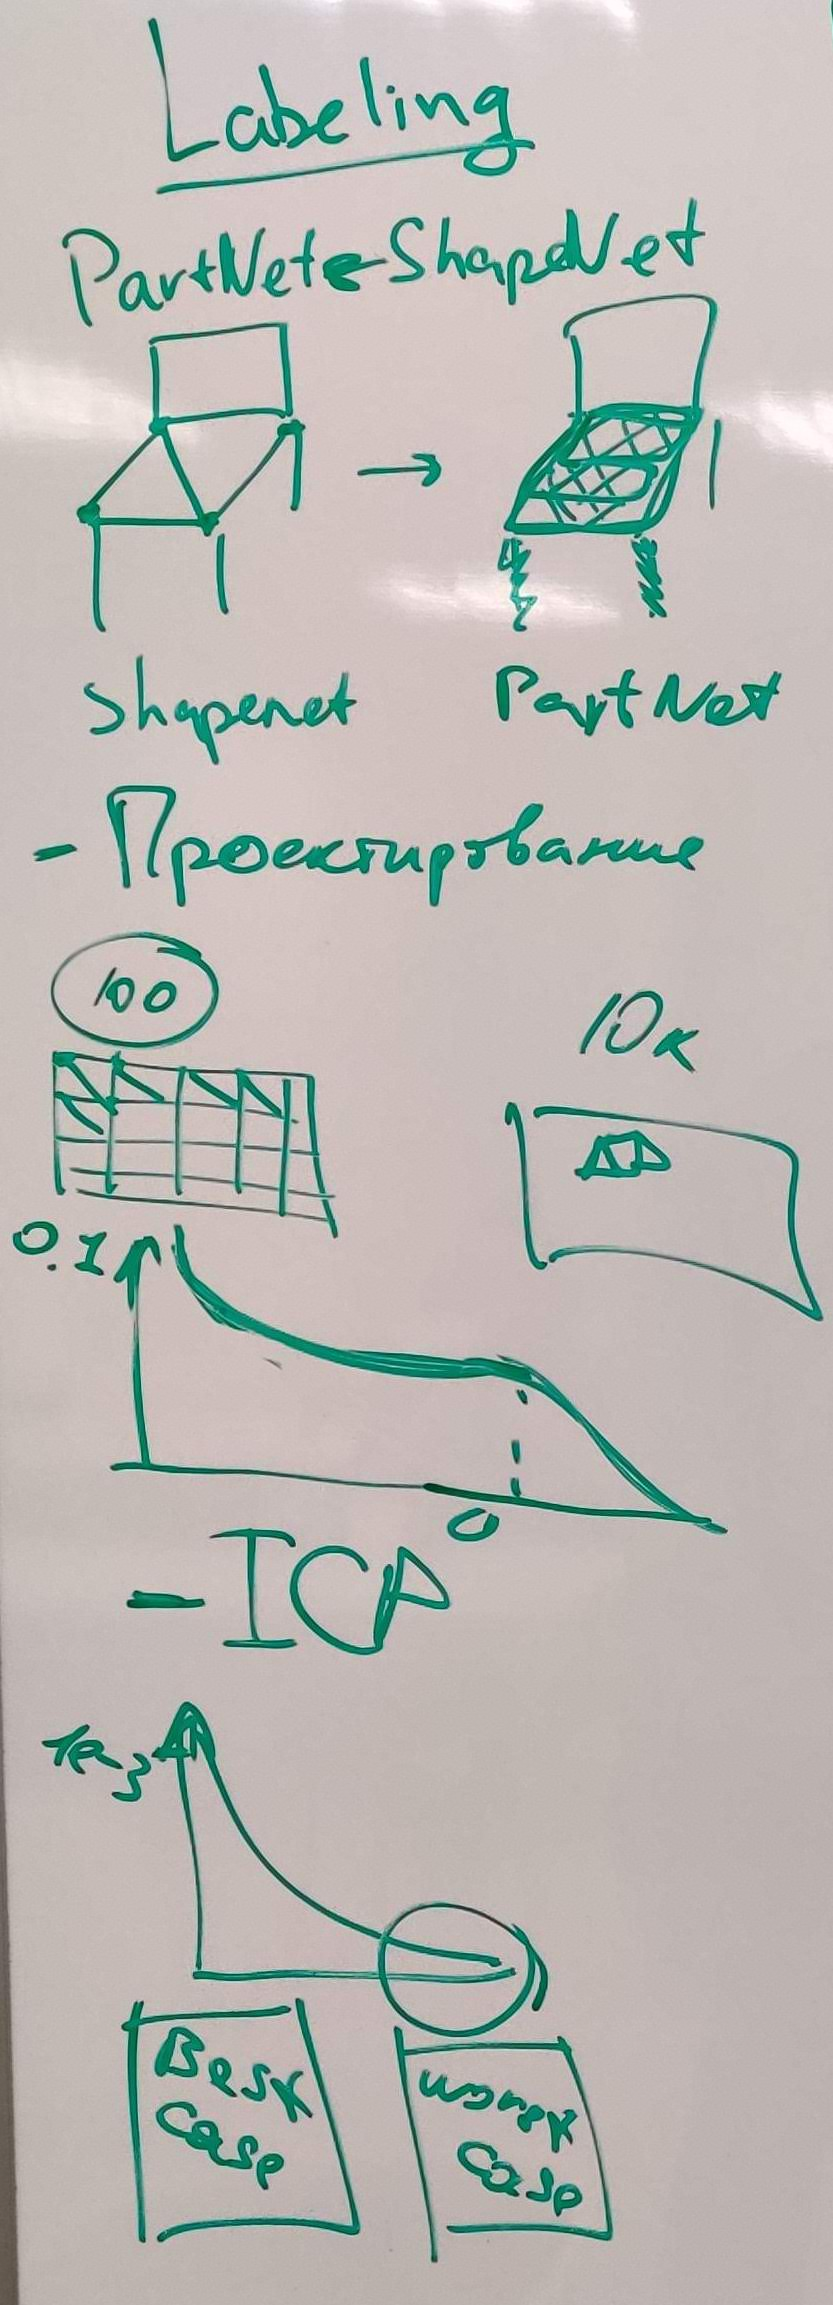
\includegraphics[trim=0 0 0 0, max width=0.25\textwidth]{images/partnet_to_scannet_labeling.jpg}
\caption{partnet to scannet labeling (a,b,c)}
% \end{wrapfigure}
\end{figure}

\begin{figure}[!htb]
\label{fig:scannet_overview}
  \centering
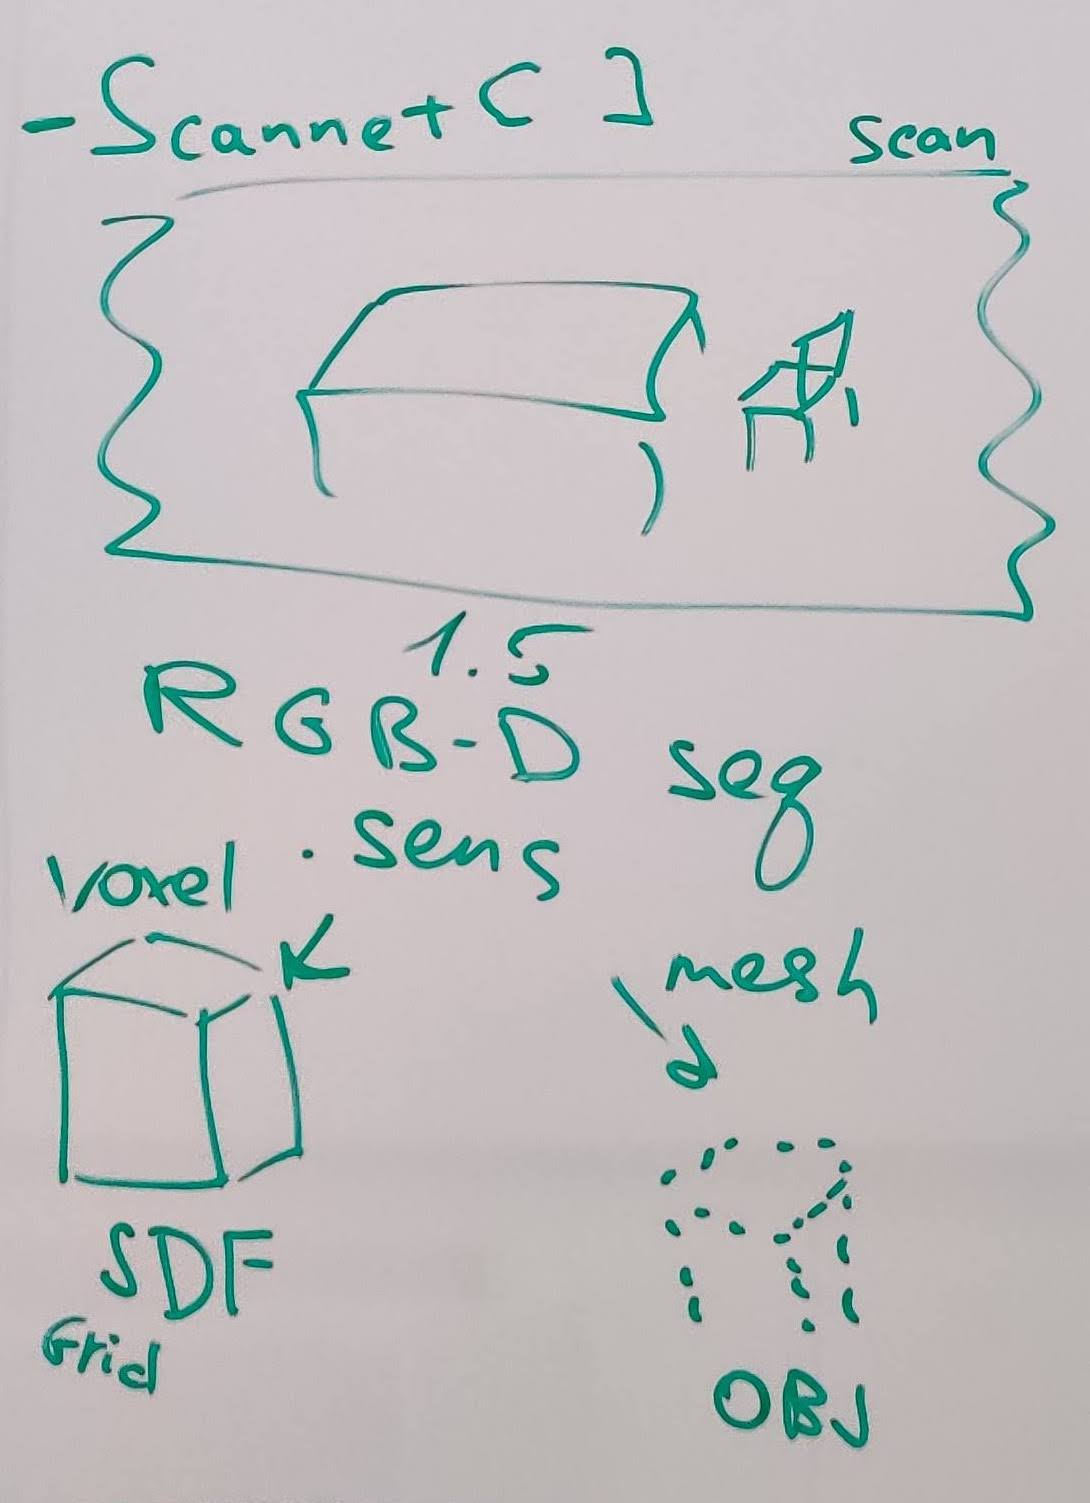
\includegraphics[trim=0 0 0 0, max width=0.5\textwidth]{images/scannet_overview.jpg}
\caption{scannet overview}
\end{figure}

\begin{figure}[!htb]
\label{fig:Scan2Cad_overview}
\centering
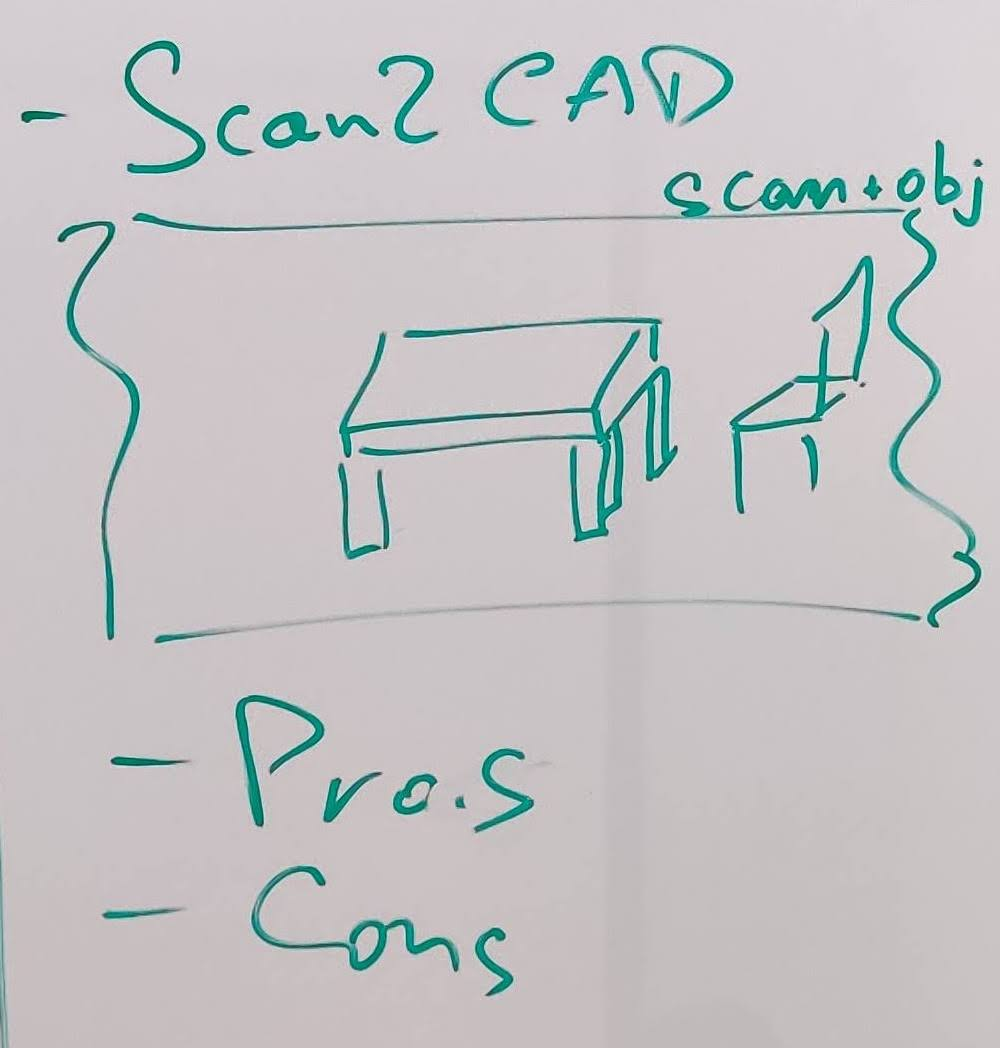
\includegraphics[trim=0 0 0 0, max width=0.5\textwidth]{images/Scan2Cad_overview.jpg}
\caption{Scan2Cad overview}
\end{figure}



\begin{table}[]
\caption{Proportions of ShapeNet semantic classes present in Scan2Cad dataset}
\label{table:scan2part_proportions}
\begin{tabular}{l|l|l}
Class ID & overlap? & class name \\
\hline
04379243 & 99.0\% (822/830) & table \\ \hline
02747177 & 98.9\% (88/89) & ashcan,trash can,garbage can,wastebin,ash bin,ash-bin \\ \hline
03211117 & 97.6\% (161/165) & display,video display \\ \hline
03761084 & 97.3\% (36/37) & microwave,microwave oven \\ \hline
03337140 & 97.1\% (68/70) & file,file cabinet,filing cabinet \\ \hline
03001627 & 96.9\% (632/652) & chair \\ \hline
02871439 & 96.7\% (145/150) & bookshelf \\ \hline
02933112 & 94.8\% (294/310) & cabinet \\ \hline
02818832 & 94.0\% (47/50) & bed \\ \hline
03991062 & 91.7\% (11/12) & pot,flowerpot \\ \hline
03207941 & 85.7\% (12/14) & dishwasher,dish washer,dishwashing machine \\ \hline
03085013 & 81.8\% (9/11) & computer keyboard,keypad \\ \hline
03325088 & 57.1\% (4/7) & faucet,spigot \\ \hline
02876657 & 50.0\% (1/2) & bottle \\ \hline
02808440 & 26.0\% (25/96) & bathtub,bathing tub,bath,tub \\ \hline
02801938 & 9.4\% (3/32) & basket,handbasket \\ \hline
04256520 & 8.1\% (20/247) & sofa,couch,lounge \\ \hline
02946921 & 0.0\% (0/1) & can,tin,tin can \\ \hline
03938244 & 0.0\% (0/5) & pillow \\ \hline
02828884 & 0.0\% (0/28) & bench \\ \hline
04554684 & 0.0\% (0/37) & washer,automatic washer,washing machine \\ \hline
03928116 & 0.0\% (0/25) & piano,pianoforte,forte-piano \\ \hline
03790512 & 0.0\% (0/4) & motorcycle,bike \\ \hline
03691459 & 0.0\% (0/2) & loudspeaker,speaker,speaker unit,loudspeaker system \\ \hline
03467517 & 0.0\% (0/6) & guitar \\ \hline
04330267 & 0.0\% (0/36) & stove \\ \hline
04401088 & 0.0\% (0/1) & telephone,phone,telephone set \\ \hline
04004475 & 0.0\% (0/31) & printer,printing machine \\ \hline
Total:    & 81.2\% (2477/3049) &         \\
\end{tabular}
\end{table}




\subsection{Scene labeling}

\textbf{PartNet -> Shapenet.} The PartNet \cite{mo2019partnet} is a hierarchical instance-level parts dataset of labels for the subset of the ShapeNet database. The PartNet dataset is the only dataset that has a deep hierarchical structure compared to other part annotation datasets, e.g.,  \cite{Yi16}. However, the PartNet dataset does not preserve the original ShapeNet coordinate system in the sense that each object is rotated in an unspecified order. For mapping labels to Scannet scenes, we need to restore the original coordinate system. To find the rotation matrix between coordinate systems, we use the following alignment process for each object: \begin{enumerate}
    \item we sample 20 different rotation angles corresponding to the vertices of the convex regular dodecahedron;
    \item each rotation angle is represented as the initial alignment matrix of the object for alignment;
    \item we perform Point-to-point ICP alignment separately for each initial alignment matrix;
    \item we select the best one out of 20 alignment results where the distance between the original ShapeNet shape and the rotated PartNet shape is minimal.
\end{enumerate}

\textbf{Shapenet -> Scannet (Scan2CAD).} The Scan2CAD \cite{avetisyan2019scan2cad} is a dataset that aligns CAD objects from ShapeNet \cite{chang2015shapenet} database to scenes from Scannet. Using the marching cubes algorithm, we obtained  voxelized versions of scenes from ScanNet dataset with object type labels and mapping of coordinate systems from ScanNet to ShapeNet.  Finally, we  calculate the position of CAD object parts in the scene coordinate system and calculate relative volume in specific voxels thus projecting part labels on the scene. \DZ{unclear what relative volume is needed for here}

Under closer examination, we discovered that most of the parts do not have a unique shape making the task of instance segmentation for parts very hard to solve and not necessary for practical scene segmentation task. \DZ{unclear}



% \end{document}
\newpage 

\section{Conclusion}
\label{sect:conclusion}

% Discuss your conclusions in order of most to least important.

In this chapter, we have compared the image-based domain adaptation techniques for face recognition in the presence of strong image degradation. We consider the recently proposed CycleGAN approach for learning mappings between the two domains of surveillance data and Internet face images. We demonstrate that the strategy of transferring the labeled Internet data to the surveillance domain and subsequent retraining the face recognition network helps to improve the recognition quality on real surveillance test data. We have investigated the variants of this approach, and have demonstrated that training on both transferred and original Internet data leads to the optimal performance. Finally, we show that in the case of our domain pair, the image-level adaptation approach outperforms feature-level domain adaptation. 

%Compare your results with those from other studies: Are they consistent? If not, discuss possible reasons for the difference.
We found our results consistent with \cite{SohnLZY0C17}, where face recognition for the low-quality is also considered. In \cite{SohnLZY0C17},  verification accuracy was improved using carefully chosen data augmentation. It is an interesting fact, that the improvement remained noticeable even when the data augmentation and the feature-level domain adaptation were applied simultaneously. Here, in contrast, we suggest performing the data augmentation in a more automatic way. Although we do not experiment with the combination of feature-level and image-level approaches to domain adaptation, we compare them independently. The combination of these adaptation techniques may further improve the results.


% Mention any inconclusive results and explain them as best you can. You may suggest additional experiments needed to clarify your results.
In our experiments, best results were achieved with training on both domains. An explanation can be given that the domain transfer model is imperfect and may push different images of the same identity too far as we do not use any kind of verification loss for training (ideally, this would require another pre-trained network for the low-quality domain, which essentially is the goal of this work). Therefore, keeping the initial data in the training set may result in less overfitting. %This can be explained by the fact that our target domain is not uniform in terms of data quality. We use two parts of the same track to generate matching pairs for each identity: e.g. these parts of each track differ in resolution (see \ref{fig:lr_hr_gan_res_ytube_initial_degraded}, columns $1$ and $3$). Therefore, using training data of diverse quality may lead to better results.  -- not true, checked.

% Briefly describe the limitations of your study to show reviewers and readers that you have considered your experiment’s weaknesses. Many researchers are hesitant to do this as they feel it highlights the weaknesses in their research to the editor and reviewer. However doing this actually makes a positive impression of your paper as it makes it clear that you have an in depth understanding of your topic and can think objectively of your research.

As an important negative result, we show that using CycleGAN-based restoration of lower-quality domain images by transferring them to the higher-quality domain does not bring consistent improvement to the recognition performance. We speculate that such transfer may distort some details of the images in a non-identity preserving way.

Our study considers a practically important domain of image data. 
We note, however, that our findings might not transfer to other pairs of domains in image adaptation.


% Discuss what your results may mean for researchers in the same field as you, researchers in other fields, and the general public. How could your findings be applied?
 
% State how your results extend the findings of previous studies.
% If your findings are preliminary, suggest future studies that need to be carried out.
% At the end of your Discussion and Conclusions sections, state your main conclusions once again.



%% ----------------------------------------------------------------
% Now begin the Appendices, including them as separate files

\addtocontents{toc}{\vspace{2em}} % Add a gap in the Contents, for aesthetics

\appendix 

%\mbox{}
 



% Cue to tell LaTeX that the following 'chapters' are Appendices

%\chapter{An Appendix}

Lorem ipsum dolor sit amet, consectetur adipiscing elit. Vivamus at pulvinar nisi. Phasellus hendrerit, diam placerat interdum iaculis, mauris justo cursus risus, in viverra purus eros at ligula. Ut metus justo, consequat a tristique posuere, laoreet nec nibh. Etiam et scelerisque mauris. Phasellus vel massa magna. Ut non neque id tortor pharetra bibendum vitae sit amet nisi. Duis nec quam quam, sed euismod justo. Pellentesque eu tellus vitae ante tempus malesuada. Nunc accumsan, quam in congue consequat, lectus lectus dapibus erat, id aliquet urna neque at massa. Nulla facilisi. Morbi ullamcorper eleifend posuere. Donec libero leo, faucibus nec bibendum at, mattis et urna. Proin consectetur, nunc ut imperdiet lobortis, magna neque tincidunt lectus, id iaculis nisi justo id nibh. Pellentesque vel sem in erat vulputate faucibus molestie ut lorem.

Quisque tristique urna in lorem laoreet at laoreet quam congue. Donec dolor turpis, blandit non imperdiet aliquet, blandit et felis. In lorem nisi, pretium sit amet vestibulum sed, tempus et sem. Proin non ante turpis. Nulla imperdiet fringilla convallis. Vivamus vel bibendum nisl. Pellentesque justo lectus, molestie vel luctus sed, lobortis in libero. Nulla facilisi. Aliquam erat volutpat. Suspendisse vitae nunc nunc. Sed aliquet est suscipit sapien rhoncus non adipiscing nibh consequat. Aliquam metus urna, faucibus eu vulputate non, luctus eu justo.

Donec urna leo, vulputate vitae porta eu, vehicula blandit libero. Phasellus eget massa et leo condimentum mollis. Nullam molestie, justo at pellentesque vulputate, sapien velit ornare diam, nec gravida lacus augue non diam. Integer mattis lacus id libero ultrices sit amet mollis neque molestie. Integer ut leo eget mi volutpat congue. Vivamus sodales, turpis id venenatis placerat, tellus purus adipiscing magna, eu aliquam nibh dolor id nibh. Pellentesque habitant morbi tristique senectus et netus et malesuada fames ac turpis egestas. Sed cursus convallis quam nec vehicula. Sed vulputate neque eget odio fringilla ac sodales urna feugiat.

Phasellus nisi quam, volutpat non ullamcorper eget, congue fringilla leo. Cras et erat et nibh placerat commodo id ornare est. Nulla facilisi. Aenean pulvinar scelerisque eros eget interdum. Nunc pulvinar magna ut felis varius in hendrerit dolor accumsan. Nunc pellentesque magna quis magna bibendum non laoreet erat tincidunt. Nulla facilisi.

Duis eget massa sem, gravida interdum ipsum. Nulla nunc nisl, hendrerit sit amet commodo vel, varius id tellus. Lorem ipsum dolor sit amet, consectetur adipiscing elit. Nunc ac dolor est. Suspendisse ultrices tincidunt metus eget accumsan. Nullam facilisis, justo vitae convallis sollicitudin, eros augue malesuada metus, nec sagittis diam nibh ut sapien. Duis blandit lectus vitae lorem aliquam nec euismod nisi volutpat. Vestibulum ornare dictum tortor, at faucibus justo tempor non. Nulla facilisi. Cras non massa nunc, eget euismod purus. Nunc metus ipsum, euismod a consectetur vel, hendrerit nec nunc.	% Appendix Title

%\input{Appendices/AppendixB} % Appendix Title

%\input{Appendices/AppendixC} % Appendix Title

\addtocontents{toc}{\vspace{2em}}  % Add a gap in the Contents, for aesthetics
\backmatter

%% ----------------------------------------------------------------
\label{Bibliography}
\lhead{\emph{Bibliography}}  % Change the left side page header to "Bibliography"
\bibliographystyle{plainnat}  % Use the "unsrtnat" BibTeX style for formatting the Bibliography
\bibliography{Bibliography.bib}  % The references (bibliography) information are stored in the file named "Bibliography.bib"


\begin{titlepage}
 \begin{center}
 \phantom{a}\vspace{13.2cm}
 

\includegraphics[width=6cm]{sk.png}
  
 
  \vspace{7cm}
  
  2020

  \vspace{2cm}

  
  
  
 \end{center}

\end{titlepage}
\end{document}  % The End
%% ---------------------------------------------------------------- 
